\documentclass[12pt,english,a4paper,titlepage,cleardoublepage=empty,dottedtoc]{report}



% % % additions by tompollard START -->

% Overwrite \begin{figure}[htbp] with \begin{figure}[H]
% TODO: delete if images position is awkward
\usepackage{float}
\let\origfigure=\figure
\let\endorigfigure=\endfigure
\renewenvironment{figure}[1][]{%
\origfigure[b]
}{%
\endorigfigure
}

% TP: hack to truncate list of figures/tables.
\usepackage{truncate}
\usepackage{caption}
\usepackage{tocloft}
% TP: end hack

% % % <-- END additions by tompollard



\usepackage{lmodern}
\usepackage{setspace}
\setstretch{1.2}
\usepackage{amssymb,amsmath}
\usepackage{ifxetex,ifluatex}
\usepackage{fixltx2e} % provides \textsubscript
\ifnum 0\ifxetex 1\fi\ifluatex 1\fi=0 % if pdftex
  \usepackage[T1]{fontenc}
  \usepackage[utf8]{inputenc}
\else % if luatex or xelatex
  \ifxetex
    \usepackage{mathspec}
  \else
    \usepackage{fontspec}
  \fi
  \defaultfontfeatures{Ligatures=TeX,Scale=MatchLowercase}
\fi
% use upquote if available, for straight quotes in verbatim environments
\IfFileExists{upquote.sty}{\usepackage{upquote}}{}
% use microtype if available
\IfFileExists{microtype.sty}{%
\usepackage{microtype}
\UseMicrotypeSet[protrusion]{basicmath} % disable protrusion for tt fonts
}{}
\usepackage[unicode=true]{hyperref}
\hypersetup{
            pdftitle={Open Specification of a user-controlled Web Service for Personal Data},
            pdfauthor={G. Jahn},
            pdfkeywords={personal data store; personal data as a service; web service architecture; open specification; masters thesis},
            pdfborder={0 0 0},
            breaklinks=true}
\urlstyle{same}  % don't use monospace font for urls
\ifnum 0\ifxetex 1\fi\ifluatex 1\fi=0 % if pdftex
  \usepackage[shorthands=off,main=english]{babel}
\else
  \usepackage{polyglossia}
  \setmainlanguage[]{english}
\fi

% added 20170205 -->
% NOTE: Replace "english" in "captionsenglish" with the language you use
\addto\captionsenglish{
  \renewcommand{\contentsname}
    {Table of Contents}
}
% added 20170205 <--

\usepackage{color}
\usepackage{fancyvrb}
\newcommand{\VerbBar}{|}
\newcommand{\VERB}{\Verb[commandchars=\\\{\}]}
\DefineVerbatimEnvironment{Highlighting}{Verbatim}{commandchars=\\\{\}}
% Add ',fontsize=\small' for more characters per line
\usepackage{framed}
\definecolor{shadecolor}{RGB}{248,248,248}
\newenvironment{Shaded}{\begin{snugshade}}{\end{snugshade}}
\newcommand{\KeywordTok}[1]{\textcolor[rgb]{0.13,0.29,0.53}{\textbf{{#1}}}}
\newcommand{\DataTypeTok}[1]{\textcolor[rgb]{0.13,0.29,0.53}{{#1}}}
\newcommand{\DecValTok}[1]{\textcolor[rgb]{0.00,0.00,0.81}{{#1}}}
\newcommand{\BaseNTok}[1]{\textcolor[rgb]{0.00,0.00,0.81}{{#1}}}
\newcommand{\FloatTok}[1]{\textcolor[rgb]{0.00,0.00,0.81}{{#1}}}
\newcommand{\ConstantTok}[1]{\textcolor[rgb]{0.00,0.00,0.00}{{#1}}}
\newcommand{\CharTok}[1]{\textcolor[rgb]{0.31,0.60,0.02}{{#1}}}
\newcommand{\SpecialCharTok}[1]{\textcolor[rgb]{0.00,0.00,0.00}{{#1}}}
\newcommand{\StringTok}[1]{\textcolor[rgb]{0.31,0.60,0.02}{{#1}}}
\newcommand{\VerbatimStringTok}[1]{\textcolor[rgb]{0.31,0.60,0.02}{{#1}}}
\newcommand{\SpecialStringTok}[1]{\textcolor[rgb]{0.31,0.60,0.02}{{#1}}}
\newcommand{\ImportTok}[1]{{#1}}
\newcommand{\CommentTok}[1]{\textcolor[rgb]{0.56,0.35,0.01}{\textit{{#1}}}}
\newcommand{\DocumentationTok}[1]{\textcolor[rgb]{0.56,0.35,0.01}{\textbf{\textit{{#1}}}}}
\newcommand{\AnnotationTok}[1]{\textcolor[rgb]{0.56,0.35,0.01}{\textbf{\textit{{#1}}}}}
\newcommand{\CommentVarTok}[1]{\textcolor[rgb]{0.56,0.35,0.01}{\textbf{\textit{{#1}}}}}
\newcommand{\OtherTok}[1]{\textcolor[rgb]{0.56,0.35,0.01}{{#1}}}
\newcommand{\FunctionTok}[1]{\textcolor[rgb]{0.00,0.00,0.00}{{#1}}}
\newcommand{\VariableTok}[1]{\textcolor[rgb]{0.00,0.00,0.00}{{#1}}}
\newcommand{\ControlFlowTok}[1]{\textcolor[rgb]{0.13,0.29,0.53}{\textbf{{#1}}}}
\newcommand{\OperatorTok}[1]{\textcolor[rgb]{0.81,0.36,0.00}{\textbf{{#1}}}}
\newcommand{\BuiltInTok}[1]{{#1}}
\newcommand{\ExtensionTok}[1]{{#1}}
\newcommand{\PreprocessorTok}[1]{\textcolor[rgb]{0.56,0.35,0.01}{\textit{{#1}}}}
\newcommand{\AttributeTok}[1]{\textcolor[rgb]{0.77,0.63,0.00}{{#1}}}
\newcommand{\RegionMarkerTok}[1]{{#1}}
\newcommand{\InformationTok}[1]{\textcolor[rgb]{0.56,0.35,0.01}{\textbf{\textit{{#1}}}}}
\newcommand{\WarningTok}[1]{\textcolor[rgb]{0.56,0.35,0.01}{\textbf{\textit{{#1}}}}}
\newcommand{\AlertTok}[1]{\textcolor[rgb]{0.94,0.16,0.16}{{#1}}}
\newcommand{\ErrorTok}[1]{\textcolor[rgb]{0.64,0.00,0.00}{\textbf{{#1}}}}
\newcommand{\NormalTok}[1]{{#1}}
\usepackage{longtable,booktabs}
% Fix footnotes in tables (requires footnote package)
\IfFileExists{footnote.sty}{\usepackage{footnote}\makesavenoteenv{long table}}{}
\usepackage{graphicx,grffile}
\makeatletter
\def\maxwidth{\ifdim\Gin@nat@width>\linewidth\linewidth\else\Gin@nat@width\fi}
\def\maxheight{\ifdim\Gin@nat@height>\textheight\textheight\else\Gin@nat@height\fi}
\makeatother
% Scale images if necessary, so that they will not overflow the page
% margins by default, and it is still possible to overwrite the defaults
% using explicit options in \includegraphics[width, height, ...]{}
\setkeys{Gin}{width=\maxwidth,height=\maxheight,keepaspectratio}
% Make links footnotes instead of hotlinks:
\renewcommand{\href}[2]{#2\footnote{\url{#1}}}
\IfFileExists{parskip.sty}{%
\usepackage{parskip}
}{% else
\setlength{\parindent}{0pt}
\setlength{\parskip}{6pt plus 2pt minus 1pt}
}
\setlength{\emergencystretch}{3em}  % prevent overfull lines
\providecommand{\tightlist}{%
  \setlength{\itemsep}{0pt}\setlength{\parskip}{0pt}}
\setcounter{secnumdepth}{2}

% set default figure placement to htbp
\makeatletter
\def\fps@figure{htbp}
\makeatother


% Headers and page numbering
\usepackage{fancyhdr}
% 20170205 changed from \pagestyle{plain}
\pagestyle{fancy}
% added 20170205 -->
\fancyhf{}
\renewcommand{\headrulewidth}{0pt}
\fancyhead[OL]{\leftmark}
\fancyfoot[C]{\thepage}
% added 20170205 <--

% Table package
\usepackage{ctable}% http://ctan.org/pkg/ctable

% Deal with 'LaTeX Error: Too many unprocessed floats.'
\usepackage{morefloats}
% or use \extrafloats{100}
% add some \clearpage

% % Chapter header
% \usepackage{titlesec, blindtext, color}
% \definecolor{gray75}{gray}{0.75}
% \newcommand{\hsp}{\hspace{20pt}}
% \titleformat{\chapter}[hang]{\Huge\bfseries}{\thechapter\hsp\textcolor{gray75}{|}\hsp}{0pt}{\Huge\bfseries}

% % Fonts and typesetting
% \setmainfont[Scale=1.1]{Helvetica}
% \setsansfont[Scale=1.1]{Verdana}

% FONTS
\usepackage{xunicode}
\usepackage{xltxtra}
\defaultfontfeatures{Mapping=tex-text} % converts LaTeX specials (``quotes'' --- dashes etc.) to unicode
% \setromanfont[Scale=1.01,Ligatures={Common},Numbers={OldStyle}]{Palatino}
% \setromanfont[Scale=1.01,Ligatures={Common},Numbers={OldStyle}]{Adobe Caslon Pro}
%Following line controls size of code chunks
% \setmonofont[Scale=0.9]{Monaco}
%Following line controls size of figure legends
% \setsansfont[Scale=1.2]{Optima Regular}

%Attempt to set math size
%First size must match the text size in the document or command will not work
%\DeclareMathSizes{display size}{text size}{script size}{scriptscript size}.
\DeclareMathSizes{12}{13}{7}{7}

% ---- CUSTOM AMPERSAND
% \newcommand{\amper}{{\fontspec[Scale=.95]{Adobe Caslon Pro}\selectfont\itshape\&}}

% HEADINGS
\usepackage{sectsty}
\usepackage[normalem]{ulem}
\sectionfont{\rmfamily\mdseries\Large}
\subsectionfont{\rmfamily\mdseries\scshape\large}
\subsubsectionfont{\rmfamily\bfseries\upshape\large}
% \sectionfont{\rmfamily\mdseries\Large}
% \subsectionfont{\rmfamily\mdseries\scshape\normalsize}
% \subsubsectionfont{\rmfamily\bfseries\upshape\normalsize}

% Set figure legends and captions to be smaller sized sans serif font
\usepackage[font={footnotesize,sf}]{caption}

\usepackage{siunitx}

% Adjust spacing between lines to 1.5
\usepackage{setspace}
% \onehalfspacing
%\doublespacing
\raggedbottom

% Set margins
\usepackage[top=1.5in,bottom=1.5in,left=1.5in,right=1.4in]{geometry}
% \setlength\parindent{0.4in} % indent at start of paragraphs (set to 0.3?)
\setlength{\parskip}{9pt}

% Add space between pararaphs
% http://texblog.org/2012/11/07/correctly-typesetting-paragraphs-in-latex/
% \usepackage{parskip}
% \setlength{\parskip}{\baselineskip}

% Set colour of links to black so that they don't show up when printed
\usepackage{hyperref}
\hypersetup{colorlinks=false, linkcolor=black}

% added 20170130 -->
% to fix URLs not willing to break in bibs
% src https://tex.stackexchange.com/questions/3033/forcing-linebreaks-in-url
\usepackage{url}
\def\UrlOrds{\do\*\do\-\do\~\do\'\do\"\do\-}%
\makeatletter
\g@addto@macro{\UrlBreaks}{\UrlOrds}
\makeatother
% added 20170130 <--

% Tables
\usepackage{booktabs}
\usepackage{threeparttable}
\usepackage{array}
\newcolumntype{x}[1]{%
>{\centering\arraybackslash}m{#1}}%

% Allow for long captions and float captions on opposite page of figures
% \usepackage[rightFloats, CaptionBefore]{fltpage}

% Don't let floats cross subsections
% \usepackage[section,subsection]{extraplaceins}


% Chapter styling
% src: https://github.com/chiakaivalya/thesis-markdown-pandoc/blob/master/preamble.tex#L26
\usepackage[grey]{quotchap}
\makeatletter
\renewcommand*{\chapnumfont}{%
  \usefont{T1}{\@defaultcnfont}{b}{n}\fontsize{80}{100}\selectfont% Default: 100/130
  \color{chaptergrey}%
}
\makeatother


% added 20170205 -->
% make block quote latin again
\let\origquote\quote
\let\endorigquote\endquote
\renewenvironment{quote}{%
    \origquote
    \itshape
}
{\endorigquote}
% added 20170205 <--

\title{Open Specification of a user-controlled Web Service for Personal Data}
\providecommand{\subtitle}[1]{}
\subtitle{Master Thesis}
\author{G. Jahn}
\date{\today}

\begin{document}
\maketitle
\begin{abstract}
Often data is referred to as \emph{the oil of the 21st century}. Whereas
recovering petroleum or coal is governed b certain rules and
legislation, at the same time however vast amounts of personal data is
harvested from all sorts of resources with no working restrictions or
asking for permission. Well air-conditioned data centers are mining to
the clock of dozens of CPUs. Eager to discover even the tiniest
correlations worth interpreting in enormous haystacks that are filled
with data actually belonging to millions of individuals, who have no
knowledge of those computations. But these very computations, and thus
their developers, almost inevitably and without restraints discriminate
against these so called \emph{data subjects}. Such practices cannot be
accepted, because these datasets represent someone's identity as well as
her personality, but getting recklessly monetized after all. Such
practices cannot be accepted, for though these haystacks are actually
represent identities of human beings including their personality, they
still getting monetized recklessly. To address this issue and reduce the
possibility of discrimination, third parties have to be supplied with
the least amount of data in order to stay functional. That is, data
owners must be in charge of deciding which entity has access to what
personal data of theirs. This project aims to specify a personal data
service that empowers its user to regain full control over her personal
data. It facilitates to regulate data flow and provides detailed
information on where did those data go, so that \emph{data subjects} can
become their own data broker. In order to trust such a service, the user
must be able to look inside and see for herself if it behaves not as
expected. Therefore the specification and all implementations are being
open sourced and developed transparently in public, which would then
also encourage self-hosting.
\end{abstract}

% added 20170204 -->
% moved from cover to separate page
\pagenumbering{Roman}
\addcontentsline{toc}{chapter}{Acknowledgement}
\section*{Acknowledgement}
I'm thanking my Haekelschmein and my internet provider. TODO
\newpage
% moved from cover 20170204 <--


{
\setcounter{tocdepth}{1}
% added 20170205 -->
% suppress fancyheader
\pagestyle{plain}
% added 20170205 <--
\tableofcontents
}
% added 20170129 -->
\newpage
\addcontentsline{toc}{chapter}{List of Tables}
% added 20170129 <--
\listoftables
% added 20170129 -->
\newpage
\addcontentsline{toc}{chapter}{List of Figures}
% added 20170129 <--
\listoffigures
% added 20170205 -->
% to fix page numbering
\newpage
% added 20170205 <--
% added 20170205 -->
\pagenumbering{arabic}
% added 20170205 <--
\newpage

\begin{center}
\thispagestyle{empty}
\setcounter{page}{0}
This page intentionally left blank
\end{center}\newpage

\chapter{Introduction}\label{introduction}

\section{Motivation}\label{motivation}

Nowadays it is difficult to find a business that does not collect data
about something; particularly humans are the targets of choice for the
\emph{Big Data Movement}
{[}\protect\hyperlink{ref-web_2016_privacy-international-about-big-data}{1}{]}.
Since humans are all individuals, they are - more or less - distinct
from each other. However, subsets of individuals might share a minor set
of attributes, but the bulk is still very unique to an individual, given
that the overall variety of attributes is fairly complex. That small
amount of shared attributes might seem to be less important, due to the
nature of inflationary occurrence, but the opposite turns out to be
true. These similarities allow to determine the individuals who are part
of a subset and the ones who arn't. Stereotypical patterns are applied
to these subsets and thus to all relating individuals. Those enriched
information are then used to help predicting outcomes of problems or
questions related to these individuals. In other words, searching for
causation where in best the case one might find correlations - or in
other words \emph{discrimination}, which

\begin{quote}
{[}\ldots{}{]} refers to unfair or unequal treatment of people based on
membership to a category or a minority, without regard to individual
merit.
\emph{{[}\protect\hyperlink{ref-paper_2008_discrimination-aware-data-mining}{2}{]}}
\end{quote}

When interacting directly with each other, discrimination of human
beings is still a serious issue in our society, but also when humans
leverage computers and algorithms to uncover formerly unnoticed
information in order to include them in their decision making. For
example when qualifying for a loan, hiring employees, investigating
crimes or renting flats. Approval or denial, the decision is based on
computed data about the individuals in question
{[}\protect\hyperlink{ref-book_2015_ethical-it-innovation_ethical-uses-of-information-and-knowledge}{3}{]},
which is nothing but discrimination only happening on a much larger
scale but with less effort - almost parenthetically. The described
phenomenon is originally referred to as \emph{Bias in computer systems}
{[}\protect\hyperlink{ref-paper_1996_bias-in-computer-systems}{4}{]}.
What at first seems like machines going rouge on humans, is, in fact,
the \emph{cognitive bias}
{[}\protect\hyperlink{ref-wikipedia_2016_cognitive-bias}{5}{]} of human
nature, modeled into machine executable language and built to reveal the
patterns their creators were looking for - the \emph{``Inheritance of
humanness''}
{[}\protect\hyperlink{ref-web_2016_big-data-is-people}{6}{]} so to say.

In addition to the identity-defining data mentioned before, humans have
the habit to create more and more data on a daily basis - pro-actively
(e.g by writing a post) and passively (e.g by allowing the app to access
their current location while submitting the post). As a result, already
gigantic databases keep growing bigger and bigger, waiting to be
harvested, collected, aggregated, analyzed and finally interpreted. The
crux here is, the more data being made available
{[}\protect\hyperlink{ref-video_2015_big-data-and-deep-learning_discrimination}{7}{]}
to \emph{mine} on, the higher the chances to isolate datasets (clusters)
that differ from each other but are coherent within themselves. Thereby
just by defining those datasets, instead of distinguishing on an
individual level, humans are being reduced to these set-defining
characteristics in order to fit in these clusters.

In order to lower potential discrimination, either the responsible parts
in these machines need to be erased while it's crucial at the same time
to raise awareness and teach people about this issue of discrimination,
or all the personal data need to be prevented from falling into these
data silos in the fist place. Although both approaches are valid and
should be pursued simultaneously, the latter will be addressed in this
work.

\section{Purpose \& Outcome}\label{purpose-outcome}

At first glance, it might not be considered harmful to provide its own
personal data to third parties - at least form an individual's
perspective - because free or improved services are eventually offered
in return, for example more adequate recommendations and fitting
advertisement, or more helpful therapies and more secure environments.
Gathering and processing data is essentially just mathematics and
computer technologies, how those tools are utilized and what purposed
they serve is within the decision of their developers. However, it
should be determined by the data creators, what data points are used and
how they get processed to thereby have an influence on the results of
these processes and thus on decisions made upon them which can have an
impact on their lives.

To address the described issue, the initial idea here is to (1) equip
individuals with the ability to control and maintain their entire data
distribution, in order to (2) reduce the amount of \emph{potentially
discriminatory}
{[}\protect\hyperlink{ref-paper_2008_discrimination-aware-data-mining}{2}{]}
attributes that could leak into arbitrary computations. For that, people
need a reliable and trustworthy tool, which helps them to manage all
their \emph{personal data} and provides an interface for third parties
to access their data, but at their own terms. As a result, those parties
probably have the most accurate and reliable one-stop resource to an
individuals's \emph{personal data} at hand permitted to access, while at
the same time urged to respect their privacy. However, this approach
comes along also with some downsides related to security and potential
data loss. Elaborating on these issues and discussing potential
solutions is part of the \protect\hyperlink{design-discussion}{design
process}.

The way of addressing the described dilemma about personal data analysis
is not new (see \protect\hyperlink{related-work}{Related Work}). Early
work done in this field can be dated back to the Mid-2000s when studies
were conducted for example about recent developments in the industry
(e.g targeted ads) and the user's concerns about privacy
{[}\protect\hyperlink{ref-study_2004_architecture-for-privacy-sensitive-ubiquitous-computing}{8}{]}.
At that time, the term \emph{Vendor Relationship Management(VRM)} was
first used within the context of user-centric personal data management,
which then also led into the \emph{ProjectVRM}
{[}\protect\hyperlink{ref-web_2010_projectvrm_about}{9}{]} started by
the \emph{Berkman Klein Center for Internet \& Society at Hardvard
University}. To this day a great amount of effort went into this area of
research since then. While commercial products and business models as
well try to solve certain problems related to this. For instance with
concepts like the \emph{Personal Data Store (PDS)}
{[}\protect\hyperlink{ref-paper_2013_the-personal-data-store-approach-to-personal-data-security_2013}{10}{]}
or an implementation of the \emph{MyData} concept
{[}\protect\hyperlink{ref-whitepaper_2014_mydata-a-nordic-model-for-human-centered-personal-data-management-and-processing}{11}{]}
called \emph{Meeco}
{[}\protect\hyperlink{ref-web_2016_meeco-how-it-works}{12}{]}, which are
all be covered in detail within the following chapter.

The research work and done for this thesis constitutes the foundation
for an \emph{Open Specification}, which is a manual for implementing a
concept called \emph{Personal Data as a Service}, henceforth called
\emph{PDaaS}. Examine important topics, like how the architecture looks
like, where the actual data can be stored, how to obtain data from the
exposed API or what requirements have to be met by a user interface for
personal data management, is part of this work. By the time this
document has bees submitted, most of the core issues should have already
been addressed and can thus get outlined in a first draft of the
specification. Only then the task of actually implementing certain
components can begin. The reason for that is, when sensitive subjects
especially things like people's privacy is at risk, all aspects in
question deserve careful considerations, so they get addressed properly.
That is, adequate effort must be put primarily into the theoretical
work. To not be mistaken though, that does not mean writing code to test
theories and ideas isn't allowed during the development and
specification process. It is encouraged and might even help to spot
flaws or perhaps trigger improvements of the specification.

To create a certain level of confidence in this project and in the
software that is build on it, it's vital to make all development
processes fully transparent and encourage people to get involved. For
this reason all related software and documents
{[}\protect\hyperlink{ref-repo_2016_pdaas-spec}{13}{]} are open source
from day one on.

In summary, this document contains the ground work and is thus intended
to be the initial step in a development process fabricating a tool to
manage personal data. The tool is controlled and administrated by the
individual who the personal data belongs to. it enables her to get a
more precise understanding of what data is accessed by whom and how this
might effect her privacy.

\hypertarget{terminologies}{\section{Terminologies}\label{terminologies}}

\begin{description}
\tightlist
\item[Web Service]
TODO
\item[Open Specification]
TODO
\item[Big Data]
deep learning, neural networks
\item[Profile Data]
individual's inherent data; TODO
\item[Personal Data (TODO)]
Personal Information predominantly static data points related to an
individual
\item[Personal Data as a Service (PDaaS)]
a web service controlled, owned and maybe even hosted by an individual,
that provides access to the data subject's personal data and offers
maintainability as well as permission management. It can be seen as her
personal agent; sometimes also referred to as \emph{the system}
\item[Personal Data Store]
TODO
\item[Vendor Relationship Manager]
The \emph{ProjectVRM} defines the a VRM as follows: ``TODO''
{[}\protect\hyperlink{ref-web_2010_projectvrm-wiki_about-vrm}{14}{]}
\item[Personal Information Management Systems (PIMS)]
TODO
{[}\protect\hyperlink{ref-web_2010_projectvrm-wiki_pims-example-list}{15}{]}
\item[serverless]
TODO https://auth0.com/blog/2016/06/09/what-is-serverless/
\item[Digital Footprints]
TODO
\item[Data Subject]
an individual who first and foremost is the owner of all of her personal
data; sometimes referred to as \emph{owner}
\item[\protect\hypertarget{terminologies--operator}{}{Operator}]
a \emph{data subject} using a PDaaS to control (and probably host) her
personal data; sometimes referred to as \emph{data controller}
\item[\protect\hypertarget{terminologies--consumer}{}{(Data) Consumer}]
Third party, external entity requesting data, authorized by the data
subject to do so; sometimes referred to as \emph{(data) collector}
\item[Data Broker(s)]
entities with commercial interests, that collect, aggregate and analyze
information/data of any kind - in this case about human beings - from
different sources in order to enrich the data sets, to finally license
the resulting corpora to other organisations.
{[}\protect\hyperlink{ref-report_2014_data-brokers}{16}{]}
\item[Permission Request]
initial attempt to request permissions for accessing certain data from
the \emph{PDaaS}; third party registers as \emph{data consumer}
\item[Access Request]
obtain/request actual data from the system (requires a third party to be
registered as a \emph{data consumer})
\item[Permission Profile]
a data set about a third party that already made a permission request.
The set contains additional information and access rules
\item[Data Access]
after a third party's \emph{permission request} got reviewed and saved,
that entity is then able to make an attempt to access data.
\item[Endpoint]
an endpoint is defined as the part of the URI that is unique to every
\emph{data consumer}, or to be more precise, unique to every
\emph{permission profile}. Usually it is the first part of a URI,
whereas following parts stand for different resources that might be
available within that endpoint It can also be seen as group of resources
that all can be accessed by under specific circumstances
\end{description}

\hypertarget{scenarios}{\section{Scenarios}\label{scenarios}}

The following use cases portray different situations and possible ways
in which the tool in question might be applicable, and shows in several
ways that it can be helpful to be in charge of its own personal data.
Some are more practical and realistic, like ordering and purchasing a
product on the internet, while others might at the moment not seem to be
very useful, but show a certain potential to become more relevant when
new technologies and business models will occur, who are followed by new
desires for data.

\subsubsection{Ordering a product on the
web}\label{ordering-a-product-on-the-web}

The data subject searches through the web to find a new toaster, because
her old one recently broke. After some clicks and reviews, she found her
soon-to-become latest member of the household's kitchenware. After
putting the model name in a price search engine, hoping to save some
money, the first entry, offering a 23\% discount, caught her attention.
She decides to have a deeper look into the toasters, therefore she is
headed towards the original web shop entry. Finally she comes around and
puts the item onto her card, despite the fact that she never bought
something from that online shop before. Then she proceeds to checkout so
that she can place her order. The shop-interface asks her to either
insert her credentials, proceed without registration or sign-in, or
allow the shop to obtain all required data on its own by either scanning
a QR-Code displayed below or insert a URI to her \emph{Personal Data as
a Service}. She opens up the management panel of her \emph{PDaaS} in a
new browser window and authenticates herself to the system. Afterwards
she creates a new entry in a list of \emph{data consumers} who already
get permitted to access certain characteristics of her personal data. As
a result, she gets prompted with a URI, which she inserts as the shop
interface requests her to do, only after she has convinced herself that
the data exchange with the shop is based on a secure connection (HTTPS).
Moving on to the next step after submitting the URI, the data subject is
ask to decide how she would like to pay. The choices are: credit card,
invoice, online payment or bank transfer. She chooses the last one,
submits her selection and thereby completes the order process. She goes
back to the kitchen. After some time, a push notification appears on her
mobile device lying around. The notification is about a \emph{permission
request} which has just arrived at her \emph{PDaaS}, asking for granting
permissions to the shop-system, she places the order before. The shop
wants to access her full name, address and email, which are required to
proceed with the order. Based on the information given in the request,
she creates a new \emph{permission profile} for the shop. Additionally,
for the profile she can decide between three states of how long the
permission is going to last: \emph{only one time}, \emph{expires on
date} and \emph{granted, until further notice}. Since she has never
ordered at this shop before and probably won't do it again, she decides
to grant access only for this specific occasion. The shop-system gets
then notified about the result of decisions. If the result is positive -
which is the case here - the data can be obtained and the order can be
further processed. As a result, the data subject receives an email,
containing information regarding her order including the shop owner's
bank details, which enables her to pay the due amount. After the
shop-system receives the payment, the toaster is shipped.

In order to get a full impression of how the whole process might would
look like if the data subject would have chosen one of the other payment
methods, the differences are describes below. If the data subject would
have wanted to pay with her credit card, the shop-system would have
asked to also access her credit card as well as its belonging secret.
And when sending the email, the system would have omitted the
information about the shop's bank details. Paying with invoice, would
have been possible only if the \emph{PDaaS} initially had been able to
provided certified profile data, which therefore would have been rated
trustworthy. That again would have reduced the risk taken by shop owner
and would have enabled him to take action in cases of fraud or misuse.
Choosing to involve an online payment service provider as a
\emph{middleman} for processing the payment, would have required the
data subject to have granted the provider certain access to her
\emph{PDaaS} upfront. In that case, the shop-system then would have
asked for her payment provider account identifier, so that the system
could have requested the payment directly form that payment service
provider. This on the other side would have caused the service provider
to consult the \emph{PDaaS}, which would have result in a second
notification asking the data subject for permission to proceed. After
the payment transfer would have been succeeded, the shipment would have
been initiated.

\subsubsection{Interacting with a social
network}\label{interacting-with-a-social-network}

Entering a social network for the first time only requires either a URI
to the data subject's \emph{PDaaS}, which has uniquely been generated
for that purpose, or a QR-Code provided by the social network. The data
subject receives a notification on her mobile device send from her
\emph{PDaaS}, revealing what data that network wants to access and maybe
even why. If her mobile device is currently not at hand, she can also
use the management panel provided by her \emph{PDaaS}, which is
accessible with a web browser on every internet-enabled device. Within
that panel pending permission reviews are indicated. Regardless of
whether the data subject has already reviewed the request, she should
still be able to login. After doing so, she would see all her
information, unless she has not yet granted permissions to the social
network to access her data \emph{until-further-notice}. If this is done,
after waiting a moment and then reloading the browser session, all her
data should then show up. So, every time if someone on that network
tries to access her information, whom she has allowed to see those
information, which is managed by every user only from within the
network, the network pulls the required data from her \emph{PDaaS}, as
long as it is permitted to do so. It is also conceivable, that the
social network does provide a back-channel to the \emph{PDaaS}, so that
all the content she creates within that network including all
interactions with other users can be stored in her \emph{PDaaS}, so that
it could be provided to other \emph{data consumers}. The network itself
only stores references all these content objects. Whether it's for
example an image, a post or comment on a post from somebody else, if the
actual content is needed to be displayed it gets fetched from the
corresponding \emph{PDaaS}.

\subsubsection{Applying for a loan and checking
creditworthiness}\label{applying-for-a-loan-and-checking-creditworthiness}

The data subject would like to buy an apartment. In order to finance
such a acquisition, she needs a funding, which in her case, will be
based on a loan. During a conversation in a credit institute of her
choice, an account consultant describes to her what data will be
required in order to decide about her creditworthiness. While giving a
consensual nod, she takes out her smartphone and brings up the
management panel of her \emph{PDaaS}. With a few taps she has just
created a new \emph{data consumer}. The panel then shows a QR-Code, that
holds a URI to a dedicated endpoint of the data subject's \emph{PDaaS}.
She shows that code to her consultant, who then scans it. While handling
some more formalities and talking about several issues and possible
products she might be interested it, she gets a notification on her
phone, informing her about a permission request the institute just made.
It lists all the different data points the institute would like to
access in order to calculate her scoring, such as address, monthly
income, relationship status and family, history of banking or other
current loans. After some back and forth and solving some
misunderstandings with the help of her consultant, she decided to just
partially allow access to the requested data and just for this time and
purpose. The consultant kindly pointed out, that these decisions might
have an impact on the scoring and thereby on the lending and it's terms.
After the consultant got a signal from the computer system, the two then
finishing up their meeting and the consultants informed the data data
subject about the next steps, which includes a note, that the institute
will contact her within the next few days, when they have come to a
conclusion. In case of a positive outcome a new appointment need to be
made, for doing all the paperwork and signing the contract. From a
technical point of view, two different ways of computing the score are
imaginable. The first one would be, transferring only the plain data -
request, containing the query and response containing the data -
including the expire date and information regarding the signature state.
But the actual computations and analytics to obtain the score, will
happen within the infrastructure of the credit institute. When this
process is over, all transferred personal data has to be deleted. An
alternative could prevent the data from leaving the \emph{PDaaS}, in
which the institute's request won't consists of a data query. Instead it
would came along with an chunk of software and some information on how
to run it. The \emph{PDaaS} server will provide an isolated runtime in
which the software then gets executed. After the process has finished,
the result will be send back to the credit institute's infrastructure.

\subsubsection{Maintain and provide it's own medical
record}\label{maintain-and-provide-its-own-medical-record}

Some time ago on a hiking trip in a moment of carelessness the data
subject has accidently broke her leg. She came into a hospital and went
straight into surgery, where the physicians could fix the injury. Time
went by and the leg has healed completely. After she woke up today she
felt some pain coming from that area where her leg was broken. She
decided to call in sick and went straight to a doctor nearby. During her
recovery she visited that doctor regularly. At the reception desk, she
opens up the \emph{PDaaS}'s management panel on her smartphone and
searched through the list of data consumers. After she found the entry
for this clinic, she flipped her phone to show the receptionist the
corresponding QR-Code, which she started to scans immediately. However
the receptionist couldn'd see any data on the screen, because the access
has already expired. The data subject only had permitted access for the
estimated time of recovery, which was over some time ago. That's why she
got a notification, to re-grant some access. Going through the data
points the clinic-system has requested, she noticed that her address is
incorrect. Last month she moved out and into a bigger apartment just
down the street. She must have forgot to change that data, which she
corrects immediately right before submitting the access configurations
for the clinic-system. She also included the access to all the data
originated from that time after her accident. A moment later the
receptionist confirms to now being able to see all necessary data. The
data subject takes a seat in the waiting room. While passing some time,
she had a deeper look into her list of data consumers; some of them she
couldn't even remember and for others she was surprised to what data she
has granted access to and started to reduce certain permissions, if it
was appropriate in her eyes. She even removed some of the entries. The
appointment with her doctor went great. He even had to review the x-ray
images in order to make a adequate differential diagnosis. After the
visit, she had to make a quick stop at a pharmacy along the way to
pickup the drugs her doctor had prescribed for her to reduce the pain.
She had to wait in the queue with two other customers being in front of
her. She realized, that it's the first time she has been here. So she
prepared a new entry in her data consumer list, including all
information about her prescriptions. So by the time she get served, she
just let the person behind the register scan her code. In the next
seconds the data subject gets a quick confirmation notification about
the request that just happened. A moment later the pharmacist come back
with her drugs, which she then pays in cash and the transaction is done.

\subsubsection{Vehicle data and
mobility}\label{vehicle-data-and-mobility}

Assuming a car itself has no hardware on board in order to establish a
wireless wide area connection to an outside access node. Only from the
inside one can connect to the car (wired or wireless). After entering a
car, on the data subject's mobile device pops up a notification asking
for permission to connect to that device. In addition to the expiration
date, the data subject can choose to en- or disable two more options.
First, a wifi network with an uplink to the internet can be provided to
everyone inside the car. Secondly, connections, the car might want to
establish, in order to emit data via internet - which, regardless, have
to go through the currently linked mobile device. Thus the device owner
gains full control over any external data transfer that might happen.
This again would allow two things: (A) permission management for all
outgoing data and (B) funnel all data generated and provided by the car
into the \emph{PDaaS} associated with that linked device. It might also
be feasible to deny any connection the car is trying to make. Thus the
data will only be stored in the \emph{PDaaS}. If somebody is interested
in such then have to ask for access permission. That same concept about
movement tracking and vehicle data could also be applied to driving
(motor) bicycle.

\chapter{Fundamentals}\label{fundamentals}

The following chapter shall provide the foundational knowledge about
concepts like \emph{Personal Identity} or \emph{Big Data} and therefore
ensures a common understanding on their relation to the problem this
work tries to solve. Additionally it is given a brief overview on what
existing standards and technologies might be used, and summarizes the
research already been made as well as it's current state.

\hypertarget{digital-identity-personal-data-and-ownership}{\section{Digital
Identity, Personal Data and
Ownership}\label{digital-identity-personal-data-and-ownership}}

\begin{itemize}
\tightlist
\item
  \emph{Digital Identity}

  \begin{itemize}
  \tightlist
  \item
    what is a \emph{DI}? and in comparison to \emph{Personal Data}?
  \item
    what is required to make the PDaaS used or seen as a \emph{DI}?
  \end{itemize}
\item
  \emph{Personal Data} definition

  \begin{itemize}
  \tightlist
  \item
    general - freely spoken
  \item
    as of EU law (incl citation)
  \item
    as of US law (incl citation)
  \item
    is it just policy/guideline or enforceable too (law/rule)? what
    relevance/impact have companies \emph{terms and conditions}?
  \item
    EU and USA (since server might be located outside the state or
    effective range)
  \end{itemize}
\item
  \emph{Ownership} of personal data

  \begin{itemize}
  \tightlist
  \item
    who is the owner in what situation or under what circumstances?
  \item
    am I the owner when I was the one who was collecting them? Does it
    depend on whether the resource was public or somewhat private?
  \item
    what will happen with her data service after a person died?
  \end{itemize}
\end{itemize}

\begin{itemize}
\item
  A \textbf{Digital Identity} is a non-physical abstraction of an
  entity, such as an organisation, an individual, a device or even
  software, which allows bidirectional association. In the context of
  this document, it only refers to human beings. Therefore a
  \emph{digital identity} is the individual's representation in digital
  systems, consisting of identity-defining data, such as \emph{personal
  information} and it's history and preferences
  {[}\protect\hyperlink{ref-whitepaper_2012_the-value-of-our-digital-identity_definition}{17}{]}.
  \emph{Personal information}, in this case, refers to inherent (date of
  birth) and imposed (credit card number) characteristics.
\item
  From a technical perspective a DI is essentially a collection of
  characteristics, attributes and time series data (e.g.~interaction
  logs or bank account history). A subset of those attributes combined
  can form unique fingerprint, like certain single data points
  (e.g.~social security number) in their own context might be, too. Thus
  it might not be necessary to know the values of all attributes in
  order to identify a person as the rightful owner and physical
  counterpart. It can also be seen as an avatar in the digital world or
  as the digital part of a human's identity. Therefore it's important to
  not view the \emph{DI} as a reduction of a living individual to some
  bits and bytes, but rather as a appropriate representation for certain
  purposes and contexts.
\item
  It is also possible to provide an additional level of authenticity
  insurance for data related to an entity. Therefor an unrelated third
  party, which needs to be approved not only by the related individual,
  but also by all entities participating in a context, which might be
  relevant e.g.~for some administration purposes.
\item
  But the concept would also impose a new level of attacking vectors to
  the identity owner, such as identity theft. The attacker is no longer
  required to be physically present to be able to steal certain unique
  identifiers from a person. It is sufficient to gain access to area
  where the sensitive data is stored.
\item
  In the context of this document and all related work, \textbf{Personal
  Data} is specified as a combination of an individual's \emph{Digital
  Identity} and all of it's ever created intellectual property
  {[}\protect\hyperlink{ref-web_2016_wikipedia_intellectual-property}{18}{]}
  (e.g.~posts, images, tweets or comments). This includes all sorts of
  tracking data and interaction monitoring, as well as metadata manually
  or automated enriching content (e.g.geo-location attached to a tweet
  as meta information). Data, captured by someone ore something on or
  about the individual's private living space and property. Simply every
  data point reflecting the individual's personality - partly or as a
  whole - is seen as \emph{personal data}.
\item
  The european \emph{Data Protection Regulations} defining
  \emph{Personal Data} as follows: \textgreater{} `personal data' means
  any information relating to an identified or identifiable natural
  person \textgreater{} (`data subject'); an identifiable natural person
  is one who can be identified, directly or \textgreater{} indirectly,
  in particular by reference to an identifier such as a name, an
  identification \textgreater{} number, location data, an online
  identifier or to one or more factors specific to the physical,
  \textgreater{} physiological, genetic, mental, economic, cultural or
  social identity of that natural person; \textgreater{}
  \emph{{[}\protect\hyperlink{ref-regulation_2016_eu_general-data-protection-regulation_definition}{19}{]}}
\item
  The U.S.A. has little legislation on defining and protecting
  consumer's privacy. At least they have no explicit bills addressing
  such area
  {[}\protect\hyperlink{ref-web_2016_wikipedia_information-privacy-law_us}{20}{]}.
  Though some of the existing sectoral laws consist of partially
  applicable policies and guidelines
  {[}\protect\hyperlink{ref-web_2016_data-protection-laws-in-the-us}{21}{]};
  most of them addressing specific types of data. In 2015 the White
  House made an attempt to fill the gap with the \emph{Consumer Privacy
  Bill of Rights Act}, but to this date it didn't passes the draft
  state. According to the critics, it lags of concrete enforceable rules
  consumers can rely on
  {[}\protect\hyperlink{ref-web_2015_white-house-releases-consumer-privacy-bill-draft}{22}{]}.
  The draft contains a general definition of \emph{Personal Data}:
  \textgreater{} ``Personal data'' means any data that are under the
  control of a covered entity, not otherwise \textgreater{} generally
  available to the public through lawful means, and are linked, or as a
  practical matter \textgreater{} linkable by the covered entity, to a
  specific individual, or linked to a device that is \textgreater{}
  associated with or routinely used by an individual, including but not
  limited to {[}\ldots{}{]} \textgreater{}
  \emph{{[}\protect\hyperlink{ref-bill-draft_2015_us_consumer-privacy-bill-of-rights-act_definition}{23}{]}}
\item
  followed by a list of concrete data points, e.g.~email or postal
  address, name, social security number and alike. Aside from the
  legislation with bills, a few third-party organisation can also
  participate by and add new or overwriting existing rules and policies.
  Namely for example the \emph{Federal Communications Commission} (FCC),
  recently releasing \emph{Rules to Protect Broadband Consumer Privacy}
  including a list of categories of sensitive information
  {[}\protect\hyperlink{ref-rules_2016_fcc_to-protect-broadband-consumer-privacy_sensitive-types-of-data}{24}{]},
  which wants \emph{Personally Identifiable Information} (alias Personal
  Data) to be understood as: \textgreater{} {[}\ldots{}{]} any
  information that is linked or linkable to an individual.
  {[}\ldots{}{]} information is \textgreater{} ``linked'' or
  ``linkable'' to an individual if it can be used on its own, in
  context, or in \textgreater{} combination to identify an individual or
  to logically associate with other information about a \textgreater{}
  specific individual. \textgreater{}
  \emph{{[}\protect\hyperlink{ref-rules_2016_fcc_to-protect-broadband-consumer-privacy_personally-identifiable-information}{25}{]}}
\item
  Despite minor difference in detail, they all have similar ideas of
  personal data and their belonging. Even though, the version proposed
  by EU is almost identical with the definition introduced for the
  context of this work. Although the FCC's statutory authorities might
  be somewhat debatable regarding certain topics, the
  \emph{Communications Act} as a U.S. federal law equips the FCC with
  power to regulate and legislate.
\item
  Having a common opinion on what data points are belonging to person is
  the foundation to define a set of rules on how deal with
  \emph{Personal Data} accordingly. Every business, operating within the
  EU, is required\footnote{according to article 12-14 of the \emph{EU
    General Data Protection Regulation 2016/679}} to provide it's users
  with a \emph{Privacy Policy}, while e.g.~in the U.S. - as mentioned
  above - only partially and depending on context and data type users
  must be informed about which and how their data get processed
  {[}\protect\hyperlink{ref-web_2016_privacy-policies-are-mandatory-by-law}{26}{]}.
\item
  A user commonly agrees on the privacy policy, by starting to interact
  with the author's business, thus every \emph{Privacy Policy} is
  required to be publicly accessible; e.g. before creating an account.
  \textgreater{} By clicking Create an account, you agree to our
  \href{https://www.facebook.com/legal/terms}{Terms} \textgreater{} and
  that you have read our
  \href{https://www.facebook.com/about/privacy}{Data Policy}, including
  \textgreater{} our
  \href{https://www.facebook.com/policies/cookies/}{Cookie Use}.
  \textgreater{}
  \emph{{[}web\_2016\_facebooks-landing-page\_policy-acknowledgement{]}}
\item
  It can be seen more likely an information notice, that translates and
  specifies general given law, rather then a contract.
\item
  With such knowledge at hand, it is up to each individual, if the
  service's benefits are worth sharing some personal data, while
  simultaneously acquiescing potential downsides concerning the privacy
  of such data.
\item
  Every entity who is doing so, muss process Personal data according to
  the law and their \emph{Privacy Policy}. If they policies are
  violating existing law or the entity effectively goes against the law
  with their actual doing, penalties might follow. Depending on the
  level and impact of their infringement in addition the law itself,
  aside from revising their wrong-doings the entity might have to
  compensate the affected individuals, pay a fine or get revoked their
  license.
\item
  Not only privacy laws, but every legal jurisdiction has it's
  limitations - concerning their territorial nature - which makes
  legislation not exactly an appropriate tool when it comes to fixing
  existing issues and strengthen the individual's privacy and rights in
  a global context like the \emph{world wide web}. If no international
  agreement is in place
  {[}\protect\hyperlink{ref-web_2016_international-privacy-standards}{27}{]},
  only those laws are considered valid and enforcible where the
  organisation is registered, and maybe the fact where (meaning in which
  area of jurisdiction) the their servers are located or the data is
  processed and stored.
\end{itemize}

Whereas \textbf{Ownership} of \emph{Personal Data} has no legal ground
foundation what so ever. The concepts of intellectual property
protection and copyright might intuitively be applicable, because the
data, created by the data subject, seems to be her \emph{intellectual
property}. Such property implies to be a result of a creative process
though, but unfortunately there is no \emph{threshold of originality} in
facts, like \emph{personal information} is
{[}\protect\hyperlink{ref-paper_2014_who-owns-yours-data}{28}{]}.

\begin{itemize}
\item
  Ownership in the sense of having exclusive control over it's personal
  data and how they get processed at any given point in time; this not
  only comes with high costs, but is also very inconvenient for both
  parties - data subject and data consumer. It consists of two
  \protect\hypertarget{def-ownership}{}{concepts}: (A) the right to do
  what every is desired with their property and (B) in which rules and
  mechanisms the ownership can be assigned to someone
  {[}\protect\hyperlink{ref-book_1987_private-ownership_definition}{29}{]}.
\item
  The european DPR\footnote{EU Data Protection Regulation} contains only
  one occurrence of the word \emph{ownership}, which is not even related
  to the context of \emph{personal data} or the \emph{data subject}. It
  only stats, that \emph{``Natural persons should have control of their
  own personal data.''}
  {[}\protect\hyperlink{ref-regulation_2016_eu_general-data-protection-regulation_ownership}{30}{]}.
  Whereas Commissioner J. Rosenworcel of the FCC wants \emph{``consumers
  {[}\ldots{}{]} to {[}\ldots{}{]} take some ownership of what is done
  with their personal information.''}
  {[}\protect\hyperlink{ref-rules_2016_fcc_to-protect-broadband-consumer-privacy_ownership}{31}{]}
\item
  Typically the question of data ownership is addressed in data
  consumer's \emph{Terms of Service} (ToS), which an individual might
  have to accept in order to establish a (legal) relationship with it's
  author. I should be kept in mind, that \emph{ToS} might change over
  time; not necessarily to the users advantage. All addressed issues (by
  the ToS) must not violate any applicable or related law, otherwise the
  \emph{ToS} might not be legally recognized. Taking the following
  excerpts from different \emph{ToS}:
\end{itemize}

\begin{quote}
You own all of the content and information you post on Facebook, and you
can control how it is shared {[}\ldots{}{]}. \emph{(under ``2. Sharing
Your Content and Information'', by Facebook
{[}\protect\hyperlink{ref-web_2016_facebook_terms-of-service}{32}{]})}
\end{quote}

\begin{quote}
You retain your rights to any Content you submit, post or display on or
through the Services. What's yours is yours --- you own your Content.
\emph{(under ``3. Content on the Services'', by Twitter
{[}\protect\hyperlink{ref-web_2016_twitter_terms-of-service}{33}{]})}
\end{quote}

\begin{quote}
Some of our Services allow you to upload, submit, store, send or receive
content. You retain ownership of any intellectual property rights that
you hold in that content. In short, what belongs to you stays yours.
\emph{(under ``Your Content in our Services'', by Google
{[}\protect\hyperlink{ref-web_2016_google_terms-of-service}{34}{]})}
\end{quote}

\begin{quote}
Except for material we may license to you, Apple does not claim
ownership of the materials and/or Content you submit or make available
on the Service ``(under''H. Content Submitted or Made Available by You
on the Service``, by Apple
{[}\protect\hyperlink{ref-web_2016_apple-icloud_terms-of-service}{35}{]})*
\end{quote}

All these statements are followed by the same term, stating that the
user grants the author a worldwide license to do almost any imaginable
thing with her data. This even applies to Apple, if the user is
\emph{``submitting or posting {[}\ldots{}{]} Content on areas of the
Service that are accessible by the public or other users with whom
{[}the user{]} consent to share {[}\ldots{}{]} Content''}
{[}\protect\hyperlink{ref-web_2016_apple-icloud_terms-of-service}{35}{]}.

\begin{itemize}
\item
  It is worth noticing, that in every \emph{ToS} it is only referred to
  the data subject's content, not all her personal data. As mentioned
  above, personal information are no intellectual property, but playing
  an important role in data analytics though. Which is why \emph{privacy
  policies} are in place, to ensure at least some user enlightenment,
  even though it doesn't compensate the lack of control.
\item
  In addition to that, the meaning of \emph{ownership} used in the
  quoted \emph{ToS} is missing a clear outline and thus causing
  ambiguity and leaving room for interpretation. Nor the actual
  definition of \emph{ownership}, as described earlier, is applicable
  for these kind of cases, since the user losing all its control is by
  design. Handing over data to the consumer annihilates the exclusive
  control over the data and revokes the ability of assigning such
  control. There is no (legislation based) way to establish a feasible
  concept of \emph{ownership}, if the data consumer has no motivation to
  promote the user the a comprehensive owner of her data.
\item
  Leaving all the legal layer aside for a moment and switching the
  perspectives a bit; Data consumers might argue, that they had invested
  in enabling themselves to collect, process and store personal data, so
  it belongs to them. But from the data subject's point of view it might
  only be the case as long as as she would benefit as well somehow,
  e.g.~using products, services or features, offered by consumers, which
  quality depends on personal data. If the data subject chooses to move
  to a competitor might what to bring her personal data with her. But
  then again the former data consumer would object, competitors would
  benefit from all investments the consumer has made, but without any
  effort. Though, not entirely wrong, two aspects need to be emphasize.
  (A) In order to archive a high level of quality for their analytics
  and therefore in making right decisions to gain improvement, it's
  vital to huge amount of effort in developing these underlying
  technologies, not only in acquiring personal data. Which again only
  constitutes (B) the foundation of various subsequential computations
  followed by an ongoing collecting, aggregation and analytics of
  actively and passively created data and metadata (e.g.~food deliver
  history or platform interactions and tracking). Given the initially
  introduced definition of \emph{personal data} it appears to only be a
  fraction of the involved data belonging to its owner. The larger part
  consists of highly valuable metadata
  {[}\protect\hyperlink{ref-web_2013_why-metadata-matters}{36}{]}
  {[}\protect\hyperlink{ref-web_2016_why-you-need-metadata-for-big-data-to-success}{37}{]}
  and therefore should remain to the data collector and either be
  deleted or sufficiently anonymized, if the owner cancels the
  relationship. The data subject should not depend on the collector's
  willingness when it comes to handing over her personal data (e.g.~list
  of favorites or delivery history). Instead, using her own tool to
  provide the consumer with required data (e.g.~list of favorites) or
  tap into her data creating interactions (e.g.~food deliveries) on her
  own.
\item
  Whether an individual dies or a user deletes her account, as long as
  certain data point are shared with / connected to other users, the
  data will remain. At least when it comes to facebook.
\item
  Generally speaking, all data solely associating with an individual, is
  in the ownership of the same. But since it doesn't exist any legal
  concepts on \emph{personal data} ownership, a technical solution could
  help to regain some control.
\end{itemize}

\section{Personal Data in the context of the Big Data
Movement}\label{personal-data-in-the-context-of-the-big-data-movement}

\begin{itemize}
\item
  big data itself initially can be seen as a \emph{huge blob of data}
  containing more or less structured data sets
  {[}\protect\hyperlink{ref-web_2016_oxford_definition_big-data}{38}{]},
  whose size might have exceeded the capabilities of retrieving certain
  information almost only by hand. Such high data haystacks usually come
  along with new challenges in logistic and resource management, when
  information retrieval needs to get automated on a large scale
  {[}\protect\hyperlink{ref-web_2016_wikipedia_definition_big-data}{39}{]}.
  Theses practices are commonly referred to \emph{Big Data (Analysis)}
  including distributed computing and machine learning.
\item
  Big Data, or to be more precise, collecting and analyzing big data,
  serves the prior purpose to extract useful information, which on the
  other hand depends on what was the opening question about, but also
  what data sets the corpus is containing.
\item
  At first, (A) formalizing question(s) that the results have to answer.
  Secondly, (B) deciding what data is needed and appropriate and then
  start collecting. Third, (C) designing data models accordingly and
  correlate with the data (D) next, analyse and interpret the results.
  (E) last but not least, make business decisions based und the analyses
  ({[}\protect\hyperlink{ref-paper_2015_big-data-analytics_a-survey}{40}{]}
  Fig. 3).
\item
  machine learning/data mining --\textgreater{} computers trained to
  find coronations
\item
  since quite a few businesses (in terms of purpose or intention) are
  based around the concept of customers, which are generally somewhat
  entities consisting of at least one human being, personal data takes a
  major part in what \emph{Big Data} can be about. In the context of
  this thesis, these entities are individuals with a unique identity.
  And to understand the behaviour, decision making and needs of her
  customers a vendor, who owns the business, needs to know as much as
  possible about them, when she wants to know what changes she needs to
  address in order to move towards the most lucrative business.
\item
  personal data and information are reflecting all this knowledge. It
  starts with profile (or sensitive) data, such as gender, age,
  residency or income, goes on with time series events like geo-location
  changes, or web search history and goes all the way up to health data
  and self-created content like \emph{Tweets}\footnote{public massages
    published by an account on \url{twitter.com}, which will be
    displayed in the timeline of all her subscribers and also might
    contain additional types of content like images, links or video} or
  videos.
\item
  all these classes of personal data hold a major share\footnote{it
    doesn't matter whether an individual or just someone on behalf of an
    organisation spend money for something. at the end of the day, they
    are all humans on this planet and in a capitalistic oriented world
    money needs to flow and profits needs to be maximized. So to know
    where it will flow or why it will flow in a certain direction it is
    crucial to know everything about it's decision maker - the humans on
    this planet.} in the field of data analytics (TODO: find statistics
  showing shares of data types/classes/categories,
  {[}\protect\hyperlink{ref-book-chapter_1999_Principles-of-knowledge-discovery-in-databases_introduction-to-data-mining}{41}{]}
  {[}\protect\hyperlink{ref-web_2013_big-data-collection-collides-with-privacy-concerns}{42}{]})
\item
  but, depending on the specific attributes, they might be not that easy
  to acquire. in general most businesses obtain data from within their
  own platforms. some data might be in the user's rang of control
  (e.g.~customer or profile data), but most of the data comes from
  interacting directly (content creation, inputs) or indirectly
  (transactions, meta information). the level of sensitivity is mainly
  based on the purpose of the platform (benefit for the user) and what
  is the provider's demand from the users commitment (e.g.~required
  inputs or usage requires access to location)
\item
  from a technical perspective collecting passively created data is as
  simple as integrating logging mechanisms in the program logic. since
  the industry moved towards the cloud\footnote{side note - one might
    come to the conclusion, that only the trend towards the \emph{cloud}
    made it actually possible to collect to such an extent we are all
    observing these days, because standalone software should not
    necessarily require internet connection and therefore the vendors
    had no way to gather information whatsoever} most scenarios utilized
  server-client architectures. Furthermore the \emph{always-on}
  philosophy evolved to an imperative state. standalone software is
  starting to call the author's servers from time to time, just to make
  sure the user behaves properly. For browsers it was already a common
  narrative to make here and then requests to the server - still
  preventable though, but when it comes to native mobile apps it is
  almost impossible
  {[}\protect\hyperlink{ref-web_2016_answers-io}{43}{]} to notice such
  behaviour and therefore preventing apps from doing so.
\item
  these architectural developments were inducing the gathering of
  potentially useful information from all over the system on a large
  scale
  {[}\protect\hyperlink{ref-web_2016_big-data-enthusiasts-should-not-ignore}{44}{]}.
  Logging events, caused by the user's interactions, on the client,
  which then get forwarded to backend servers. Or keeping track of all
  kinds of transactions, which is done directly in the backend. Before
  running together in a designated place, all these collected chucks of
  data (TODO or ``data points'') are getting enriched with meta
  information. Finally get stored and probably never removed again - all
  for later analyses.
\item
  The mindset in the \emph{Big Data Community} is grounded on the basic
  assumption of \emph{more data is more helpful}, which already is
  emphasised by the often-cited concept of the three \emph{Vs} (Volume,
  Velocity, Variety)
  {[}\protect\hyperlink{ref-report_2001_3d-data-management-controlling-data-volume-velocity-and-variety}{45}{]}.
  which is not entirely wrong, because it lies in the nature of pattern
  and correlation discovery, to provide increasing quality results
  {[}\protect\hyperlink{ref-paper_2015_big-data-for-development-a-review-of-promises-and-challenges:more-data}{46}{]},
  while enriching the overall data with more precise data sets. But when
  new technologies are emerging, questioning the downsides and possible
  negative mid- or long-term impacts are typically not very likely to be
  a high priority. The focus lies on e.g.~trying to to reach and
  eventually breach boundaries while beginning to evolve. So
  non-technical aspects such as privacy and security awareness doesn't
  come in naturally, instead a wider range of research needs to be done
  alongside the evolution process and the increasing adoption rate in
  order to uncover such issues. Only then they can addressed properly on
  different levels - technical, political as well as social. So that the
  \emph{Big Data Community} itself is able to evolve, too. All in all
  it's a balancing act between respecting the user's privacy and having
  enough data at hand to satisfy the initial questioning with the
  computed results. Therefore people working in such contexts need to
  have advanced domain knowledge, be aware of any downsides or pitfalls
  and need to be sensible about the ramifications of their approaches
  and doings. Such improvements are already happening, not only
  originating from the field's forward thinkers
  {[}\protect\hyperlink{ref-web_2016_the-state-of-big-data}{47}{]}, but
  also advocated by governments, consumer rights organisations and even
  leading Tech-Companies start trying to do better
  {[}\protect\hyperlink{ref-web_2016_apple_customer-letter}{48}{]}
  {[}\protect\hyperlink{ref-web_2016_what-is-differential-privacy}{49}{]}
  {[}\protect\hyperlink{ref-web_2016_eff_whatsapp-rolls-out-emd-to-end-encryption}{50}{]}
  - as discussed in the section {[}TODO see personal data as of the
  law{]},
\item
  earlier in the text a difference was made between actively created and
  passively created data
\item
  based on that one could say \emph{profile/account data} is actively
  created, because it got into the system by the user's actively made
  decision to insert these information into a form and submit it - for
  whatever reason. whereas detecting the user's current location and
  adding this information to the submitted form is \emph{meta data}
\item
  of cause, it is debatable whether these kind of data belongs, in the
  sense of being the rightful owner, to the user or to the author or
  owner of the software containing the code that effectively created the
  data.
\item
  maybe personal data is every data/information whose creation (or
  digital existence) is a direct result of user interaction/engagement?
\item
  lets have a look into what the rule book says about that
  --\textgreater{} next topic (law)
\end{itemize}

\hypertarget{personal-data-as-a-product}{\section{Personal Data as a
Product}\label{personal-data-as-a-product}}

\begin{itemize}
\item
  \emph{Big Data Analytics} by itself just comprises a structured and
  technical-aided procedure, serving the purpose of finding invisible
  information, that might be helpful to make (right) (business)
  decisions. Though, if one would ask data collectors about their
  motivation, most likely the answer would be something along the lines
  of PR phrasing like \emph{``We want to have a better understanding of
  our customers''}. But to do what exactly? To predict what might be the
  next thing I am supposed to buy Or what things I probably would like
  to consume but most certainly not yet know of?
\item
  Let's take a look at some examples. An advertising service uses
  tracking data for targeted advertising. The more information they have
  about an individual, the more accurate decisions they are able to make
  about what ads are the ones the individual most likely will click on
  and disclose with a successful purchase. As a result this makes the
  placed advertisement more valuable for ad service and therefore more
  expensive to the advertisers, because of a high precision. Or a
  streaming provider's content recommendation is also based on heavy
  user profiling done by looking at her consumption history, tracked
  platform interactions and probably many more vectors. Another example
  is \emph{Google Traffic}
  {[}\protect\hyperlink{ref-web_2007_introducing-google-traffic}{51}{]}
  {[}\protect\hyperlink{ref-web_2016_wikipedia_google-traffic}{52}{]}, a
  service, integrated as a feature in \emph{Google Maps}, which is
  Google's web mapping service. \emph{Google Traffic} visualises
  real-time traffic conditions, when using \emph{Maps} as a navigation
  assistant, to provide the user with a selection of possible paths, but
  enriched with duration, that takes such conditions into account. The
  data, required to offer these information, is supplied by mobile
  devices, constantly sending GPS coordinates with a timestamp into
  Google's infrastructure. This, however, only is made possible, because
  Google's services are widely used in addition to the fact that the
  majority of mobile devices
  {[}\protect\hyperlink{ref-graphic_2016_global-mobile-os-market-share}{53}{]}
  is driven by Android, an mobile operating system developed by Google,
  that deeply integrates with it's services. For this case the same
  assertion can be made - the more constantly streaming geo-location
  data, the more precise the information are about traffic conditions.
  Since this information demands the real-time aspect, adding time to
  the equation, add a other dimension of complexity to problem.
\item
  while the impact on our society of this first example group might be
  doubtable, a change of perspective opens up a different range of
  application areas. Such as

  \begin{itemize}
  \tightlist
  \item
    planing and managing human resources for situations, like e.g.~big
    events or emergency situations where attendees might need some help
    {[}\protect\hyperlink{ref-estimating-the-locations-of-emergency-events-from-twitter-streams_2014}{54}{]}
  \item
    predicting infrastructure workloads {[}TODO
    http://ieeexplore.ieee.org/document/7336197/{]}
  \item
    making more accurate diagnostics to improve their therapy
    {[}\protect\hyperlink{ref-the-practice-of-predictive-analytics-in-healthcare_2013}{55}{]}
  \item
    finding patters in climate changes, which otherwise wouldn't be
    detected
    {[}\protect\hyperlink{ref-data-collection-for-climate-changes_2014}{56}{]}.
  \end{itemize}
\item
  Through all these examples, some of them might not necessarily founded
  on personal data, whereas others primarily depend on them and yet
  others only implicitly rely on data collected from individuals. As
  always, it depends on the purpose - also known as \emph{business
  model} - but it seems to be consensual, that it all comes down to
  improving and enhancing the collector's product in order to satisfy
  the customers - and that on the other hand depends on what is meant to
  be the product and who is seen as customers.
\item
  Putting a top 10 list of industries using utilizing \emph{Big Data}
  {[}\protect\hyperlink{ref-graphic_2015_applications-of-big-data-in-10-industry-verticals}{57}{]}
  right next to visualization showing categories of personal data
  targeted by data collectors\\
  {[}\protect\hyperlink{ref-graphic_2012_personal-data-ecosystem}{58}{]},
  at least 7\footnote{Banking and Securities; Communication, Media \&
    Entertainment; Healthcare Providers; Government; Insurance; Retail
    \& Wholesale Trade; Energy \& Utilities} of these industries can be
  identified as data collectors, whereas less then a half\footnote{Banking
    and Securities; Communication, Media \& Entertainment; Insurance;
    Energy \& Utilities} are taking part of being a \emph{Data Broker},
  but almost all of them are using people's personal data, whether
  collected by themselves or acquired from \emph{Data Broker}.
\item
  At this point it's save to say, that \emph{Personal Data} is either
  seen directly as a product, especially from a Dater Broker's point of
  view, or indirectly due to it's essential part in \emph{Big Data}
  practices. The former generates direct revenue by selling these data
  and the latter might affect a business's product quality in a positive
  manner and thereby increasing revenue as well.
\item
  At the end it all comes down to understanding the human being and why
  she behaves as she does. The challenge is not only to compute certain
  motives but rather concluding to the right ones. When analyzing
  computed results with the corresponding data models and trying to
  conclude, it is important to keep in mind, that correlation is by far
  no proof of causation.
\item
  individuals then get in role of selling/offering it's own data to
  those who were previously collecting them
\end{itemize}

\hypertarget{related-work}{\section{Related Work}\label{related-work}}

\emph{NOTICE:} All research, projects, studies and work mentioned in
this section represents only a fraction of what's already been done in
this field and should be therefore seen as an excerpt containing
selected, most related and relevant approaches.

The idea of a digital vault, controlled and maintained by the data
subject, the individual, isn't that new. Holding her most sensitive and
valuable collections of bits and bytes, protected from all these data
brokers and authorities, while interacting with the digital and physical
world, opening and closing it's door from time to time, to either put
something important for her inside or retrieving an information
important for someone else. While in the mid and late 2000s the growth
of computer performance and capacity were crossing it's zenith (see
Moore's Law {[}\protect\hyperlink{ref-paper_1965_moors-law}{59}{]}), at
the same time the internet was starting to become a key part in many
people's lives and in society as a whole. Facilitated by these
circumstances, \emph{cloud computing} has been on the rise, causing the
shift towards parallel distributed processing and patterns alike.
Thereby making it possible to rethink solutions from the past and trying
to go new ways, namely the breakthrough 2007 in \emph{neuronal networks}
cutesy of G. Hinton
{[}\protect\hyperlink{ref-podcast_2015_cre-neuronale-netze}{60}{]}. As a
result, fields like \emph{deep machine learning}, \emph{big data
analytics} and most recently \emph{data mining}, were gaining a wide
range of attention. In almost any industry a greater amount of resources
is invested in these areas
{[}\protect\hyperlink{ref-web_2016_industries-intention-to-invest-in-big-data}{61}{]}.

The initial research motivation can be seen as a counter-movement away
from the \emph{cloud}, starting to focus again on privacy, the
individual and it's digital alter ego.

From simple middleware-solutions, via full-fledged software-based
platforms, through embedded hardware devices, a great variety of
approaches were starting to appear in the mid 2000s until this day. A
side effect was, that over time various research teams and projects have
invented and coined different terms, all referring to the same concept.
The following list shows some examples \emph{(alphabetical order)}:

\begin{itemize}
\tightlist
\item
  Databox
\item
  Identity Manager
\item
  Personal \ldots{}

  \begin{itemize}
  \tightlist
  \item
    Agent
  \item
    Container
  \item
    Data Store/Service/Stream (PDS)
  \item
    Data Vault
  \item
    Information Hub
  \item
    Information Management System (PIMS)
  \end{itemize}
\item
  Vendor Relationship Management (VRM)
\end{itemize}

One of the first research projects is \emph{ProjectVRM}, which
originated from \emph{Berkman Center for Internet \& Society} at
\emph{Harvard University}. As it's name implies, it was inspired by the
idea of turning the concepts of a \emph{Customer Relationship
Management} (CRM) upside down. This puts the vendor's customers back in
charge of their data priorly managed by the vendors. It also solves the
problem of unintended data redundancy. Over time the project has growing
to the largest and most influential in this research field. It
transformed into an umbrella and hub for all kinds of projects and
research related to that topic
{[}\protect\hyperlink{ref-web_2016_projectvrm_development-work}{62}{]},
whether it's frameworks or standards, services offering e.g.~privacy
protection, reference implementations, applications, software or
hardware components. \emph{VRM} became more and more a synonym for a set
of principles
{[}\protect\hyperlink{ref-web_2016_projectvrm_principles}{63}{]},
including for example \emph{``Customers must have control of data they
generate and gather. {[}They{]} must be able to assert their own terms
of engagement.''} These principles can be found in various ways across a
lot of research done within this area.

Another research that is worth mentioning, because of the foundational
work it has been done, is the european funded project called
\emph{Trusted Architecture for Securely Shared Service} (TAS3). The
project led to a open source reference implementation called
\emph{ZXID}.\footnote{more information on the project, the code and the
  author, Sampo Kellomäki, can be found under \emph{zxid.org}} The major
goal was, to develop an architecture, that takes all involved parties
into account, whether it's commercial businesses (vendors) or it's users
(customers), in order to fit into more sophisticated and dynamic
processes, but at the same time demanding a high level of user-centric
security facilitate i.a. by a developed policy framework. Due to these
requirements the architecture ended up being rather complex
{[}\protect\hyperlink{ref-graphic_2011_architecture_components-of-organization-domain}{64}{]}.
\emph{ZXID} as it's implementation incorporates several standards like
SAML 2.0\footnote{Security Assertion Markup Language 2.0} and
XACML,\footnote{eXtensible Access Control Markup Language} has only
three third-party dependencies which are \emph{OpenSSL}, \emph{cURL
(libcurl)} and \emph{zlib} and as of now it supports Java, PHP and Perl.
The project lasted for a period of 4 years, but after it ended in 2011,
the research work has pursued i.a. by the \emph{Liberty Alliance
Project}, which is now part of the \emph{Kantara Initiative}
{[}\protect\hyperlink{ref-web_kantara-initiative}{65}{]}, including all
documents and results. These results were taken up occasionally,
recently from the IEEE
{[}\protect\hyperlink{ref-paper_2014_personal-data-store-approach}{66}{]}.

A research project, which is probably the closest to what this document
aims to create, bears the name \emph{openPDS}
{[}\protect\hyperlink{ref-paper_2012_openpds_on-trusted-use-of-large-scale-personal-data}{67}{]}
and is done by \emph{Humans Dynamics Lab}
{[}\protect\hyperlink{ref-web_mit_openpds-safeanswers-project-page}{68}{]},
which is part of \emph{MIT Media Laboratories}. Despite the usual
concepts of a \emph{PDS}, it introduces multi-platform components and
user interfaces including a mobile devices and separating the
persistence layer physically at the same time. This facilitates
administrative tasks regardless of the data subject's position and time.
Moreover, with their idea of \emph{SafeAnswers}
{[}\protect\hyperlink{ref-paper_2014_openpds_protecting-privacy-of-meta-data-through-safeanswers}{69}{]},
the team even goes a step further. The concept behind that, is based
around \emph{remote code execution}, briefly described in
\protect\hyperlink{header-applying-for-a-loan-and-checking-creditworthiness}{one
of the user stories during the first chapter}. It abstracts the concept
of a data request to a more human-understandable level, a simple
question. This question consists of two representation: (A) a short
explanation of what the data consumer wants to know and which data might
be involved and thus what information a data consumer actually will
receive, instead of raw data the consumer could then use for all kinds
of purposes e.g. data aggregation or mining. Aside from that, the
request payload also includes (B) a code-based representation, which
gets executed in a sandbox on the data subjects's \emph{PDS} system with
the necessary data as arguments. The resulting output is answer and
response all in once.

Aside from all the research projects done within the scientific context,
applications with a commercial interest were starting to occur in a
variety of sectors, too. Microsoft's HealthVault
{[}\protect\hyperlink{ref-web_microsoft_healthvault}{70}{]}, for
example, which aims to replace all the paper-based patient medical
record and combine them in one digital version. This results in a
patient-centered medical data and documents archive, helping doctors to
make the most accurate decisions on medical treatment.

\emph{Meeco} {[}\protect\hyperlink{ref-web_meeco_how-it-works}{71}{]}
{[}\protect\hyperlink{ref-slides_2015_meeco-case-study}{72}{]}, based on
the MyData-Project
{[}whitepaper\_2014\_mydata-a-nordic-model-for-human-centered-personal-data-management-and-processing{]},
which essentially just cuts out the advertisement service provider as a
middle man inherits that role by itself. The platform does provide the
data subjects with more control over what information they reveal, but
it doesn't go the so eagerly demanded next step, which would means real
uncoupling from the advertisement market and finding a suitable business
model that focuses on the data subject, instead of surrounding them with
just another walled garden.

A recently announced project, sponsored by Germany's \emph{Federal
Ministry of Education and Research}, but developed and maintained
primarily by \emph{Fraunhofer-Gesellschaft} in cooperation with several
private companies like \emph{PricewaterhouseCoopers AG},
\emph{Volkswagen AG}, \emph{thyssenkrupp AG} or \emph{REWE Systems
GmbH}, is the so called \emph{Industrial Data Space}
{[}\protect\hyperlink{ref-web_industrial-data-space}{73}{]}. The project
unifies both, research and commercial interests and runs over time
period of three years until the third quarter of 2018. It aims to
\emph{``{[}\ldots{}{]} to facilitate the secure exchange and easy
linkage of data in business ecosystems''}, where at the same time
\emph{``{[}\ldots{}{]} ensuring digital sovereignty of data owners''}
{[}\protect\hyperlink{ref-whitepaper_2016_industrial-data-space}{74}{]}.
It will be interesting to see how these two, yet rather distinct
objectives, will come together in the future. Based on the white paper,
the project's focus mainly seems to lie in enabling and standardizing
the way companies collect, exchange and aggregate data with each other
across process chains to ensure high interoperability and accessibility.

Hereafter a selective list can be found of further research projects,
work and commercial products regarding the issue around \emph{personal
data}:

\textbf{Research}

\begin{itemize}
\tightlist
\item
  Higgins {[}https://www.eclipse.org/higgins/{]}
\item
  Hub-of-All-Things {[}http://hubofallthings.com/what-is-the-hat/{]}
\item
  ownyourinfo {[}http://www.ownyourinfo.com{]}
\item
  PAGORA {[}http://www.paoga.com{]}
\item
  PRIME/PrimeLife {[}https://www.prime-project.eu,
  http://primelife.ercim.eu/{]}
\item
  databox.me (reference implementation of the
  \emph{\href{https://github.com/solid/solid}{Solid framework}})
\item
  Polis (greek research project from 2008)
  {[}http://polis.ee.duth.gr/Polis/index.php{]}
\end{itemize}

\textbf{Organisations}

\begin{itemize}
\tightlist
\item
  Open Identity Exchange
  {[}http://openidentityexchange.org/resources/white-papers/{]}
\item
  Qiy Foundation {[}https://www.qiyfoundation.org/{]}
\end{itemize}

\textbf{Commercial Products}

\begin{itemize}
\tightlist
\item
  MyData {[}https://mydatafi.wordpress.com/{]}
\item
  RESPECT network {[}https://www.respectnetwork.com/{]}
\item
  aWise AEGIS {[}http://www.ewise.com/aegis{]}
\end{itemize}

\hypertarget{standards-specifications-and-related-technologies}{\section{Standards,
Specifications and related
Technologies}\label{standards-specifications-and-related-technologies}}

The overall attempt is to involve as much standards as possible, because
it increases the chances of interoperability and thereby it lowers the
effort, that might be needed, in order to integrate with third parties
or other APIs. Hereinafter, some of these possible technologies will be
touched on just briefly, why they might be a reasonable choice and what
purposes they might going to service.

\textbf{\protect\hypertarget{link_http}{}{HTTP}}
{[}\protect\hyperlink{ref-web_spec_http1}{75}{]}, well known as the
stateless \emph{``transport layer''} for the \emph{World Wide Web}, is
most likely going to fulfill the same purpose in the context of this
work, because it implements a server-client pattern in its very core.
Whether internal components (local or as part of a distributed system)
talk to each other or data consumers interact with the system, this
protocol transfers the data hat need to be exchanged. Features
introduced with Version 2
{[}\protect\hyperlink{ref-web_spec_http2}{76}{]} of the protocol are yet
to be known of their relevance of use cases within this project.
\emph{WebSockes} {[}\protect\hyperlink{ref-web_spec_websockets}{77}{]}
might also be a possibility to communicate between components or even
with external parties, which has the advantage of high efficient ongoing
bidirectional connections using for real-time data exchange or remotely
pending process responses, while at the same time avoiding HTTP's
long-polling abilities.

\textbf{JSON}\footnote{The JavaScript Object Notation (JSON) Data
  Interchange Format; ECMA Standard\\
  {[}\protect\hyperlink{ref-web_spec_json}{78}{]} and Internet
  Engineering Task Force RFC 7159
  {[}\protect\hyperlink{ref-web_rfc_json}{79}{]}} is an alternative data
serialization format to XML, heavily used in web contexts to transfer
data via \emph{HTTP}, whose syntax is inspired by the JavaScript
object-literal notation.

The open standard \textbf{\protect\hypertarget{link_oauth}{}{OAuth}}
defines a process flow for authorizing third parties to access
externally hosted resources, such as the user's profile image from a
social media platform. The authorisation validation is done by the help
of a previously generated token. However, generating and supplying such
token can be initiated in a variety of ways depending on the already
existing architecture and design, e.g.~with the user entering her
credentials (\texttt{grant\_type=authorization\_code}). This design
tends
{[}\protect\hyperlink{ref-web_2012_problem-with-oauth-for-authentication}{80}{]}
to integrate \emph{OAuth} mistakenly but intentionally\\
as an authentication service rather then a authorization service;
regardless if as an alternative or as an addition to existing in-house
solutions. Therewith the application authors pass the responsibility on
to the OAuth-supporting data providers. While \emph{version 1.0a}
{[}\protect\hyperlink{ref-web_spec_oauth-1a}{81}{]}, commonly seen as a
protocol, provides integrity for transferred data by using signatures
and confidentiality by encrypting data ahead of transfer. \emph{Version
2.0} {[}\protect\hyperlink{ref-web_spec_oauth-2}{82}{]}, labeled as a
framework, on the other side requires \emph{TLS} and thus hands off the
the responsibility to confidentiality to the transport layer below. It
also includes certain process flows for specific platforms, such as
\emph{``web applications, desktop applications, mobile phones, and
living room devices''}
{[}\protect\hyperlink{ref-web_2016_oauth-2}{83}{]}.

With \textbf{OpenID} on the other side, the authenticity of a requesting
user gets verified, which is by design. An in-depth description of the
whole process can be found in the protocol's same-titled open standard.
With decentralisation kept in mind, the protocols's nature encourages to
design a distributed application architecture, similar to the idea
behind \emph{microservices}, but without owning all services involved,
\emph{decentralized authentication as a service} so to speak. An
application owner doesn't have to write or implement it's own user
management system, instead it is sufficient to just integrate these
parts from the standard need to support signing in with \emph{OpenID}.
Equally the user is not required to register a new account whenever it
is necessary, instead she can use her \emph{OpenID}, already created by
another identity provider, to authenticate with the application. The
extension \emph{OpenID Attribute Exchange} allows to import additional
profile data. \emph{OpenID Connect}
{[}\protect\hyperlink{ref-web_spec_openid-connect-1}{84}{]} is the third
iteration of the OpenID technology. \emph{Connect} is to OpenID what
\emph{facebook connect} is to \emph{facebook}, except for the additional
authentication layer, which is build upon \emph{OAuth2.0} and JWT. It
therefore enables, aside from authorisation mechanisms, third parties to
authenticate an OpenID-user and makes certain data available about that
account via REST interface.

If it's necessary for certain components, as part of a distributed
software, to make them stateless, apart from changing the architecture
so that the state at that point is not needed anymore, the only other
option would be to carry the state along (TODO: or ``passing the state
around''). This is a common use case for a
\textbf{\protect\hypertarget{link_jwt}{}{JSON Web Token}} \emph{(JWT)}
{[}\protect\hyperlink{ref-web_spec_json-web-token}{85}{]}. A \emph{JWT},
as it's name implies, is syntactically speaking formatted as
\emph{JSON}, but URI-safe into \emph{Base64} encoded, before it gets
transferred. The token itself holds the state. Here is where the use of
\emph{HTTP} comes in handy, because the token can be stored within the
HTTP header and therefore can be passed through all communication
points, where then certain data could be readout and therewith get
verified. Such a token typically consists of three parts: information
about itself, a payload, which can be arbitrary data such as user or
state information, and a signature; all separated with a period.
Additional standards define encryption \emph{(JWE\footnote{JSON Web
  Encryption, Internet Engineering Task Force RFC 7516
  {[}\protect\hyperlink{ref-web_spec_json-web-encryption}{86}{]}})} to
ensure confidentiality and signatures \emph{(JWS\footnote{JSON Web
  Signature, Internet Engineering Task Force RFC 7515
  {[}\protect\hyperlink{ref-web_spec_json-web-signature}{87}{]}})} to
preserve integrity of it's contents. Using a \emph{JWT} for
authentication purposes is described as \emph{stateless authentication},
because the verifying entity doesn't need to be aware of session IDs nor
any information about a state. So instead of the backend interface being
constrained to check a state (\texttt{isLoggedIn(sessionId)} or
\texttt{isAuthorized(sessionId)}) on every incoming request in order to
verify permissions, it just needs

When transferring data over a potential non-private channel several
properties might be desired, which eventually provide an overall trust
to that data. One important aspect might me, that no one else expect
sender and receiver are able to know and see what the actual data is. To
achieve this, \textbf{Symmetrical Cryptography} is used for. It states
that the sender encrypts the data with the help of a key and the
receiver decrypts that data also with that key. That is, sender and
receiver, both need to know that one key, but everyone else should not .
To agree on a key without compromising the key during that process, both
entities either change the medium (e.g meet physically and exchange) or
have to use a procedure, in which at any point in time the entire key is
not exposed to others then sender and receiver. This procedure is called
\textbf{Diffie-Hellman-Key-Exchange}
{[}\protect\hyperlink{ref-paper_1976_d-h-key-exchange}{88}{]} and is
based on rules for modulo operations when prime numbers are involved. It
is designed with the goal to agree on a \emph{secret} while at the same
time using a non-private channel. The data exchanged during the process
alone can't be used to deduce the secret. Such behaviour is similar to
the concepts of
\textbf{\protect\hypertarget{link_asym-crypto}{}{Asymmetrical
Cryptography}} \emph{(or public-key cryptography)}
{[}\protect\hyperlink{ref-book_2014_chapter-9-1-public-key-crypto}{89}{]},
which is underpinned by a \emph{key-pair}; one key is \emph{public} and
the other one is \emph{private}. Depending on which of keys is used to
\emph{encrypt} the data, only the other one can be used for
\emph{decrypting} the cipher. If then this technology gets combined with
the concept of digital signatures (encrypted fingerprints from data),
together it would provide integrity and authentication.

Wrapping \emph{HTTP} in the \emph{Transport Layer Security}
{[}\protect\hyperlink{ref-web_spec_tls}{90}{]} (\emph{TLS}) results in
\textbf{HTTPS}. TLS provides encryption during the data transport, which
reduces the vulnerability to \emph{man-in-the-middle} attacks and thus
ensures not only confidentiality but data integrity as well.
\emph{Asymmetric cryptography} is the foundation for the connection
establishment, hence \emph{TLS} also allows to verify integrity of the
entity on the the connection's counterside, and, depending on the
integration, it could even be used for authentication purposes. But
relying on those cryptographical concepts requires additional
infrastructure. Such an infrastructure is known as \emph{Public Key
Infrastructure} (or \emph{PKI})
{[}\protect\hyperlink{ref-book_2014_chapter-14-5-pki}{91}{]}. It manages
and provides public keys in a directory, including related information
to the owners of these certificates. A Certificate Authority (or
\emph{CA}), as part of that infrastructure, issues, maintains and
revokes digital certificates. The infrastructure that is needed to
provide secure HTTP connections for the internet is one of those
\emph{PKI}s - a public one and probably the largest. It is based on the
widely used IETF\footnote{Internet Engineering Task Force; non-profit
  organisation that develops and releases standards mainly related to
  the Internet protocol suite} standard \emph{X.509}
{[}\protect\hyperlink{ref-web_spec_x509}{92}{]}.

\textbf{REST(ful)}\footnote{\emph{Representational State Transfer},
  introduces by Roy Fielding in his doctoral dissertation
  {[}\protect\hyperlink{ref-web_spec_rest}{93}{]}} is a common set of
principles to design web resources communication, primarily
server-client relations, in a more generic and thereby interoperable
way. Aside from hierarchically structured URIs, which reflect certain
semantic content, it involves a group of rudimentary
vocabulary\footnote{knows as HTTP Methods or Verbs
  {[}\protect\hyperlink{ref-web_spec_http-methods}{94}{]} (e.g.~GET,
  OPTIONS, PUT, DELETE)} to provide basic Create-Read-Update-Delete
operations across distributed systems. The entire request need to
contain everything that is required to get proceeded, e.g.~state data
and possibly authentication. These operation normally wont get applied
directly to the responsible component. Instead the whole system (or
certain services) exposes a restful API, with which a third party can
then interact.

The \emph{QL} in \textbf{\protect\hypertarget{link-graphql}{}{GraphQL}}
{[}\protect\hyperlink{ref-web_spec_graphql}{95}{]} stands for
\emph{query language}. Developed by Facebook Inc., it's goal is to
abstract multiple data sources into a unified API or resource, so that
different storage technologies are seamlessly queryable without using
it's native \emph{QL}. The result is provided in a JSON format, which
naturally supports graph-like data structures. This is utilized in
GraphQL and implicitly embraced through it's purpose of abstraction.
Data points that might be somehow related but stored in different
locations, can be obtained so that both end up in the same object
through which they are related, or indirectly linked, to each other. The
shape of a query is later mirrored by the result. GraphQL not only is an
abstraction layer by itself, it also moved almost any operations and
flow controls into an additional layer. This so called \emph{GraphQL}
server is then responsible for resolving and executing queries.

The term \textbf{\protect\hypertarget{link-semantic-web}{}{Semantic
Web}} bundles a conglomerate of standards released by the W3C,\footnote{World
  Wide Web Consortium; international community that develops standards
  for the web} that is based around an idea called \emph{web of data},
which aims to \emph{``allow data being shared and reused across''}
{[}web\_2016\_w3c\_semantic-web-activity{]}. Those standards address
syntax, schemas, formats, access control and integrations for several
scopes and contexts. Among others, the following three technologies are
essential for the \emph{Semantic Web}. RDF\footnote{Resource Description
  Framework {[}\protect\hyperlink{ref-web_w3c-tr_rdf}{96}{]}} basically
defines the syntax. OWL\footnote{Web Ontology Language
  {[}\protect\hyperlink{ref-web_w3c-tr_owl}{97}{]}} provides the
guidelines on how the semantics and schemas should be defined and with
\protect\hypertarget{link-sparql}{}{SPARQL}
{[}\protect\hyperlink{ref-web_w3c-tr_sparql}{98}{]}, the query language,
data can be retrieved. One could not help but picture the web as a
database, queryable data with URIs that is embedded in arbitrary
websites. For example, a person's email address, which is available
under a specific domain (preferably owned by that person) - or to be
more precise, a URI \emph{(WebID)
{[}\protect\hyperlink{ref-web_w3c-draft_webid}{99}{]}} - provided in a
certain syntax \emph{(RDF)} and tagged with the semantic \emph{(OWL)} of
a email address, all together embedded in an imprint of a website. This
information can then be queried \emph{(SPARQL)}, if the URI that works
as a unique identifier, is known. While defining the standards, a main
focus was to design a syntax, that is at the same time valid markup. The
vision behind this: embracing the concept of a single source of truth
and embedding or linking data points rather then creating instances,
which might only be valid at that point in time, in short preventing
redundant work. Related to the \emph{Semantic Web} is the a project
called \textbf{Solid}.\footnote{social linked data
  {[}\protect\hyperlink{ref-web_spec_solid}{100}{]}} Based on the
\emph{Linked Data} principles and backed the \emph{WebAccessControl}
{[}\protect\hyperlink{ref-web_2016_wiki_webaccesscontrol}{101}{]} system
and the standards just mentioned, that project focuses on
decentralization and personal data. A reference implementation called
\emph{databox} {[}\protect\hyperlink{ref-web_2016_demo_databox}{102}{]}
combines all these technologies and is build on top of the.

The concept of application (or software)
\textbf{\protect\hypertarget{link-container}{}{container}} is about
encapsulating runtime environments by introducing an additional layer of
abstraction. A container bundles just the software dependencies
(e.g.~binaries) that are absolutely necessary so that the enclosed
program is able to run properly. The actual container separation is
done, aside from others, with the help of two features provided by the
Linux kernel. \emph{Cgroups},\footnote{control groups
  {[}\protect\hyperlink{ref-web_2015_cgroup-doc}{103}{]}} which define
or restrict how much of the existing resources a group of processes
(e.g.~CPU, memory or network) can use. Whereas \emph{namespaces}
{[}\protect\hyperlink{ref-web_2016_kernel-namespace}{104}{]} define or
restrict what parts of the system can be accessed or seen by a process
(e.g.~filesystem, user, other processes). The idea of encapsulating
programs from the operating system-level is not new, Technologies, such
as \emph{libvirt}, \emph{systemd-nspawn}, \emph{jails}, or
\emph{hypervisors} (e.g.~VMware, KVM, virtualbox) have been used for
years, but were usually too cumbersome and never reached a great level
of convenience, so that only people with a certain expertise were able
to handle systems build upon virtualization, but people with other
backgrounds couldn't and weren't that much interested. Until
\emph{Docker} and \emph{rkt} emerged. After some years of separated
work, both authors, and others, recently joined forces in the \emph{Open
Container Initiative}
{[}\protect\hyperlink{ref-web_2016_open-container-initiative}{105}{]},
which aims to harmonize the diverged landscape and start building common
ground to ensure a higher interoperability, and that in turn is
requisite for orchestration. It also marks the initial draft of the
specifications for runtime
{[}\protect\hyperlink{ref-web_oci-spec_runtime}{106}{]} and image
{[}\protect\hyperlink{ref-web_oci-spec_image}{107}{]} definition, on
which the work is still ongoing. This concept of \emph{containerization}
also inherits the a ability known from \emph{emulation}, because it
allows a certain set of software to run on a system that otherwise is
not supported, e.g.~mobile devices. It only requires the runtime to be
working.

In the past years different countries around the world started to
introduce \emph{information technology} to the day-to-day processes,
interactions and communications between public services and their
citizens, for example changing residence information or filing tax
report, which is summarized under the term
\emph{E-government}.\footnote{Electronic government} One of those
developments is the so called \textbf{Electronic ID
Card}\{\#link\_eid-card\}, hereinafter called \emph{eID card}. Equipped
with storage, logic and interfaces for wireless communication, those
\emph{eID cards} can be used to store certain information and digital
keys or to authenticate the owner electronically to a third party
without being physically present. Such an \emph{eID card} was also
introduced in Germany in 2010. The so called \emph{nPA}\footnote{in
  german so called \emph{elektronische Personalausweis (nPA)}} was an
important step towards an operational \emph{e-government}. Aside from
minor flaws
{[}\protect\hyperlink{ref-web_2013_npa-sicherheitsdefizit}{108}{]} and
disadvantages
{[}\protect\hyperlink{ref-web_2014_test-qes-support-in-npa}{109}{]} an
\emph{eID card} can come with, the question here is, how can such
technology be usefully integrated in this project and does it even makes
sense. As an official document the card has one major advantage over
selfconfigured or generated authentication mechanisms like passwords,
fingerprints or TANs.\footnote{Transaction authentication number} It is
\emph{signed} by design, which means, by creating this document and
handing it over to the related citizen, the third party (or
\emph{``authority''}) - in this case the government - has verified the
authenticity of that individual.

When communication via email it is already common to encrypted the
transport channel, but using \emph{asymmetric cryptography} for
encrypting emails end-to-end is rather unusual. The equivalent to a
\emph{PKI} would be basically a \emph{public key server} that follows a
concept called \emph{web of trust}. In which all entities (user; senders
and recipients) are signing each other's public keys. The more users
have signed a public key, the higher the trust that this key actually
belongs to the user that it says it does. That public key is then simply
uploaded by the owner to public servers where another user, who wants to
write that key owner an email can obtain keys. Related to that topic,
another technology emerging as part of the \emph{e-government}
development, is the german \textbf{De-Mail}
{[}\protect\hyperlink{ref-web_2017_about-de-mail}{110}{]}. It's an
eMail-Service that is meant to provide infrastructure and mechanisms to
exchange legally binding electronic documents. One would expect a
\emph{public key cryptography}-based implementation all the way from
sender through to the recipient
{[}\protect\hyperlink{ref-statement_2013_de-mail}{111}{]}, maybe even
with taking advantage of the \emph{nPA's} capability to create
\emph{QES}, which refers to the ability of using the \emph{nPA} to sign
arbitrary data. Instead, the creators of the corresponding law decided
that it's enough to prove the author's identity if the provider signs
the document on the email server and that this implementation results in
a legally binding document by definition of that law.

\hypertarget{core-principles}{\chapter{Core
Principles}\label{core-principles}}

Right from the start a set of principles have build the cornerstones and
orientation marks of the idea behind the \emph{PDaaS}. Those, who meant
to be reflected also by the arising \emph{Open Specification}, will be
explained further within the following sections.

\section{Data Ownership}\label{data-ownership}

Depending on the standpoint, the question about ownership of certain
data might not that trivial to answer. As stated in the
\protect\hyperlink{digital-identity-personal-data-and-ownership}{previous
section}, ownership requires a certain amount of originality to become
intellectual property, which is not the case for personal data - at
least for all the non-creative content. Thus there is no legal ground
for an individual to license those data, that obviously belongs to her.
Switching the perspective from the \emph{data subject} to the data
\emph{consumer}; for them, several laws exist addressing conditions and
rules regarding data acquisition, processing and usage. Leaving aside
the absence of any legislation regarding data ownership, it cannot be
denied, that is seems unnatural not being the owner of all the data that
reflects her identity and her as an individual. So instead of defining
those rules meant to protect data subjects, but demanding data consumers
to comply with, the proposal here is to put the entity, to whom the data
is related to, in control of defining, who can access her data and what
accessor is allowed to do with it. This would make the \emph{data
subject}, \protect\hyperlink{def-ownership}{per definition} and
effectively to the owner of those data. Although, it is to be noted,
that the legal rulebook for data consumers mentioned before, remains a
highly important, since this project is not able to cover every use
case, that might occur.

Promoted from the data subject to the data owner, hence being the center
of the \emph{PDaaS}, the operator gains abilities to have as much
control as possible over all the data related to her, to determine in a
very precise way what data of hers can be accessed by third parties at
any point in time and to literally carry all her personal data with her.

\section{Identity Verification}\label{identity-verification}

When an instance of this system is going to be the digital counterpart
of an individuals identity or it's \emph{personal agent}
{[}\protect\hyperlink{ref-book_2015_ethical-it-innovation}{112}{]}, then
everyone who relies on the information that agent is providing, must as
well be able to trust the source from where that data is coming from and
vice versa; the \emph{operator} too must be able to verify the
authenticity of the requesting source; regardless if it's the initial
\emph{permission request} or further \emph{access attempts}. Based on
these mechanisms, the system can also provide an authentication services
to all sorts of generic or restricted platforms for the associated
identity, including second factor abilities.

\section{Reliable Data}\label{reliable-data}

Being able to verify the authenticity of a communication partner means
only to be half-way through. Data consumers also need to trust the data
itself, which is attributed to the following properties.

\begin{enumerate}
\def\labelenumi{(\Alph{enumi})}
\tightlist
\item
  \emph{integrity} - which means the recipient can verify, that the
  data, sent to her, is still the same, or if someone has tampered with
  the obtained data. (B) \emph{authenticity} - it is somehow ensured, or
  the recipient must be certain, that the received data belongs to the
  individual from whom the data comes from. A negative result of that
  check should not cause a termination of the process, but instead
  should warn the recipient about the lack of authenticity, so that she,
  herself, can decide if and how to proceed.
\end{enumerate}

\section{Authorisation}\label{authorisation}

Controlling it's own data might probably be the most important ability
of such a system, because the data owner gets enabled to grant
permission to any entity who want to obtain certain information about
her in a semi-automated way. She can authorise as precise as desired how
long and what data (sets, points or fields) is accessible by a single
entity. Thereby, the data owner is able to change the \emph{access
permissions} for any entity at any point in time, for example motivated
by a noticed incident.

\hypertarget{supervised-data-access}{\section{Supervised Data
Access}\label{supervised-data-access}}

Rules and constraints might be one way to handle \emph{personal data}
demands of \emph{third parties}. But this plain \emph{query and response
data} approach could be replaced by a more supervised concept, that
prevents data from leaving the system. It allows to execute a small
program within a locally defined environment, computing only a fraction
of a larger computation that was initiated by the \emph{data consumer}
beforehand; similar to a distributed Map-Reduce concept
{[}\protect\hyperlink{ref-paper_2004_distributed-mapreduce}{113}{]}. The
opposite approach, to provide some software to the \emph{data consumer}
that is necessary to access the contents of a response or provides a
runtime environment querying the system by itself, would be conceivable
as well. In general, it is not very likely that \emph{data consumers},
who already got granted certain access, would renounce their privileges.
Thus it is vital that the \emph{data owner} is the one who is able of
cancel the \emph{access permissions} or applying appropriate changes.
Supervising methods provide an appropriate ways to make data available
to those who are eager to consume them.

\section{Containerization}\label{containerization}

Abstracting an operating system by moving the bare minimum of required
parts into a virtualization results into an environment that can be,
depending on the configuration, fully encapsulate it's internals from
the host environment. This approach yields to some valuable features.
Such as:

\begin{enumerate}
\def\labelenumi{(\Alph{enumi})}
\tightlist
\item
  Effortless portability, which reduces the requirements on environment
  and hardware to a minimum.
\item
  Thereby gaining higher flexibility in placing components, through
  which advantages can be made out of other devices characteristics.
  while not necessarily increasing the overall complexity of the system
\item
  Isolation and reduction of shared spaces and scopes, which for example
  can prevent side effects.\\
  All these in conjunction lead also to an overall security improvement
  or at least it enables new patterns to improve such aspects.
  Furthermore, it allows to suit more versatile and diverse scenarios,
  like storing data about a using data, providing sensitive profile data
  or getting used as a medical record. The convenience of a precise
  resource assignment might also become relevant for case where device's
  hardware specification might be somewhat low. Building a system upon a
  container-based philosophy and enclosing components in their own
  environment brings a variety of design and architectural possibilities
  without the necessity of increasing the overall system complexity.
\end{enumerate}

\section{Open Development}\label{open-development}

When developing an \emph{Open Specification} it only comes natural to
build upon open technologies, which are understand as \emph{open
standards} and \emph{open source}; \emph{open} in the sense of
\emph{unrestricted accessible by everybody} and not to be confused with
free - as in \emph{freedom} - software. Advocating such a philosophy
permits not only to develop implementations in a collaborative way, but
enables\\
also to work fully transparent on the specification itself. Such an open
environment makes it possible for anyone who is interested, to
participate or even to contribute to the project. Thus, to lower the
barrier, usable and meaningful documentation is vital. Such an openness
ensures the possibility of looking into the source code and getting a
picture of what the program actually does and how it works. Thus, source
code reviews become possible as well. Those might reveal certain
security flaws, which then are able to get fixed very quickly.
Furthermore, this approach allows data subjects to setup their own
infrastructure and host such a system, which gains even more control
over the data and increases the level of trust, instead of using a
\emph{SaaS}\footnote{Software as a Service} solution that is host by
another provider. It also encourages any kind of adjustments or
customization to the system in order to serve the own's needs. Enabling
an open development allows users and contributors working together and
thus improve the outcome in a variety of ways.

\hypertarget{requirements}{\chapter{Requirements}\label{requirements}}

Derived from the \protect\hyperlink{core-principles}{Core Principles},
the subsequent requirements shall be served as a list of features on the
one hand, to get an idea about how the open specification and thus the
resulting software might look like, and to give an overview about
priorities (can/could, may/might, should, must/have to) on the other
hand. Other chapters may contain specific references to the requirements
listed below.

\subsubsection{Architecture \& Design:}\label{architecture-design}

\textbf{\emph{\protect\hypertarget{sa01}{}{S.A.01}} - Accessibility \&
Compatibility}\\
Since the internet is one of the most widely used infrastructure for
data transfer and communication, it is assumed that all common platforms
support underlying technologies, such as HTTP and TLS. Thus the emerging
system should implement a web service, who provides supervised access to
personal data.

\textbf{\emph{\protect\hypertarget{sa02}{}{S.A.02}} - Portability}\\
All major components should be designed and communicate between each
other in a way to be able to get relocated while the system has to
remain fully functional. It has to be possible to build a distributed
system, that may require to place certain components into different
environments/devices.

\textbf{\emph{\protect\hypertarget{sa03}{}{S.A.03}} - Roles}\\
The system has to define two types of roles. The first one is the
\protect\hyperlink{terminologies--operator}{operator}, who is in control
of the system and, depending on the architecture, must be at least on
individual but can be more. The operator takes care of all the data that
then get's provided and decides about which third party get's access to
what data. The second type are the
\protect\hyperlink{terminologies--consumer}{consumers}. These are
external third parties that desire certain data about or from the
operator. (see \protect\hyperlink{terminologies}{Terminologies})

\textbf{\emph{\protect\hypertarget{sa04}{}{S.A.04}} - Authenticity}\\
Since they have to rely on the data, both entities - everyone who
belongs to one of the \emph{\protect\hyperlink{sa03}{roles}} - have to
be able to ensure the authenticity of their identity and the data they
are sending to the opponent. It should be possible to opt out to that
level of reliability, if is not necessary, or to opt-in for certain
aspects. However, if one of the parties demanding the other one of
providing such level, but the other doesn't, then the access attempt has
to fail.

\textbf{\emph{\protect\hypertarget{sa05}{}{S.A.05}} - Availability}\\
When third parties are requesting data, it is very likely that those
procedures are triggered automatically or at least machine-supported,
hence those requests can arrive at the \emph{PDaaS} at any point in
time. Therefore the \emph{PDaaS}, or at least parts of it, should to be
available all the time. Even if the request won't get proceeded
completely, the \emph{data subject} can still be informed about that
event; a bit like an answering machine. This also enhances the
\emph{PDaaS} as a serious and reliable data source. It also relates to
the topic of \emph{failure safety and redundancy}.

\subsubsection{Persistence:}\label{persistence}

\textbf{\emph{\protect\hypertarget{sp01}{}{S.P.01}} - Data Outflow}\\
Data may only leave the system if it's absolutely necessary and no other
option exists to preserve the goal of that process. But if data still
has to get transferred, no other than the data consumer must be able to
access the data. Confidentiality has to be preserved at all cost.

\textbf{\emph{\protect\hypertarget{sp02}{}{S.P.02}} - Data
Relationship}\\
Data structures and data models must show high flexibility and may not
consist of strong relations and serration.

\textbf{\emph{\protect\hypertarget{sp03}{}{S.P.03}} - Schema and
Structure}\\
The \emph{Operator} can create new data types (based on a schema) in
order to extend the capabilities of the data API. Structures and schemas
can change over time (\protect\hyperlink{sp04}{S.P.04}). Every data set
and data point has to relate to a corresponding and existing type,
whether it's a simple type (string, integer, boolean, etc.) or a
structured composition based on a schema.

\textbf{\emph{\protect\hypertarget{sp04}{}{S.P.04}} - Write}\\
Primarily the operator is the only one who has the permissions to add,
change or remove data. This is done either by using the appropriate
forms provided by graphical user interface or import mechanisms. The
latter could be enabled through (A) support for file upload containing
supported formats, (B) data API restricted to the operator or (C)
defining an external source reachable via http (e.g. \emph{RESTful URI})
in order to (semi-)automate additional an ongoing data import from
multiple data sources (e.g.~IoT, browser plugin). Additionally, it might
be possible in the future to allow \emph{data consumers} letting some
data to flow back into the operator's system, after she is certain about
it's validity and usefulness.

\textbf{\emph{\protect\hypertarget{sp05}{}{S.P.05}} - Data Redundancy}\\
Providing and managing data is the core task here. Hence the system
needs to make backups or at least provide mechanisms and tool for the
\emph{operator} to do that. Different strategies are conceivable, but
have to respect related requirements (\protect\hyperlink{sp01}{S.P.01},
\protect\hyperlink{sa03}{S.A.03}) and specific environment conditions
though. The least feasible solution would be a manual backup only
allowed by the \emph{operator}.

\textbf{\emph{\protect\hypertarget{sp06}{}{S.P.06}} - Data Precision}\\
As stated in the previous chapter about
\emph{\protect\hyperlink{personal-data-as-a-product}{Data as a
Product}}, the level of precision of data has a significant impact on
the \emph{data subject's} privacy. Therefore the \emph{data subjects}
must be provided with the ability to configure how precise certain data
should be when it is provided to \emph{data consumers} somehow. Those
adjustments should have no impact on the actual stored data. That is,
adjustments have to be made after the data is fetched but before further
processing.

\subsubsection{Interfaces:}\label{interfaces}

\textbf{\emph{\protect\hypertarget{si01}{}{S.I.01}} - Documentation}\\
The interfaces of all components have to be documented; in a way that
the components themselves can be replaced without any impact to the rest
of the system. This also involves comprehensive information on how to
communicate and what endpoints are provided, including required
arguments and result structure.

\textbf{\emph{\protect\hypertarget{si02}{}{S.I.02}} - External Data
Query}\\
Data consumer can request a schema, in order to know how the response
data will actually look like, since certain parts of the data structure
might change over time (see \protect\hyperlink{sp03}{S.P.03},
\protect\hyperlink{sp04}{S.P.04}). After checking if the access request
is permitted, the system first parses and validates the query and
eventually proceeds to actually execute the included query. When
querying data from the system, the \emph{data consumer} might be
required tp provide a schema, which should force him to be as precise as
possible about what data is exactly needed. In addition to that, the
consuming entity must provide some \emph{meaningful} text, describing
the purpose of the requested data. He should not be allowed to place
wildcard selectors for data points in the query. Instead he must always
define a more specific filter or a maximum number of items, if the query
retrieves more then one element.

\textbf{\emph{\protect\hypertarget{si03}{}{S.I.03}} - Formats}\\
When components communicating between each other or interactions with
the system from the outside take place, all data send back and forth
should be serialized/structured in a JSON or JSON-like structure.

\subsubsection{Graphical User
Interface:}\label{graphical-user-interface}

\textbf{\emph{\protect\hypertarget{pviu01}{}{P.VIU.01}} - Responsive
user interface}\\
The graphical user interface has to be responsive to the available
space, because of the diversity of screen sizes nowadays.

\textbf{\emph{\protect\hypertarget{pviu02}{}{P.VIU.02}} - Platform
support}\\
The user interface must be at least implemented based on web
technologies, that is provided by a server and is thus available on any
system that comes with a modern browser. To enable additional features
and behavior, at least for mobile devices it is recommended to build a
user interface upon native supported technologies, such as \emph{Swift}
and \emph{Java}. The operator would benefit from capabilities such as
\emph{push notifications} and storing data on that device.

\textbf{\emph{\protect\hypertarget{pviu03}{}{P.VIU.03}} - Permission
Profiles}\\
The operator should be capable of filtering, sorting and searching
through the list of \emph{access profiles}; for a better administration
experience and to easily find certain entries while the overall amount
increases over time.

\textbf{\emph{\protect\hypertarget{pviu04}{}{P.VIU.04}} - Access
History}~ The operator must be provided with a list of all past
permission requests and data accesses, in order to monitor who is
accessing what data and when, and thus being capable of evaluating and
eventually stopping certain access and data usage. This tool should have
filter, search and sort capabilities. It is build upon and therefore
requires the \protect\hyperlink{pb01}{access logging} functionality.

\subsubsection{Interactions:}\label{interactions}

\textbf{\emph{\protect\hypertarget{pi01}{}{P.I.01}} - Effort}\\
Common interactions processes, like changing \emph{profile data},
importing data sets or manage \emph{permission request} have to require
as little effort as possible. This means short UI response time on the
one hand and as less single input and interaction steps as possible to
complete a task. Given these circumstances, the \emph{permission request
review} and \emph{permission profile creation} might become a special
challenge.

\textbf{\emph{\protect\hypertarget{pi02}{}{P.I.02}} - Design}\\
The graphical user interface must be designed and structured in such a
way that is is highly intuitive for the user to operate. Thus, it is
important e.g.~to use meaningful icons and appropriate labels. It also
means a flat and not crammed menu navigation. Context related
interaction elements should be positioned within the area designated for
that context. TODO: maybe emphasize more UI aspects (or not)

\textbf{\emph{\protect\hypertarget{pi03}{}{P.I.03}} - Notifications}\\
The user should be notified about every interaction with the
\emph{PDaaS} originated by a third party immediately after it's
occurrence, but she must get notified at least about every
\emph{permission request}. This behaviour should be configurable;
depending on the \emph{permission type} and on every \emph{permission
profile}. Regardless of the configuration the notifications themselves
must show up and pending user interactions must be indicated in the user
interface.

\textbf{\emph{\protect\hypertarget{pi04}{}{P.I.04}} - Permission Request
\& Review}\\
A process involving data transaction must always be initiated by the
data subjects. So before a \emph{data consumer} is able to access data,
first the \emph{operator} need to \emph{invite} him and tell him whereto
address his requests. This has to be done by sending him a URI leading
to an endpoint, that needs to be unique among all \emph{data consumers}
interacting with the same instance of the system. When a \emph{data
consumer} makes the first attempt to connect to the system, it must be a
well formed \emph{permission request}, which has to include information
about the \emph{consumer}, what data he wants to get access to, for what
purpose and how log or how often the data need to be requested. The
operator then reviews these information and creates an \emph{permission
profile} based on that information. A key configuration in such a
profile has to be what defines when this permission expires. The
operator should be able to decide between three \emph{permission types}:

\begin{itemize}
\tightlist
\item
  \emph{one-time-only}
\item
  \emph{expires-on-date}
\item
  \emph{until-further-notice} After creating the profile, a response
  must be send to the \emph{data consumer}, which should contain the
  review result and permission type set by the operator.
\end{itemize}

\textbf{\emph{\protect\hypertarget{pi05}{}{P.I.05}} - Templating}\\
The operator should be able to create templates for \emph{permission
profiles} nad \emph{permission rules} in order to (A) apply a set of
configuration in advance before the \emph{permission request} arrives
and

\begin{enumerate}
\def\labelenumi{(\Alph{enumi})}
\setcounter{enumi}{1}
\tightlist
\item
  reduce recurring redundant configurations.
\end{enumerate}

\subsubsection{Behaviour:}\label{behaviour}

\textbf{\emph{\protect\hypertarget{pb01}{}{P.B.01}} - Access Logging}\\
All interactions and changes in the persistence layer should be logged.
At least all data request must be logged. Such log is the foundation of
the \emph{access history}, with this the user is able to keep track of
and look up past accesses.

\textbf{\emph{\protect\hypertarget{pb02}{}{P.B.02}} - Real time}\\
Real time communication might be essential for time-critical data
transaction. Hence graphical user interfaces should be communicating
with the server through an ongoing connection to enable real time
support. (Assuming the following example scenario: permission request
got reviewed on mobile device, but notification indicator still reflects
``pending''). If just one of the user interfaces has no real-time
capabilities but all the other do, the user interface might get into an
undefined state presenting the user with wrong information, which will
decrease the user experience dramatically. This mean, either all user
interfaces provide real-time feedback or non.

\hypertarget{design-discussion}{\chapter{Design
Discussion}\label{design-discussion}}

The following chapter documents the processes of some design decision
makings, examines possible issues emerging alongside and discuses
different solutions obtained from several perspectives in order to
evaluate their advantages and disadvantages. Probably not every issue
will get it's\\
deserved room, but major aspects will be addressed. In short, the
majority of the project's conceptual work is done below.

The end of every subchapter includes a section containing a summary of
conclusions, which is based on the prior discussions related to that
topic.

\hypertarget{authentication}{\section{Authentication}\label{authentication}}

First of all, the system has to support two
\protect\hyperlink{sa03}{roles}. Any entity can be assigned to either
one of them, hence entities that are trying to authenticate to the
system might have different intentions. The \emph{operator} for example
wants to review \emph{permission requests} in real time, so accessing
the system from different devices is a common scenario. When inheriting
the \emph{operator role} an entity gains further capabilities to
interact with the system, such as data manipulation. Whereas a
\emph{data consumer} always uses just one origin and processes requests
sequentially. Those very distinct groups of scenarios would make it
possible to apply different authentication mechanisms that do not
necessarily have a lot in common.

With respect to the requirements (\protect\hyperlink{sa01}{S.A.01}), the
most appropriate way to communicate with the \emph{PDaaS} over the
internet would be by using \emph{\protect\hyperlink{link_http}{HTTP}}.
Furthermore, to preserve confidentiality on every in- and outgoing data
(\protect\hyperlink{sp01}{S.P.01}) the most convenient solution is to
use \emph{HTTP} on top of \emph{TLS}. \emph{TLS} relies i.a. on
\protect\hyperlink{link_asym-crypto}{asymmetric cryptography}. During
the connection establishment the initial handshake requires a
certificate, issued and signed by a CA, which has to be provided by the
server. This ensures at the same time a seasonable level of identity
authentication, almost effortless. If the certificate is not installed,
it can be installed manually on the client. If the certificate is not
trusted (e.g.~it is self-signed), it can either be ignored or the
process fails to establish a connection, depending on the server
configurations. The identity verification in TLS works in both
directions, which means not only the client has to verify the server's
identity by checking the certificate. If the server insists on, the
client has to provide a certificate as well, which then the server tries
to verify. Only if the outcome is positive, the connection establishing
succeeds. According to the specification
{[}\protect\hyperlink{ref-web_spec_tls-12_client-auth}{114}{]} it is
still optional though.

\emph{HTTP} as a comprehensive and flexible protocol enables to use
several technologies for server-client authentication purposes. Some of
them are build-in, others can simply be implemented on top of the
protocol. Within the scope of this work, those technologies are
categorized in the following types (TODO: maybe find other labels): (A)
stateful and (B) stateless authentication. The first one (A) includes
vor example \emph{Basic access Authentication} (or \emph{Basic Auth})
and authentication based on \emph{Cookies}. Whereas the \emph{two-way
authentication} in TLS mentioned above and
\protect\hyperlink{link_jwt}{authentication based on web-token} are
associated with the latter (B). \emph{Basic Auth} is natively provided
by the \emph{http-agent} and requires in it's original form
(\emph{user:password}) some sort of state on the server; at least when
the system has to provide multitenancy. If instead just a general access
restriction for certain requests would suffice, no state is required.
One of the most common implementations of user-specific states is a
\emph{session} on the server, that contains one or more values
representing the state and a unique identifier, by which an entity can
be associated with. A client has to provide that session ID in order to
get provided with all the session-related data hold by the server. This
is typically done in a HTTP header, whether as \emph{Basic Auth} value,
a \emph{Cookie}, which is domain-specific, or in some other custom
header. Since the \emph{two-way authentication} (or \emph{mutual
authentication}
{[}\protect\hyperlink{ref-web_2017_wikipedia_mutual-auth}{115}{]}) is
done based on files containing keys and certificates, which are
typically not very fluctuant in it's contents or state, this procedure
is categorized as stateless. Order or origin of incoming requests have
no impact on the result of the actual authentication process. The same
applies to TLS features such as \emph{Session {[}ID, Ticket{]}
Resumption}
{[}\protect\hyperlink{ref-book_2013_networking-101_tls-session-resumption}{116}{]},
thus they are left aside, because they serve the sole purpose of
performance optimization. Similar to the \emph{Session Ticket
Resumption}
{[}\protect\hyperlink{ref-web_spec_tls-session-ticket-resumption}{117}{]}
a web token, namely the \protect\hyperlink{link_jwt}{JSON Web Token},
also moves the state towards the client, but that's about all they have
in common. A \emph{JWT} carries everything with it that's worth knowing,
including possible states, and if necessary the token is symmetrical
encrypted by the server. That is, only the server is able to obtain data
from it and reacting accordingly.

Keeping track of a state (or multiple states) on the server and keeping
data that is involved\\
synchronized between server and client is expensive and by fare trivial.
Expensive in the sense of additional resources a server would require to
remember all the data for those states, that otherwise won't be needed.
And it's not trivial, because this pattern requires the server to be
aware of all current states (sessions) and has to have them accessible
at all time. This also means, that the contents responses for certain
requests might depend on preceding requests and their incoming order.
Furthermore those session data has to be safely stored from time to
time. Otherwise if the server fails to run at some point, data only
existing in the memory would be gone without any possibility to get
recovered. To stateless authentications non of those aspects apply.
Certificates and keys as well as web tokens are both carry the
information that might be necessary with them. Thus, considering those
disadvantages, \emph{public key cryptography} and web tokens are the
preferred technologies for all authentication processes.

Except for the \emph{two-way authentication} all authentication
technologies mentioned above require an initial step to obtain some sort
of token that is used to authenticate all subsequent requests. This step
is commonly known as \emph{login} or \emph{sign in} and requires the
authorizing entity to provide some credentials consisting at least of
two parts. One part, that uniquely relates to the entity but doesn't
have to be private, and another part only the entity knows or has.
Typically that's a username or email address and a password or some
other secret bit sequence (e.g.~stored and provided by a USB stick). As
another possible secret (or unique object) an
\emph{\protect\hyperlink{link_eid-card}{eID card}} could be used.
Conceivable applications would be (1) to let the \emph{operator} login
to the \emph{PDaaS} Management Tool or

\begin{enumerate}
\def\labelenumi{(\arabic{enumi})}
\setcounter{enumi}{1}
\tightlist
\item
  to approve or authorize \emph{access requests} or \emph{data access}
  attempts. How the actual login process (1) would look like partially
  depends on the \emph{eID card}'s implementation, but in general this
  use case would make sense. When considering the german implementation
  \emph{(nPA)}, accessing the management tool via desktop requires also
  a card reader, preferably with an integrated hardware keypad. Instead
  accessing the tool on a mobile device could be achieved with the
  card's RFID-capabilities, as long as the used device is able to
  communicate with the RFID-chip. Both scenarios (1+2) need the
  \emph{nPA} to have the \emph{eID} feature enabled. If a service wants
  to provide \emph{nPA}-based online authentication
  \emph{(eID-Service)}, which is defined as a non-sovereign
  \emph{(``nicht hoheitlich'')} feature, it has to comply with several
  requirements {[}\protect\hyperlink{ref-web_bsi-spec_eid}{118}{]}
  starting with applying for a permission to send a certificate signing
  request to a BerCA.\footnote{(german)
    Berechtigungszertifikate-Anbieter} This request is send from an
  \emph{eID-Server}
  {[}\protect\hyperlink{ref-web_2017_npa-eid-server}{119}{]} in order to
  get signed a public key,\\
  which previously has been generated on a dedicated and certified
  hardware. This hardware is required by the officials as part of a
  \emph{eID-Server}. The key pair - re-generated and re-signed every
  three days - is needed to establish a connection to the \emph{nPA},
  which is then used to authenticate the owner of that \emph{eID card}.
  The described procedure appears to be highly expensive (regarding
  effort, hardware costs etc.), especially because every single
  \emph{operator} would needs to go through the whole process in order
  to support this authentication method; not mentioning the uncertainty
  of the official's decision on the permission application. Another
  approach could be to integrate an external authentication provider
  supporting the \emph{nPA}, which would not only add an additional
  dependency, but would also weaken the system. All two scenarios are
  fairly similar, insofar as they would use the same mechanism to
  initially authenticate to the system, but with different intentions.
\end{enumerate}

Because of it's simplicity the concept of web tokens are fairly
straightforward to implement into the \emph{PDaaS}. But since web tokens
ensure integrity and the optional confidentiality only of their own
carriage but not the entire HTTP payload, both requirements need to be
addressed separately. Serving HTTP over \emph{TLS} solves this issue.
For connections that use a web token, it should be sufficient to rely on
the public PKI that drives the internet with \emph{HTTP} over
\emph{TLS}, because all information required to authenticate is provided
by the token itself. Though, the situation is different if instead
\emph{two-way authentication} is used. For this, the system has to
provide it's own \emph{PKI} including a Certificate Authority that
issues certificates for \emph{data consumers}, because not only the
\emph{endpoints} on the \emph{PDaaS} (server) need to be certified, all
\emph{data consumers} (clients) need to present a certificate as well.
Only the \emph{PDaaS} verifies and thus determines (supervised by the
\emph{operator}) who is authorized to get access to the system. Hence
the \emph{PKI} needs to be selfcontained without any external role in
order to function independently so that only invited parties can get
involved. With referring to the statement mentioned above, \emph{data
consumer} have to be able as well to verify the identity of the
\emph{PDaaS}, in order to prevent man-in-the-middle attacks. Address
this issue basically means, \emph{data consumers} have to verify the
certificate presented by the \emph{PDaaS}. This can be done in two ways.
One is, a certificate has been installed on the \emph{PDaaS} that is
certified and therefore trusted by a trustworthy public CA, as mentioned
above. Then \emph{consumer} uses CA's certificate to verify the
\emph{PDaaS} certificate. The other way is, to let the \emph{PDaaS}
create and sign a public key by itself. Before \emph{consumers} then get
presented with the self-signed certificate of the \emph{PDaaS} during
the initiation of the TLS connection, they already have to be aware of
that certificate. That is, \emph{consumers} need to be provided with
that certificate on a private channel upfront.

If a public-key-based connection, performing a \emph{two-way
authentication}, establishes successfully, it implies that the identity
originating the request is valid and the integrity of the containing
data is given. Whereas on a token-based authentication every incoming
request has to carry the token so that the system can verify and
associate the request with an account. Furthermore data it not
automatically encrypted and thus integrity is not preserved.

An advantage of token-based authentication over TLS-based \emph{two-way
authentication} is that the token can be used on multiple clients at the
same time. Or an account, a token is associated with, can actually have
more than one token. Whereas during the asymmetric cryptography-based
\emph{two-way authentication} the client's private key is required. So
if it's likely that a \emph{operator} has several clients, regardless
for what purposes, then the private key has to be on those clients.
Though, a private key typically does not leave it's current system or
least does not exist in multiple systems at the same time in order to
prevent exposure, which any action of duplication implies. To reduce
those risks, it's common practice to generate a private key at that
location where it is going to be used.

OpenID, a open standard for decentralized user authentication, also uses
subdomains as unique identifiers for associating with entities that need
to authenticated, similar to approach proposed in this work. But since
it underpinned by a very distinct scenario it is also very related and
therefore restricted to that. Trying to adopt the standard might result
in various changes leading to an implementation that shares not much
compliance, which is not the intention of a standard.

The technology \emph{De-Mail} tries to ensure authenticity of an authors
identity, by embedding a legal foundation into email-based
communication. But instead of providing technically valid authenticity
by end-to-end encryption so that a recipient can truly rely on that
information, it only goes as far as legal definition and legislation
reaches. Thus it has no relevance to this work, other then the concept
of letting a server sign outgoing data, which might be the only solution
to avoid an overhead in user interaction caused by recurring events.

Computations based on asymmetric cryptography usually is slower then the
ones based on symmetric cryptography
{[}\protect\hyperlink{ref-book_2014_chapter-10-5-asym-random-number-gen}{120}{]},
but since there are no timing constrains when interacting with the
\emph{PDaaS}, regardless of whether it's external communication with
\emph{data consumers} or internal between components, parameters for
cryptographic procedures can chosen as costly as the system resources
allow them to be, thus the level of security can be increased.

\emph{\textbf{Conclusions:}} Based on the several requirements and
distinct advantages of the two authentication mechanisms, it is
preferred to use asymmetric cryptography in combination with
\emph{HTTPS} for the communication between the system and \emph{data
consumers}, where the system provides it's own \emph{PKI}. Whereas a
token-based authentication on top of \emph{HTTPS} and public CAs should
be suitable for communication between the system and the
\emph{operator}, preferable based on
\emph{\protect\hyperlink{link_jwt}{JSON Web Tokens}}, because the
session state is preserved within the token rather then having the
system itself keeping track of it. Though, it is also worth mentioning,
that a a JSON Web Token implementation is feasible as well to fully
replace the approach consisting of \emph{two-way authentication} on TLS
level and a private \emph{PKI}. The disadvantage here would be, that
whether \emph{data consumers} are able to authenticate themselves or
not, a HTTPS connection will establish in any case. At the same point,
authenticating the \emph{operator} is doable on the TLS-level as well;
by restricting this possibility to only trusted environments like native
mobile applications, because browser-based applications are not
considered trusted and they lack of certain capabilities. Addressing the
need of \emph{consumers} verifying whether the \emph{PDaaS} provided
certificate can be trusted or not, both solutions, providing self-signed
certificate on a secure channel upfront or using certificates certified
by publicly trusted entities are legitimate. Even though the latter
requires a service or an automatism that provides a new signed
certificate whenever a new \emph{data consumer} registers, such
dependencies should be kept to an absolute minimum. To hardening an
authentication procedure often one or more factors are added, for
example an \emph{eID card} or one-time password. This adds complexity to
the procedure and thus increases the effort that is needed to make an
attack successful. But equally it also increases the effort to support
those factors in the first place. Using multi-factor authentication is
generally valued and will be briefly noted as an optional security
enhancement for the \emph{operator role}. However detailed discussions
regarding this topic are left to follow-up work on the specification.

\hypertarget{data-reliability}{\section{Data
Reliability}\label{data-reliability}}

Within the section \protect\hyperlink{authentication}{about
authentication} it was discussed how to preserve data integrity -
referring to possible man-in-the-middle attacks and alike. Furthermore
it was described how to authenticate the different user roles so that
their identities are ensured, though, authenticity of the actual data a
\emph{PDaaS} provides has yet to be ensured. In this case, authenticity
refers to authentic and reliable (\protect\hyperlink{sa04}{S.A.04})
data, which means a) the data really represent the entity that is
associated to the originating \emph{PDaaS} and is thus owned by that
entity, and b) the data is true at that moment when the related
responses leaves the system. Since the \emph{operator} can change the
data at any point in time, this property requires a process where a
trustworthy third party has to somehow verify the reliability of the
data in question. That process on the other hand, is in direct contrast
to the discussion about the
\protect\hyperlink{authentication}{authentication system} and why it
should be designed so that it is selfcontained. If instead it's not
required to provide information on the data being reliable or not, it
won't be an issue anymore. The information can be defined in a response
as an optional property. Within the request the \emph{data consumer} has
to indicate whether the response should contain information about it's
reliability or not. Depending on what data is requested, the
\emph{PDaaS} decides whether it's necessary to test for reliability or
not. Based on the procedures that are available, the data reliability
gets verified somehow.

But how does this reliability check exactly should look like? It comes
down to two general steps. The first one is matching the actual data
involved in that request against a reference data set. The second step
is optional, although important for the \emph{data consumer} in order to
evaluate the sufficiency of the provided level of reliability. It
involves the party, that also runs the first step, to confirm the result
of that audit. The result of that evaluation then gets included in the
response.

The following proposed methods are distinguish in the provided level of
reliability as well as in the amount of effort to support them and in
the possible impact to its surrounding system. Not all data points are
necessary to test for reliability. Profile data for example are more
likely to be tested, whereas consumption lists or location histories are
more or less hard to verify, because currently there is no reliable way
to verify the origin of those data sets.

\begin{enumerate}
\def\labelenumi{(\arabic{enumi})}
\item
  \textbf{Local Verification by matching}\\
  The probably simplest and at the same time least reliable method is to
  just look at the existing data stored in the database and matches them
  against those data that is used to create a response.
\item
  \textbf{Local Verification and signing}\\
  An electronic ID card can serve as an authentication token for the
  \emph{operator}, but it can also be utilized to verify the reliability
  of certain data. Using the german implementation \emph{(nPA)} as an
  example, the \emph{eID} feature would provide access to the owner's
  basic profile data, which thus can be used to match against those data
  points that are both, hold by that \emph{nPA} and going to be used to
  create the response. If the result of that matching procedure is
  positive, the related data then gets signed with a \emph{QES} courtesy
  of the \emph{data subject's} \emph{nPA}. That signature also gets
  included in the response, so that the recipient can verify the
  reliability of the data.
\item
  \textbf{Remote Verification and signing}\\
  Another method involves a third party who also has the same data that
  needs to be tested. The idea is to hand the data in question over to
  that party, who then tries to match against all those data points
  available in that context. The party also has the ability to sign
  data. Which is what she does, if the matching procedure has a positive
  outcome. It is required to sign the whole response or at least a
  replicable data set that contains the data that were initially
  required. The party then hands everything back to the \emph{PDaaS} for
  further processing.
\item
  \textbf{Recurring Certification}\\
  The following method describes a modification of (3). In this method
  involved no matching procedure. The external third party, verifies if
  the data in question are correct and if they relate to the \emph{data
  subject} by either literally looking at the data or by automatically
  processing a matching against their databases. If that party is
  satisfied, a certificate will be issued. This certificate contains an
  expiration date, which implies the consequence of going through this
  process again in the future, much like an issuing process of a common
  \emph{Certificate Authority}. This certificate is then served as part
  of a response, which enabled the \emph{data consumer} to verify the
  data reliability on its own. This is done by hashing the data in
  question, decrypting the hash embedded in the certificate and matching
  one against the other. If they are equal, the data has not changed
  since the party's review and is therefore reliable. If data has
  changed in the \emph{PDaaS} and data points are affected, that are
  also included in this verification process, then a new certificate
  created, because the containing hash is now invalid.
\end{enumerate}

Only one method per request should be used to verify data reliability,
because every method can imply a different level of confidence. As
described above the response send back to the \emph{data consumer} has
to indicate the method that has been used. Based on that the \emph{data
consumer} is then able evaluate that level und can act accordingly
(e.g.~verify a signature).

Expanding those verification procedures is reasonable, but to keep it
simple for now this aspect won't receive further attention, since the
current requirements are sufficiently met. It will left to future work,
though.

\emph{\textbf{Conclusions:}} The signing procedure as part of local
verification method involve private key and certificate stored on the
operator's \emph{eID card}. Every time when the \emph{PDaaS} verifies
data reliability that method has to runs. Thus the \emph{operator} is
forced to interact wit the \emph{PDaaS}. Otherwise the operators private
key need to be stored somewhere within the \emph{PDaaS}. No matter where
or when, that would potentially expose a highly confidential part of a
cryptographic procedure. Not only would this reduces the overall
security level of the system, it also makes every task this method is
involved vulnerable to certain attacks. Aside from that, it's highly
unlikely that an \emph{eID card} would allow to extract it's containing
private keys. That is, increasing inconvenience is inevitable for this
proposed method. The \emph{Local Verification and signing} method also
has the same dependencies mentioned in the discussion about the
requirements for using the (german) \emph{eID card} as an authentication
token. And since it was rejected because of those dependencies and
because of the inconvenience mentioned before, this verification method
eventually will not being supported in the specification.

The \emph{Remote Verification and signing} method would require the
external party to be an official authority, because no other entity has
a) the data in question (primarily profile data), which makes them b)
legally binding. They are commonly trusted. The same goes for The
\emph{Recurring Certification}, but while the \emph{Remote Verification
and signing} method introduces a very strong dependency to that external
party, the \emph{Recurring Certification}\\
offers a simple loosely linking dependency. Whose design would make it
even possible to obtain such a certificate manually but automate it on
the other side. Nevertheless, both provide a trustworthy certification.

Finally the first method, which does just a matching of two data sets
against each other. Those data sets are obtained from the same
\emph{PDaaS} storage, but at a different time; right before the request
finally gets proceeded, though. The method is not very useful - in
general and specifically to this issue, because not much happens within
the system during that time (case were data in the storage changes
during request processing are discussed in the section on
\emph{\protect\hyperlink{access-management}{Access Management}}). Even
if the whole system would be compromised, this method has no use in that
case, because a) if that's the situation, other issues might need more
urgent addressing then ensuring data reliability for \emph{data
consumers} and b) even then, the chances are insignificant that this
method result is negative. Hence it provides the lowest level of
reliability.

Certain fields of application of a \emph{PDaaS} as a data resource might
already impose some constraints about the level of reliability and maybe
even how that can be provide. Determined by legislation or other rules,
violation might prevent the \emph{PDaaS} from being used. Others instead
- depending on their guidelines and business model - don't rely on any
kind of confidence. In general, \emph{data consumers} are expected to
already have a basic confidence in a \emph{PDaaS} and the data coming
from there. Regardless of that, providing an indication about the data's
authenticity is valued as a first and important step towards a fully
working feature. All of the proposed verification methods have some
downsides, Though, the \emph{Recurring Certification} method would be
the least invasive and therewith an adequate choice.

For the \emph{PDaaS} a primary goal is to preserve all data owned by the
\emph{data subject} and giving her control over where the data might go;
not providing sufficient proof for the data authenticity.\\
Though, it is still important, to provide \emph{data consumers} with an
information about the level of reliability, but it is up to them how to
rate that information and how to proceed with the obtained data.

\hypertarget{access-management}{\section{Access
Management}\label{access-management}}

In the subsequent section it will be discussed, how several processes
around the topic of \emph{data consumers obtaining data from the PDaaS}
can be modeled, what consequences certain variations might have and what
issues need to be addressed.

Below it is proposed what a general design might look like for the
process of how \emph{data consumers} get authorized and thereby access
the \emph{data subject's} personal data and how
\protect\hyperlink{standards-specifications-and-related-technologies}{previous
mentioned technologies} can be assembled in order to meet the specified
\protect\hyperlink{requirements}{requirements}. OR Based on the
\protect\hyperlink{standards-specifications-and-related-technologies}{outlined
technologies} and specified
\protect\hyperlink{requirements}{requirements} the general design for a
process in which a \emph{data consumer} gets authorized and thereby
access the \emph{operator's} personal data is proposed as followed.

\textbf{Part One: consumer registration}\\
0) The \emph{operator} creates a new unique URI in the system

\begin{enumerate}
\def\labelenumi{\arabic{enumi})}
\tightlist
\item
  \textbf{Prepare registration}; the \emph{operator} has to tell third
  party were and how to register as a \emph{data consumer} by handing
  over a URI that is unique to the current registration process.
  \emph{Several things need to be noted here. First, the operator
  ``pulls'' consumers into the system. This is the only way for a
  consumer to establish a relation. If consumers were able initiate this
  process on their own without the operator's involvement, it would be
  much harder for the system to detect spam or fraudulent requests.
  Second, handing over that URI must be done over a secure channel.}
\end{enumerate}

\emph{NOTICE: the two initial steps could also be made from the opposite
direction. Third parties put all information and data required for a
registration together and present them to the }operator\emph{ in form of
a QR-Code, so that the }operator* can obtain it and whereby is able to
proceed. This approach would short cut and hence simplify the process.*

\begin{enumerate}
\def\labelenumi{\arabic{enumi})}
\setcounter{enumi}{1}
\item
  \textbf{Send permission request}; The third party then makes the
  actual attempt to register as a \emph{data consumer} by providing
  required information. Those information have to be include some kind
  of feedback channel (e.g.~URI) so that the system can get back to that
  third party.
\item
  \textbf{Review permission request}; the operator gets notified about
  new registration attempts, which she then has to review and decide
  whether to grant or refuse the requested data access.
\item
  \textbf{Create permission profile}; if access has been granted a new
  \emph{permission profile} is going to be created. Optionally, a new
  \emph{permission profile} could also be created if the access has been
  refused. It's just meant for the \emph{operator} to keep track of her
  decisions.
\item
  \textbf{Respond to third party}; regardless of the decision, the third
  party get's then informed via feedback channel about that decision and
  is also provided with further details required to obtain actual data.
\end{enumerate}

\textbf{Part Two: obtain data}\\
0) A successful registration as a \emph{data consumer} is required

\begin{enumerate}
\def\labelenumi{\arabic{enumi})}
\item
  \textbf{Send request}; \emph{data consumer} sends \emph{access
  request} to the system, containing a all information about what data
  is needed, how to process the data and what the response should
  contain.
\item
  \textbf{Parse and check request}; after the system has received an
  \emph{access request}, first it\\
  authenticates the \emph{data consumer} and checks the related
  \emph{permission profile}. According to the defined \emph{access
  rules}, the system decides how to proceed. Either it pauses, because
  it needs further attention from the \emph{operator}, or it can start
  to process and create the response.
\item
  \textbf{Compute response}; How that would look like mainly depends on
  what the \emph{access request} contains and also what the
  \emph{permission profile} determines (see \emph{access request types}
  below).
\item
  \textbf{Respond to consumer}; handover the computed response back to
  the requester. There are two ways of responding to an \emph{access
  request}. Either the system respond with a state of the process and
  where the \emph{consumer} will/can find the demanded data, or the
  \emph{consumer} includes a callback URI, which the system has to
  invoke with data in demand.
\end{enumerate}

With respect to the requirements (\protect\hyperlink{sp01}{S.P.01}),
personal data should not leak into the outside. To tackle this issue,
the following three types of \emph{access requests} are defined,
starting with the most sufficient solution:

\begin{enumerate}
\def\labelenumi{(\Alph{enumi})}
\tightlist
\item
  \textbf{Supervised Code Execution}; \emph{access requests}
  additionally come with an executable program - binary or source code -
  potentially including information about provisioning. After the
  required data is retrieved from the storage, the program gets invoked
  with the data locally on the system but within a completely separated
  environment (\emph{sandbox}). The result of that invocation gets
  returned to the system.
\item
  \textbf{Data DRM\footnote{\emph{Digital Rights Management} - set of
    technologies, that are used to control access to data or content
    that is restricted in certain ways (e.g.~content provided by video
    streaming)}}; after data is retrieved from the storage it gets
  encrypted. The cipher is included in the response. Upfront, \emph{data
  consumers} are equipped with a small program, that can connect to the
  \emph{PDaaS} and has to wrap the \emph{consumer's} own software that
  is planned to proceed the requested data. Now when \emph{consumers}
  receive the response, the program needs to get invoked with the
  cipher, so that, by priorly fetching the key from the \emph{PDaaS},
  the cipher gets decrypted from within the invocation. Thus the data is
  made available to the wrapped software and only during runtime. After
  the invocation has finished the program needs to propagate the results
  returned by the software back to the outer environment.
\item
  \textbf{Plain Forwarding (default)}; retrieve data from the storage,
  quick-checking the result and forwarding it directly into response.
\end{enumerate}

So the data won't leave, unless the \emph{PDaaS} doesn't support any of
the proposed request types or the \emph{data consumer} provides no
alternative, so that the fallback type has to be applied. If that's the
case, the confidentiality of all personal data is already preserved,
because all communications from and to the \emph{PDaaS} are generally
happening over HTTPS anyway, so that the data is encrypted during the
transport.

The concept of authorizing a \emph{data consumer} to get the ability of
accessing personal data is fairly simple. During the \emph{registration}
consumers have to provide detailed information about their intentions,
so that the \emph{operator} is confident about their permissions when
reviewing them. The created \emph{permission profile} reflects the
result of that review. Such a \emph{permission profile} defines what
data points are requested to access and how long those permissions last.
The later is defined as \emph{permission type} and can be one of the
following:

\begin{description}
\tightlist
\item[\emph{one-time-only}]
access permissions are hereby granted for just a single \emph{access
request} (with respect to certain errors regarding the communication
layer)
\item[\emph{expires-on-date}]
access permissions are hereby granted until the defined point in time
has arrived
\item[\emph{until-further-notice}]
access permissions are hereby granted until the \emph{permission type}
has changed or the \emph{permission profile} has been deleted
\end{description}

\emph{NOTICE: The default }permission type* should be configurable. The
\emph{operator} can change all \emph{permission profiles} at any point
in time.*

Among other information, an \emph{access request} contains the
\emph{data query} that shows very precisely what data points are
affected by that request. So if an \emph{access request} arrives at the
\emph{PDaaS}, assuming the \emph{data consumer} has been authenticated
sufficiently, the systems (0) searches for a \emph{permission profile}
that correspond to the \emph{data consumer} and the requested data
points. If it fails to find one, the access request gets refused. But if
it does, then it checks (1) if the permission type suffices at that
moment and (2) if the query only contains data points that are also
enabled in the \emph{profile}. Here the order does matter, because it is
imaginable that the operation behind (1) is less complex then operation
(2). So, at the end running (1) before (2) can result in a lower
response-time, if operation (1) already results negative. If all
operations have a positive result, access is granted.

As stated in the section about \protect\hyperlink{data-reliability}{data
reliability}, the \emph{data subject} is able to add, change or remove
all her data or even the \emph{permission profiles} at any point in
time. This raises the question of how to solve the situation were
\emph{data requests} are being processed, while those changes are
happening and might affect the result of those requests. The first and
simplest approach would be to not address this issue at all, but that
would be unreasonable, because providing data to the \emph{consumer}
normally means for the \emph{data subject} get something in return or to
somehow benefit from that. So that approach is no option. Using a
failure of reliability verifications as a mechanism to re-request data
won't work either in that case, because it would be based on a wrong
assumption, since that failure can have multiple causes, not only the
issue here in question. A stateless solution seems to be not fitting due
to the time-related dependency. So the only currently perceivable way is
to keep track of all momentarily processing or pending \emph{access
requests}, to detect those who are affected by that changes so that each
of them can be aborted and processed again. Here it is important to
determine the right moment, when all changes are done, otherwise the
system might end up restarting those computations repeatedly within a
short amount of time. The described issue relates to both,
\emph{personal data} and \emph{permission profiles}, because either can
impact the response send to t \emph{data consumer}. Furthermore, it
needs to be ensured that only after the \emph{permission requests} are
being reviewed and the \emph{permission profiles} are being created, the
\emph{data consumers} receive their credentials or a notification to get
started.

It is up to the \emph{data consumers} to decide which data they are
requesting to access, but how do they know what data can be requested?
The only option is to expose information about data availability, which
can be done in a variety of ways. First, those information can be made
publicly available via URI, providing a Machine-readable format, so that
it can be processed automatically by \emph{data consumers}. It is also
feasible to restrict that access to only registered \emph{consumers}, in
order to prevent those information from being crawled. They might be
valued as meta data and therefore used in unwanted computations that
could raise privacy concerns. It is imaginable to let the
\emph{operator} restrict the access to these availability information on
the level of individual \emph{data consumers} or system-wide, and to set
a default configuration for that behaviour. Depending on that
configurations request might fail, thus requester need to be provided
with meaningful errors. Http error codes
{[}\protect\hyperlink{ref-web_spec_http-error-codes}{121}{]} might be a
a sufficient fit for that purpose.

An already standardized way to implement authorization would be
\protect\hyperlink{link_oauth}{OAuth} Specification, and since the TLS
layer is already in place to handle authentication, the choice would be
to use version 2 of the standard, because it relies on HTTPS. Only two
of the four \emph{grant types} provided by OAuth would match with
process design introduced above. The types are \texttt{password} and
\texttt{client\_credentials}, which basically require identifier(s) and
secret or credentials to directly request the \texttt{token}. The other
two types define additional steps and interactions involving client
\emph{(consumer)} and user \emph{(operator)} before getting
the\texttt{token}. This would make the proposed process undesirably more
complicated. Although the proposal includes user interactions like
selecting and confirming requested permissions as well. According to the
documentations
{[}\protect\hyperlink{ref-web_spec_oauth-1a_client-reg}{122}{]}
{[}\protect\hyperlink{ref-web_spec_oauth-2_client-reg}{123}{]}, both
OAuth versions (1.0a and 2) require the client \emph{(data consumer)} to
register to the authorization server upfront (to obtain a
\texttt{client\_id}), before initializing the authorization process.
However, as stated before, the concept of the \emph{data subject}
``pulling'' a \emph{data consumer} towards the \emph{PDaaS} is preferred
over letting \emph{data consumers} try to ``push'' themselves towards
the system. The reason is to prevent unwanted applications for data
access, because they all have to get reviewed by the \emph{data
subject}. Furthermore, it is not within the scope of the OAuth
Specification to define how this should be accomplished. Thus, such step
needs to be added in addition to an entire OAuth-Flow, which might cause
otherwise avoidable overhead in user interactions. Moreover, the
proposed design does not include that step either. Instead, it is not
needed process at all, because according to the former proposed process,
client identification happens implicitly as a result of how the resource
owner \emph{(operator)} obtains the registration request from the client
(Part One: consumer registration, step 0 and 1). Further investigations
show that the \texttt{access\_token} semantic as from the perspective of
a resource server, which are a) authentication (does this token exist?)
and b) authorization (is this token valid and what does it permit?),
have in part already been provided by the proposed way of using the TLS
layer. Because every \emph{data consumer} has it's own endpoint to
connect with the \emph{PDaaS} and the certificate used by the
\emph{consumer} is singed by a signature that is only used for that
endpoint. This means, the \emph{consumer} is already authenticated, when
the TLS connection has successfully established. And since the endpoints
relates to the \emph{permission profiles} it would make providing an
\texttt{access\_token} to become obsolete. To summarize, implementing
OAuth would introduce several mechanisms that otherwise can be provided
by the combination of \emph{two-way authentication} in TLS, dedicated
endpoints and certification.

\emph{\textbf{Conclusions:}} In the preceding text, various solutions
were developed, based on which the following three solutions are at
disposal:

\begin{enumerate}
\def\labelenumi{\alph{enumi})}
\tightlist
\item
  OAuth 1.0a and HTTP
\item
  OAuth 2 and HTTPS (public Certification and PKI)
\item
  HTTP over TLS with \emph{two-way authentication}, private PKI,
  sub-domains as dedicated endpoints
\end{enumerate}

The solutions a) and b) require an extra step were \emph{data consumers}
would register themselves at the \emph{PDaaS}. This already needs a
secure channel to prevent man-in-the-middle attacks. Furthermore does
option a) obtain a symmetric key for creating signatures used to ensue
confidentiality and integrity in the subsequent steps. All those
cryptographic procedures need to be adopted when implementing the
specification emerging from this work and when interacting with those
implementations. While this can cause much more harm, is is proposed to
leave as much of these sensitive parts as possible to existing
implementations that already have proven themselves. Thus HTTPS is
mandatory, which makes

\begin{enumerate}
\def\labelenumi{\alph{enumi})}
\setcounter{enumi}{1}
\tightlist
\item
  more suitable over a), because it's also more flexible and easier to
  implement. Whereas solution c) moves the complete authentication
  procedure to a different layer. It hence results in separating
  authentication and authorization from each other, leaving no remains
  of relation. This opens the authorization design up to for example
  other implementations that might be more suitable for certain
  \emph{data types}. In addition, it would only require little effort to
  support the case where multiple \emph{data consumers} share the same
  \emph{endpoint} and thereby the same \emph{permission profiles}. And
  combining b) and c) would result in significant redundancy, since both
  solutions have much overlap in the features they are providing, even
  though b) aims to be a framework for authorization. The process
  description from the beginning of this section will be used as the
  foundation of \emph{access management} in the \emph{PDaaS}.
  Implementing OAuth based on this design would leave nothing from the
  framework, but a simple request returning an identifier for it's
  permissions. And even these identifiers are obsolete when combining
  TLS with dedicated \emph{consumer}-specific endpoint, as c) states. So
  there is not much benefit in using OAuth, other then developers might
  be somewhat familiar with the API. This can be addressed by a detailed
  specification for this project, hence c) is preferred over b). At the
  end, the only suitable use case from the specification would consists
  of just a request that obtains a token after authenticating with the
  provided credentials. And since OAuth only provides a framework for
  how to authorize third parties to access external resources, but
  leaves the procedure of how to actually verify those access attempts
  up to it's implementers
  {[}\protect\hyperlink{ref-web_spec_oauth-1a_access-verification}{124}{]}
  {[}\protect\hyperlink{ref-web_spec_oauth-2_access-verification}{125}{]}.
  In the context of this project OAuth doesn't really match with the
  rest of the design aspects.
\end{enumerate}

How the first steps of a \emph{consumer registration} are look like, is
up to the \emph{consumer}, even though the version involving a QR-Code
might result in a nicer user experience from the \emph{data subject's}
perspective. In any case, the secure channel is vital.

When obtaining personal data, at the same time preventing those data
from leakage is almost impossible, because of the nature of digital data
being able to get effortlessly copied. Nevertheless it is possible to
make it much more difficult, so that it becomes inefficient to bypass
those mechanism. At the same time it requires also some effort to
establish, run and maintain the infrastructure needed for those
mechanisms. In case of the \emph{Data DRM} proposal that effort is not
proportionate, because it requires additional infrastructure, interfaces
and cryptographic procedures, thus introduces new attack scenarios. For
now the only approach being considered, is the \emph{Supervised Code
Execution}, aside from the default forwarding. When implementing this
approach, two directions might need to be considered. Alongside the
executable program \emph{data consumers} either provide all dependencies
so that everything is bundled up, or don't provide any dependency at
all. The latter is preferred, because it reduces the amount of
potentially malicious, flawed or needless components, so that the
\emph{data subject}, supported by her \emph{PDaaS}, gains more
supervising capabilities and thus more control over her personal data.
Since the overall goal here is to prevent the \emph{data subject} from
loosing control over her data, it might also be conceivable, that
certain categories of personal data with a higher level of sensitivity
also require a least sufficient \emph{request type}. If the \emph{data
consumer} does not comply, access will be refused. Also, depending on
which category the personal data relates to, the \emph{PDaaS} might be
able to anonymize certain types of data somehow, if it's capable of
doing so all, because the \emph{consumer} at least supposedly knows what
individual is behind that \emph{PDaaS} it currently interacts with. The
field for \emph{data anonymization} is a large research area on its own,
which recently started to gains a lot of traction due to emerging
privacy concerns about \emph{big data}. Thus it will be left for future
work.

\hypertarget{data}{\section{Data}\label{data}}

The core task of a \emph{PDaaS} is providing data, \emph{personal data},
which in conjunction is the digital manifestation of an individual, a
person. One party creates the data, another one obtains and processes
it. Thus, both need to agree, or at least need to know, how that data
looks like, how is it structured and what are their semantics. The
following section is intended to discuss different technologies, used to
create queries that obtain those data points that are desired. Further
on, it describes some basic data types and schemas, that might be useful
in the context of \emph{personal data} as well as for previously
introduces \protect\hyperlink{scenarios}{scenarios}.

First of all, to address the need of portability, which has to be
satisfied by those components, that are storing and providing
\emph{personal data}, it is essential to abstract the actual storage
from how it gets accessed. This makes it possible to relocate those
storage into other platforms and environments. Thereby the
\emph{personal data storage} itself becomes platform-agnostic from an
outside view, in other words portable. In order to reduce possible
issues related to unsupported communication protocols it might be
reasonable to enforce HTTP - over TLS, if they don't share the same
environment - even if the storage therefor requires an additional driver
or proxy layer, like for example a mobile app.

Possible technologies are for example
\emph{\protect\hyperlink{link-graphql}{GraphQL}} or the
\emph{\protect\hyperlink{link-sparql}{SPARQL}}, which is part of the
\emph{\protect\hyperlink{link-semantic-web}{Semantic Web Suite}}. Both
are query languages underpinned by the concept of a graph. This means,
relations between data points are embedded within the data structure
itself. That meant, in terms of a graph, relations are \emph{edges} and
data points are \emph{nodes}. In consequence the structure of a query
itself reappears in it's result, which means the originator of that
query knows exactly what to expect for the response. Therefore it's not
necessary to provide any additional information about how to handle and
interpret the responded data. The example below gives a first impression
of how it might look like, when a \emph{consumer} obtains the name of
the \emph{data subject} and a bank account of hers, that supports online
payment.

Without going into much details here, the syntax of this example
(\protect\hyperlink{code-01_sparql-query}{Code 01}) already shows its
nature of decentralization. This aspect at the same time introduces
additional external dependencies. Because the query language itself has
no concept of schemas or any kind of semantic, it needs to be made aware
of them. SPARQL queries typically return XML which then can be rendered
into (HTML) tables. JSON and RDF are supported as well. The reason for
performing two queries instead of just one is, because otherwise the
result might have returned multiple ``rows'' with redundant data, if
more then one bank account would have supported online payment; varying
in three columns containing data about bank accounts though, but being
identical in the fields related to the profile information.

Whereas comparing the \emph{GraphQL} query syntax
(\protect\hyperlink{code-03_graphql-query}{Code 03}) with it's result
(\protect\hyperlink{code-04_graphql-query-result}{Code 04}) shows of a
remarkable resemblance. By defining \texttt{paymentMethod} as an
argument, the resolver for \texttt{bankAccounts} then implements an
instruction to match the value of that argument
(\texttt{\textquotesingle{}online-service\textquotesingle{}}) against
the whole set. \emph{GraphQL's server} then knows from which resources
the data in question need to be pulled and how they need to be
aggregated. While SPARQL has a full-featured query language syntax
including all sorts of controls (e.g. aggregation, operators, nested
queries etc.), GraphQL's syntax instead is more rudimental, because all
it's functions and logic was abandoned from the language itself and put
into a server part. With this concept of separation it is
straightforward to validate queries, because it essentially means
matching against types. Both query languages share a comprehensive
understanding of a type-system, that encourages to create all kinds of
data types. However, when comparing the results of both languages, some
distinctions appear. While in GraphQL the characteristics of
graph-structured data are remain, \emph{SPARQL's} output is missing a
certain level of depth. The reason for that originates in the design of
the query language and it's syntax. \emph{SPARQL} is able to notice
implicit relations between data points, though it's query language is
not capable of grabbing and presenting them. Thus the result only
consists of two dimensions.

It is crucial for the \emph{PDaaS} to provide the \emph{data subject}
with abilities to create her own data types and schemas
(\protect\hyperlink{sp03}{S.P.03}). Thereby she is enabled to serve data
points according to her own needs and terms. In order to interact with
their customers or users, \emph{data consumers} might develop and
provide schemas for their requests as well. This can help \emph{data
subjects} to speedup the process of permission granting and to easier
understand what data points are affected. Data types and schemas are the
key to validate incoming and outgoing data. If data violates the
underlying schema or no appropriate schema exists, the data transfer
fails. Other missing data types could be developed by a community,
because not every \emph{data subject} might have the ability to model
her own data types. Thus everyone can benefit from that effort taken by
a few. As a result, the ones that are widely used might then become de
facto standards. Moreover, it's also possible that several data types
will emerge, which are based on common standards, for example
\emph{medical record}
{[}\protect\hyperlink{ref-web_spec_data-schemas_ehr}{126}{]},
\emph{point of interest}
{[}\protect\hyperlink{ref-web_spec_data-schemas_poi}{127}{]} or
\emph{bank transfer}
{[}\protect\hyperlink{ref-web_spec_data-schemas_bank-transfer}{128}{]}.
With this approach those data types can be viewed as something like a
plugin or add-on for the \emph{PDaaS}.

In order to avoid confusion about the differences between types and
schemas and to simplify their relations, the following two definitions
are henceforth being used. A (data) \emph{type} is the superior term;
hence refers to both of them.

\begin{verbatim}
*Float* or *Nil (null)*
\end{verbatim}

\begin{verbatim}
*primitives*, but can consist of other structs as well
\end{verbatim}

Based on these two concepts almost any imaginable data type can be
modeled. A selection of such types can be found in the list of
\protect\hyperlink{list-01_suggested-structs}{suggested structs (List
01)}, whereas an extract of (sub-)categories that might be useful in a
\emph{PDaaS} are specified in a list of
\protect\hyperlink{list-02_data-categories}{data categories (List 02)}.
Additional examples for \emph{structs} include a
\protect\hyperlink{code-05_struct_profile}{\emph{data subject's} profile
(Code 05)}, a \protect\hyperlink{code-06_struct_contact}{contact (Code
06)} and bare \protect\hyperlink{code-07_struct_position}{position (Code
07)}. All those examples and lists are only meant as a starting point
that should cover basic scenarios as well to give a first impression of
what data types a \emph{PDaaS} could provide.

\textbf{\protect\hypertarget{list-01_suggested-structs}{}{List 01:
Suggestions for useful structs}}

\begin{itemize}
\tightlist
\item
  Address
\item
  Contact
\item
  Location

  \begin{itemize}
  \tightlist
  \item
    Country
  \item
    City
  \item
    Position
  \end{itemize}
\item
  Media

  \begin{itemize}
  \tightlist
  \item
    Audio
  \item
    Video
  \end{itemize}
\item
  Organisation
\item
  Date
\item
  TimeRange
\item
  Language
\item
  Diseases
\end{itemize}

\textbf{\protect\hypertarget{list-02_data-categories}{}{List 02:
relevant (sub-)categories of data}}

\begin{itemize}
\tightlist
\item
  Finance

  \begin{itemize}
  \tightlist
  \item
    Income
  \item
    Bank transfers
  \end{itemize}
\item
  Shopping history
\item
  Things/Objects
\item
  Media consumption

  \begin{itemize}
  \tightlist
  \item
    Music playlist
  \item
    Watchlist
  \end{itemize}
\item
  Favorites/Interests

  \begin{itemize}
  \tightlist
  \item
    Music genres
  \item
    Songs
  \item
    Movies
  \item
    Books
  \item
    Travel destinations
  \item
    Topics
  \end{itemize}
\item
  Curriculum vitae (CV)

  \begin{itemize}
  \tightlist
  \item
    Educational level
  \item
    Visited schools
  \end{itemize}
\item
  Visited \ldots{}

  \begin{itemize}
  \tightlist
  \item
    points of interest
  \item
    countries
  \item
    websites/URLs (browser history)
  \end{itemize}
\item
  Units (measurements)
\item
  Organisations

  \begin{itemize}
  \tightlist
  \item
    Company
  \item
    Bank
  \item
    \ldots{}
  \end{itemize}
\item
  Medical/Health Record

  \begin{itemize}
  \tightlist
  \item
    Diseases
  \item
    Treatments
  \item
    Visits to the doctor
  \item
    Medication
  \end{itemize}
\end{itemize}

The available \emph{primitives} mainly depend on those who are supported
by the query language itself. In this case, all \emph{primitives}
mentioned above are supported by \emph{SPARQL}
{[}\protect\hyperlink{ref-web_spec_xml_types}{129}{]} and \emph{GraphQL}
{[}\protect\hyperlink{ref-web_spec_graphql_types}{130}{]}. When choosing
a database system it has to be ensured that either the system already
supports the required \emph{primitives} or they can be emulated somehow
with a least amount of drawbacks. When modelling relations between data
point one can use for example keys (or identifiers) to make reference,
or additional syntactical tools like \emph{lists} (or arrays) and maps
(or objects). Those tools facilitate readability so that relations are
almost intuitively observable, therefore they should be enforced.
Whereas another know concept in data modelling, inheritance, isn't
required, but could help to reason about certain \emph{structs} and
their representations, it might add complexity though.

Aside form the \emph{subject's} \emph{personal data} other information
and data must be persist as well. This includes for example:

\begin{itemize}
\tightlist
\item
  Application data

  \begin{itemize}
  \tightlist
  \item
    Templates (\protect\hyperlink{pi05}{P.I.05})
  \item
    permission profiles (incl. versioning)
  \item
    consumer information
  \item
    meta data
  \item
    notifications
  \item
    states
  \item
    tokes
  \item
    access logs
  \end{itemize}
\item
  Files

  \begin{itemize}
  \tightlist
  \item
    cryptographic keys
  \item
    executable program
  \item
    container images
  \item
    configurations
  \item
    user interfaces
  \item
    documentations
  \end{itemize}
\end{itemize}

The list revels that not only a database system is needed to satisfy the
requirements, but the environments filesystem might need to be utilized
as well. This leads to the the question what requirements a database
system has to satisfy. But first of all it is pivotal to distinguish
between the needs of a \emph{personal data storage (PDS)} and a general
\emph{persistence layer (PL)} for the system's backend.

\begin{longtable}[]{@{}lcc@{}}
\caption{selection of characteristics that a database system has to
feature in order to be suitable for either of the defined purposes
\label{tbl:dbs-features}}\tabularnewline
\toprule
Characteristic & Personal Data Storage & Persistence
Layer\tabularnewline
\midrule
\endfirsthead
\toprule
Characteristic & Personal Data Storage & Persistence
Layer\tabularnewline
\midrule
\endhead
portable & - & -\tabularnewline
advanced user \& permission management & - & \textbf{X}\tabularnewline
document-oriented & \textbf{X} & \textbf{X}\tabularnewline
support common primitives & \textbf{X} & \textbf{X}\tabularnewline
replication & - & \textbf{X}\tabularnewline
efficient binary storage and serialization & \textbf{X} &
\textbf{X}\tabularnewline
high performance & - & \textbf{X}\tabularnewline
operations and transactions & \textbf{X} & \textbf{X}\tabularnewline
background optimization & - & \textbf{X}\tabularnewline
version control & - & -\tabularnewline
\bottomrule
\end{longtable}

Although, most of the characteristics (in Table \ref{tbl:dbs-features})
are self explanatory, certain aspects need to be commented on. Fist,
portability, an important requirement
(\protect\hyperlink{sa02}{S.A.02}), which is oddly not marked in the
Table \ref{tbl:dbs-features}. That's because of the priorly introduced
concept of abstracting the \emph{personal data storage} with a
additional query language. This makes the access to the \emph{PDS}
platform-agnostic. Whereas the database system storing that data can be
implemented with respect to the requirements while considering the
environment constraints at the same time. Basic permission management
should suffice the \emph{PDS}, since it's not differently accessed in
multiple ways. It's only relates to the query language abstraction. Data
and especially it's structure is expected to be highly fluctuant
(\protect\hyperlink{sp02}{S.P.02}), thus advantages of relational
databases (e.g.~schema-oriented and -optimized) would instead harm the
performance and flexibility, because they are not primarily designed to
handle schema changes. Database systems, whose storage engine is build
upon a document-oriented approach, would be a better choice. Replication
can be used for horizontal scaling, federation and backups
(\protect\hyperlink{sp05}{S.P.05}). Here it is focused on the latter,
because without \emph{PL} the \emph{PDaaS} wont be able to function. In
case of irreversible data loss, the whole system state is gone, which
then has to be reconfigured and reproduced from the ground up. Such
effort can be spared by introducing a reliable backup strategy. With the
\emph{PDS} on the other hand replication is not necessary, but ensuring
no data loss still needs to be addressed. Therefor every database system
that might be used for the \emph{PDS} must provide a mechanism to backup
or at least to export the data, which can be triggered and obtained
through the \emph{operator's} management tool. Another approach could be
to not only store the actual data written to the \emph{PDS} but also to
save all queries used to write that data in a chronological order.
Therefore the current state can be restored just by running those
writing queries against the \emph{PDS}. It is reasonable to store the
the queries from the abstracted query language not the ones the query
language is transformed into. If a mobile device is part of the
\emph{PDaaS}, another approach would be for the \emph{operator} could be
to perform regular device backups. These are all just initial thoughts
which might be sufficient only as a starting point. Other solutions are
imaginable, but elaborating on those is beyond the scope of this work.
Depending on what technologies are being used, it might be necessary
from a conceptional perspective to split the \emph{PL} into two parts.
One part is a database system and the other is represented by the
environment's filesystem. This might be no alternative, when it comes to
configuration files certain technologies or key files, which are
typically accessed as files. In any case, both have to be able to store
files of any kind, which is required for instants to support the use
case of medical records. File size restriction should be mandatory
though. The \emph{PDaaS} has no intention to replace existing \emph{file
hosting} solutions.

Being able to revert certain data points or to review the change-history
of those data, can be very useful; not only when those changes were
persisted mistakenly. This behaviour might not be necessary for every
data, especially when it comes to application configuration or logs.
Also, not every \emph{operator} might require those features. Therefore
and because database systems with no alternative might not be able to
provide this capability, it's not required by either the \emph{PDS} or
the \emph{PL}. If it not natively supported but still desired, it needs
to be considered if for example high frequently backups would already
suffice or if a implementation on the application is required.

Before serving data it first needs to be put into the \emph{PDS}. This
can be done in three different ways:

\begin{enumerate}
\def\labelenumi{\arabic{enumi}.}
\tightlist
\item
  the \emph{data subject} is provided with forms by the graphical user
  interface, which she is using to insert data about her, for example
  her \protect\hyperlink{code-05_struct_profile}{profile information
  (Code 05)}. This data is then submitted into the \emph{PDaaS} which
  takes care of storing it.
\item
  the \emph{data subject} is in possession of file(s) or string(s) that
  contain a data format that is supported by the system. The graphical
  user interface provides a mechanism to either upload the file(s) or
  insert the string(s), thereby the data is then send into the system.
  If this raw data is not self-explaining to the system the \emph{data
  subject} has to elaborate on the context of those data.
\item
  Third party software, for example a browser plugin, is used to provide
  the \emph{PDaaS} with data; in this case it's a browser history. This
  software uses a restricted API which is provided by the \emph{PDaaS},
  to let data flow into the system.
\end{enumerate}

These three concepts, especially 2. and 3. are required to be inspected
for malicious content and extensively validated against existing
\emph{structs}. Only if these are matching, the submitted data can be
stored. In the second version the \emph{data subject} need to be ask to
review the imported data to make sure everything is as expected. When
enabling third party software to submit data, appropriate authentication
and permission mechanisms must be in place. That software is classed
like all other \emph{operator} front ends, but without permissions to
obtain data.

\emph{\textbf{Conclusions:}} In order to gain flexibility in choosing
technology and location for the \emph{personal data storage}, the
logical consequence is to abstract the interface to to the database
system. Introducing a separate query language is proposed as a
reasonable approach. It can be chosen between two suggested query
languages, \emph{GraphQL} or \emph{SPARQL}. Both provide the necessary
features required to integrate them in a distributed system;
\emph{SPARQL} with it concepts of URIs as identifiers and resources, and
\emph{GraphQL} with it's separation of query definition and execution.
This also has an effect on the process of query validation, which is
much harder to do for \emph{SPARQL}, because its syntax is more flexible
and allows some shorthands. In general \emph{SPARQL's} syntax is harder
to reason about compared to \emph{GraphQL}. And even though the result
of both languages is formatted in JSON, only \emph{GraphQL} preserves
all the relations which are embedded in the query syntax, in the output
as well. Therefore \emph{GraphQL} (and its implementations) is the query
language of choice for this project.

Engaging a user community when it comes to creating new structs can
compensate the lack of certain types. Examples for a potential start
point of \emph{PDaaS} supported data types were showed before. Data
Modelling in general is a large research field for it's own. With
regards to the \emph{PDaaS} it needs much more work, though tt's beyond
the scope of this document. The basic approaches within this section
should only be viewed as an introduction that gives an outlook of how
it's imagined.

\section{Architecture}\label{architecture}

By taking all previous sections, their discussions and the requirements
as well into account, this section serves the sole purpose of figuring
out how all the different concepts and conclusions discussed before can
fit together in an overall system architecture that is organized in
either a distributed or a monolithic manner. This type of changes should
not impact how the system's interfaces behave from a user perspective.

The foundation of this project is a server-client Architecture, which is
chosen for a) providing availability (\protect\hyperlink{sa05}{S.A.05})
and b) separating some concerns
{[}\protect\hyperlink{ref-web_2016_wikipedia_separation-of-concerns}{131}{]}.
Such a distributed system provides various locations to place these
concerns, which are in fact different environments with different
properties. Those combinations of locations and environments are herein
after called \emph{platforms}. To further describe these
\emph{platforms} characteristics such as architectural layer and access
possibilities to it's internals are taken into account. This resulting
three types of \emph{platforms} are shown in Table
\ref{tbl:platforms-characteristics}.

\begin{longtable}[]{@{}lcclll@{}}
\caption{All platform types where components of the \emph{PDaaS}
architecture can be placed
\label{tbl:platforms-characteristics}}\tabularnewline
\toprule
Type & trusted & private & controlled by & Layer &
Purpose\tabularnewline
\midrule
\endfirsthead
\toprule
Type & trusted & private & controlled by & Layer &
Purpose\tabularnewline
\midrule
\endhead
Server & yes & yes & data & back & - business logic\tabularnewline
\(\ \) & \(\ \) & \(\ \) & subject & end & - third-party
interfaces\tabularnewline
\(\ \) & \(\ \) & \(\ \) & \(\ \) & \(\ \) & - data
storage\tabularnewline
\(\ \) & \(\ \) & \(\ \) & \(\ \) & \(\ \) & \(\ \)\tabularnewline
Desktop & no & no & data & front & - based on web\tabularnewline
\(\ \) & \(\ \) & \(\ \) & subject & end & \(\ \)
technologies\tabularnewline
\(\ \) & \(\ \) & \(\ \) & \(\ \) & \(\ \) & \(\ \)\tabularnewline
Mobile & no & cond. & data & front & - typically mobiles\tabularnewline
\(\ \) & \(\ \) & \(\ \) & subject & end & \(\ \) devices\tabularnewline
\(\ \) & \(\ \) & \(\ \) & \(\ \) & \(\ \) & - based on
host-specific\tabularnewline
\(\ \) & \(\ \) & \(\ \) & \(\ \) & \(\ \) & \(\ \) native
technologies\tabularnewline
\(\ \) & \(\ \) & \(\ \) & \(\ \) & \(\ \) & - data
storage\tabularnewline
\bottomrule
\end{longtable}

The next step is to determine those components, that are required in
order to cover most of the defined use cases. The conglomeration below
highlights all major components, including the platforms in which they
could be positioned, in addition to further details about their
purpose(s) and relation(s) to each other.

~\\
\textbf{Web server}

\emph{Platform:} Server

\emph{Purpose:}

\begin{itemize}
\tightlist
\item
  serve web-based user interface(s)
\item
  handle all in- \& outgoing traffic (outmost layer)
\item
  revers proxying certain traffic to different components
\item
  en- \& decrypt HTTPS traffic, thus authenticate \emph{consumers}
\item
  load balancing (if necessary)
\item
  desktop notification
\end{itemize}

\emph{Technologies:}

\begin{itemize}
\tightlist
\item
  HTTP
\item
  TLS
\item
  WebSockets
\end{itemize}

~\\
\textbf{Permission Manager}

\emph{Platform:} Server

\emph{Purpose:}

\begin{itemize}
\tightlist
\item
  creating \emph{permission profiles}
\item
  permission validation
\item
  examine data queries
\item
  queue \emph{consumer} requests
\end{itemize}

\emph{Technologies:}

\begin{itemize}
\tightlist
\item
  TODO
\end{itemize}

~\\
\textbf{PKI}

\emph{Platform:} Server

\emph{Purpose:}

\begin{itemize}
\tightlist
\item
  CA
\item
  manage keys and certificates per \emph{endpoint}
\item
  obtain trusted certificates from public CAs
\end{itemize}

\emph{Technologies:}

\begin{itemize}
\tightlist
\item
  X.509
\item
  ACME {[}\protect\hyperlink{ref-web_spec_acme}{132}{]} (Let's Encrypt)
\end{itemize}

~\\
\textbf{Storage Connector}

\emph{Platform:} Server

\emph{Purpose:}

\begin{itemize}
\tightlist
\item
  abstracts to system agnostic Query Language
\item
  queries personal data, regardless of where it's located
\end{itemize}

\emph{Technologies:}

\begin{itemize}
\tightlist
\item
  driver for used database
\end{itemize}

~\\
\textbf{Operator API}

\emph{Platform:} Server

\emph{Purpose:}

\begin{itemize}
\tightlist
\item
  authenticates \emph{operator}
\item
  writes personal data through Storage Connector
\item
  provides relevant data, such as history
\item
  system configuration
\item
  automated data inflow
\end{itemize}

\emph{Technologies:}

\begin{itemize}
\tightlist
\item
  JWT
\end{itemize}

~\\
\textbf{Code Execution Environment}

\emph{Platform:} Server

\emph{Purpose:}

\begin{itemize}
\tightlist
\item
  isolated runtime (sandbox) for computations/programs provided by
  \emph{consumers}
\item
  restrict interaction with outer environment to absolute minimum
  (e.g.~no shared filesystem or network)
\item
  one-time use
\item
  monitor sandbox during computation
\item
  examine and test the provided software
\end{itemize}

\emph{Technologies:}

\begin{itemize}
\tightlist
\item
  Virtualization
\item
  Container (OCI)
\end{itemize}

~\\
\textbf{Tracker}

\emph{Platform:} Server

\emph{Purpose:}

\begin{itemize}
\tightlist
\item
  log all changes made with \emph{Storage Connector}
\item
  tracks states for ongoing consumer requests
\item
  log all \emph{access requests}
\end{itemize}

\emph{Technologies:}

~\\
\textbf{Personal Data Storage}

\emph{Platform:} Server, Mobile

\emph{Purpose:}

\begin{itemize}
\tightlist
\item
  stores the \emph{operator's} personal data
\end{itemize}

\emph{Technologies:}

\begin{itemize}
\tightlist
\item
  non relational database
\item
  depending on host environment
\end{itemize}

~\\
\textbf{Persistence Layer}

\emph{Platform:} Server

\emph{Purpose:}

\begin{itemize}
\tightlist
\item
  stores Permission Profiles, History, Tokens, Configurations and other
  application data
\item
  cache runtime data and information
\item
  holds keys
\end{itemize}

\emph{Technologies:}

\begin{itemize}
\tightlist
\item
  non relational database
\item
  Filesystem
\end{itemize}

~\\
\textbf{Notification Infrastructure}

\emph{Platform:} Server

\emph{Purpose:}

\begin{itemize}
\tightlist
\item
  notifies about everything that needs \emph{operator's} approval
  (e.g.~new registrations, new \emph{permission requests})
\end{itemize}

\emph{Technologies:}

\begin{itemize}
\tightlist
\item
  WebSockets for web UIs via local web server
\item
  mobile device manufacturer's Push Notification server for mobile apps
\end{itemize}

~\\
\textbf{User Interface}

\emph{Platform:} Desktop, Mobile

\emph{Purpose:}

\begin{itemize}
\tightlist
\item
  access restricted to \emph{operator} only
\item
  access \& permission management
\item
  data management (editor, types \& import)
\item
  history and log viewer
\item
  system monitoring
\end{itemize}

\emph{Technologies:}

\begin{itemize}
\tightlist
\item
  HTML, CSS, Javascript
\item
  Java
\item
  Swift, Objective-C
\end{itemize}

~\\
After outlining all different components while keeping the aspect of
portability (\protect\hyperlink{sa02}{S.A.02}) in mind, it needs to be
figured out which arrangements make sense and what variations might be
possible. The result are two, more or less, distinct designs that are
proposed. As stated above, one is a more monolithic approach and the
other involve more platform types and demonstrates the flexibility.

\begin{figure}
\centering
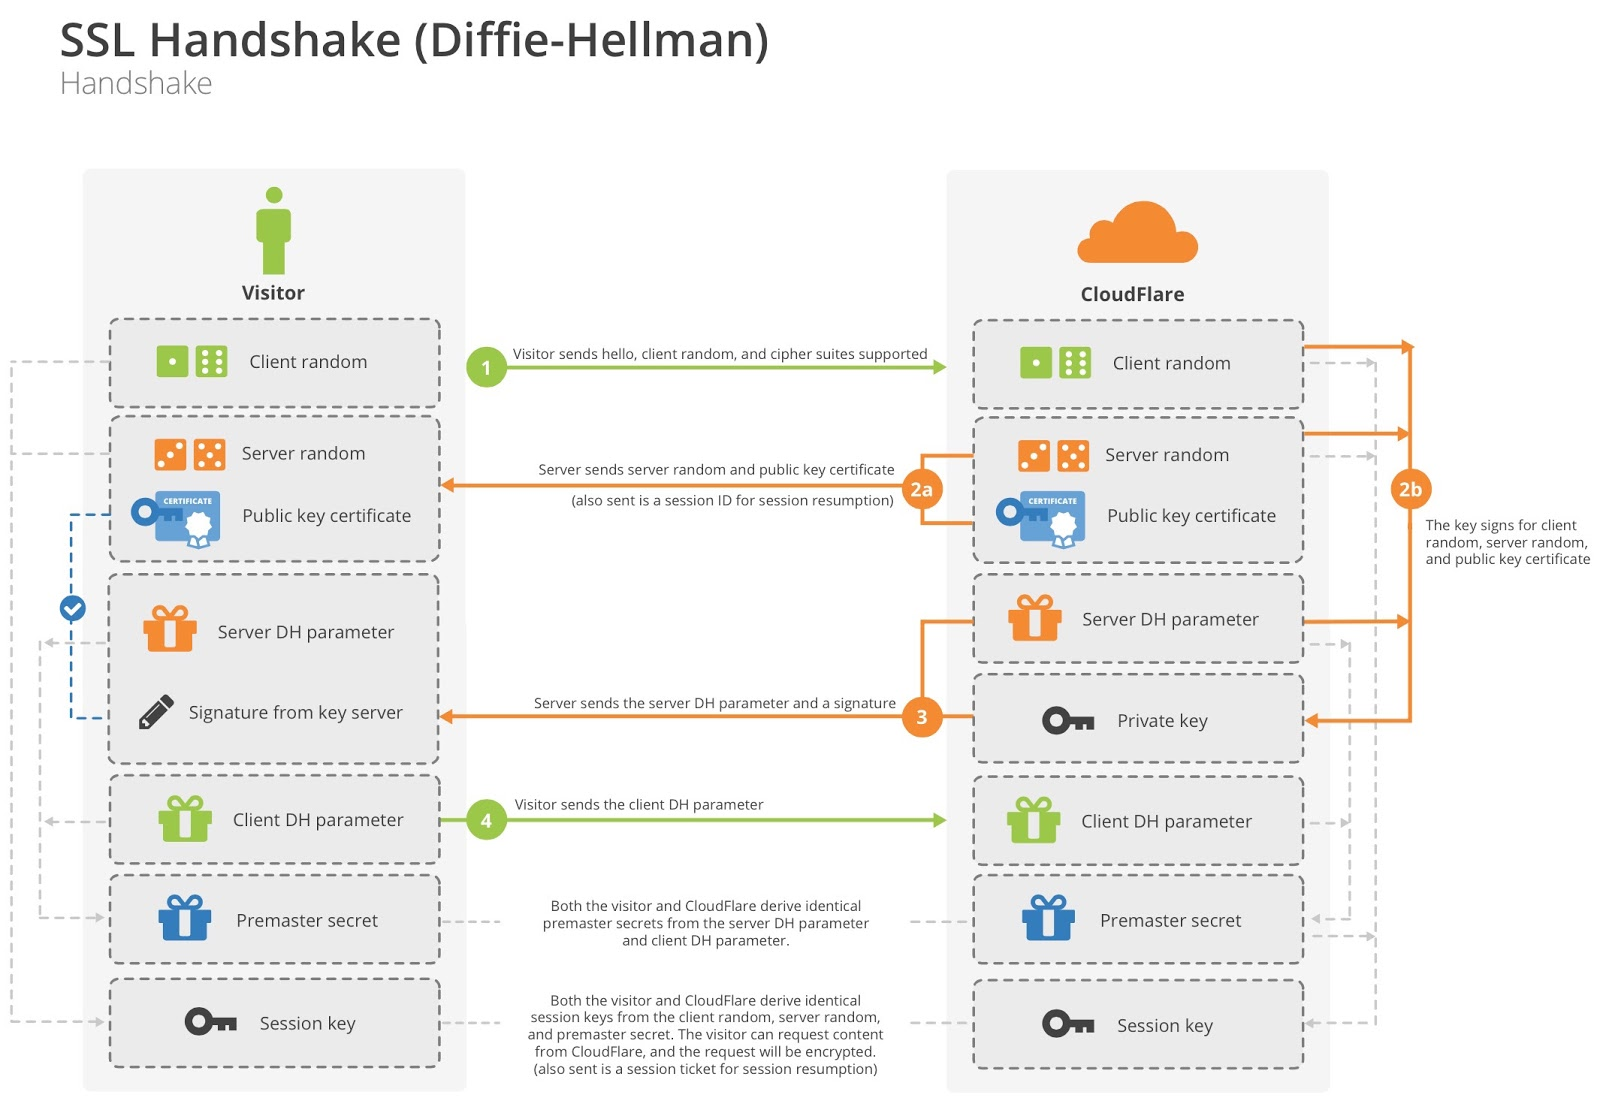
\includegraphics{./assets/figures/TODO_pdaas_component-composition_monolithic.jpg}
\caption{PDaaS Architecture, monolithic
composition\label{fig:composition-monolithic}}
\end{figure}

\begin{figure}
\centering
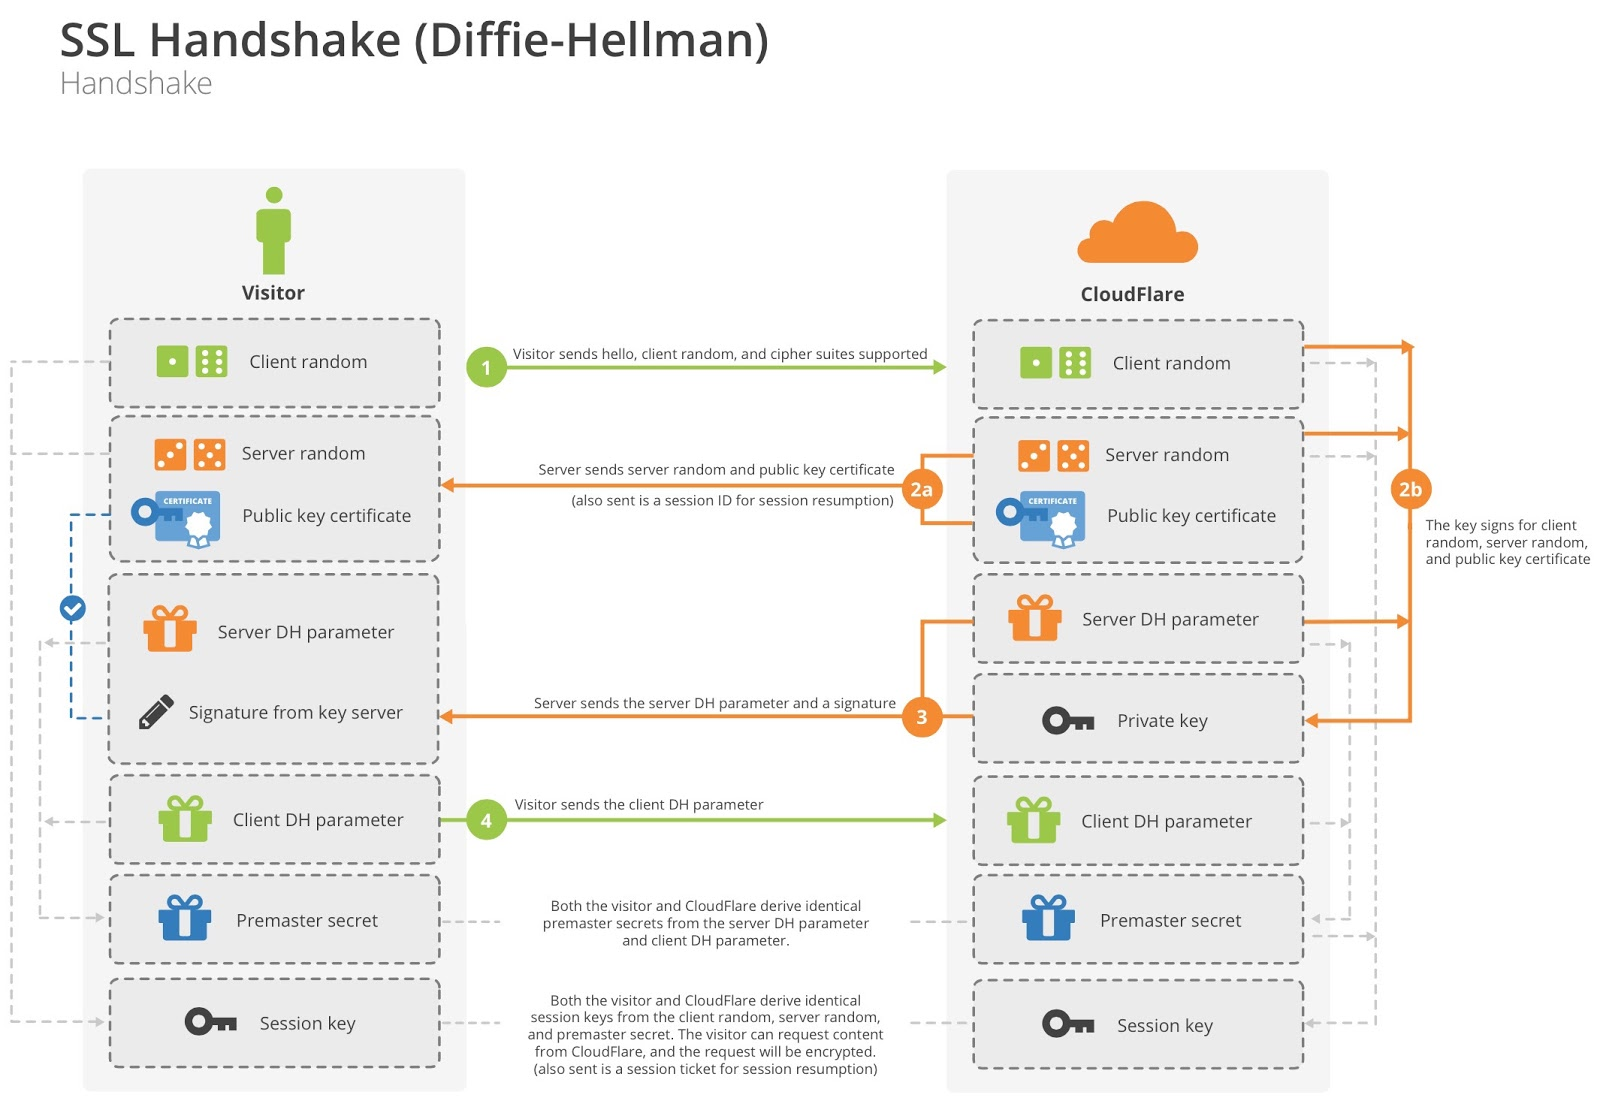
\includegraphics{./assets/figures/TODO_pdaas_component-composition_distributed.jpg}
\caption{PDaaS Architecture, distributed
composition\label{fig:composition-distributed}}
\end{figure}

The main difference between the two compositions is the lack of the
mobile platform in the more monolithic approach (Figure
\ref{fig:composition-monolithic}). Although \emph{monolithic} refers
only to the components arrangement on the \emph{server} platform. It is
also imaginable that all server components not necessarily have to be
placed into one server environment, but being distribute over several
virtual machines or containers, so that they can scale and run more
independently. This can improve \emph{redundancy} as well.

In theory, a possible version of the arrangement would be to move all
components to either the desktop or the mobile platform. This comes
along with some downsides and major issues that are anything but trivial
to solve. Aside from ensuring a nearly 100\% uptime and localization in
a landscape where NAT\footnote{Network Address Translation; practice of
  routing traffic between and through distinct networks address spaces
  by remapping IPs from those different networks onto each other} and
dynamic IPs are still common practice, not only on the mobile platform
but on the desktop platform as well, all component, but the user
interface, needs to be implemented with native technologies.
Nevertheless, from a \emph{operator's} perspective it would mean having
all components at hand and therefore full control over the \emph{PDaaS},
it still would lack of major requirements, though.

Aside from providing the \emph{operator} with a non-stationary and
instantly accessible interface to her \emph{PDaaS}, involving a
\emph{mobile platform} has the purpose of enabling the \emph{data
subject} to carry all her sensitive data along. This is considered a
major advantage over the monolithic approach, were all the personal data
is located in the \emph{``cloud''}. Depending on the perspective, it can
either be seen as a \emph{singe source of truth} or a \emph{single point
of failure}. Regardless of that, it introduces the demand of a backup or
some redundancy concept, which has briefly been touched on in the
discussion about database system requirements within the
\protect\hyperlink{data}{\emph{data} section}. A mobile platform being
part of the system makes it more easier for the \emph{data subject} to
establish a security concept, in which the relation the between personal
data storage and the rest of the system is much more liberated, so that
all access attempts only happen under full supervision. It is debatable
whether to place the \emph{permission profiles} in the \emph{persistence
layer} among all other domain-related information, or put it into the
\emph{personal data storage} as well or define it as an own storage
component, in order to be flexible regarding it's location.

Authenticating \emph{consumers} is performed based on TLS by the web
server and it's configured subdomains including their individual keys
and certificates provided by the \emph{PKI}. The \emph{operator}
authentication is either done by the \emph{Operator API} or by the
\emph{web server}, depending on the \emph{web server's} capabilities.
Though, it makes more sense, to entrust the \emph{web server} with that
task, because it's the outmost component and it would prevent
unauthorized and potential malicious requests from getting further into
the system. And since a native front end on a mobile platform is
considered \emph{private}, it is reasonable to change the
\emph{operator} authentication from JWT-based to TLS-based \emph{two-way
authentication}, which would otherwise be inconvenient when using
web-based front ends.

If there are components that are only placed on the server and that have
to communicate between each other, but are separated into independent
processes, then some inter-process communication need to be established
(e.g.~sockets). It is also conceivable that inter-communication between
server components could be unidirectional only. Approaches like changing
configuration files by writing to the filesystem can therefor be
feasible in some cases. Components that can vary in terms of their
platform, have to communicate to the other components via \emph{HTTPS}.

The architecture implicitly distinguishes between two different groups
of endpoints. These endpoints are made available by the \emph{web
server}, which reverse-proxys incoming connections to role-related
(\emph{operator} or \emph{data consumer}) components. Starting from
that, this separation can be driven further by simply encapsulating
those components into services, that either are related to one of the
roles or used by both. This basically results in the \emph{web server}
communicating with the two role-services in a bidirectional manner. The
group of endpoints for \emph{data consumers} mainly consists of those
were \emph{access requests} and \emph{permission requests} are coming in
and the public one, that is used for \emph{consumer} registrations. The
other one is a small group of endpoints required for all the tools the
\emph{operator} might need; from data API or notification through to
authentication and web-based user interface.

Considering the rapid growth of emerging website and applications, which
all require user registration, users are getting tired of creating new
accounts. Hence they tend to reuse their password(s). Providers started
outsource that sensitive topic of user management by integrating third
party authentication services, which not only makes is almost effortless
to implement, but also leaves the responsibility as well as the
accessibility to those service owners. Whereas users get the benefit of
just using one account for all her apps - a universal key so to say, but
only one exemplar. So the downside here is, only a handful of third
parties
{[}\protect\hyperlink{ref-web_2009-success-of-facebook-connect}{133}{]}
provide those authentication services.\\
OpenID is designed with a very specific type of scenarios in mind,
namely the one just described - bringing decentralisation to the market
of authentication services - which differs from those addressed by the
\emph{PDaaS}; at least, when it comes to \emph{data consumer}
interactions. Although, the \emph{PDaaS} has the ability to become the
digital representation of it's \emph{operator}. Hence it can and also
should be used to authenticate that individual against an external
parties.

\emph{\textbf{Conclusions:}} Considering amount of effort a
single-platform version, namely desktop or mobile, would take to get
fully operational with respect to the specification, it is not only
reasonable but also more secure to involve a server environment with
proper security measures, static IP and high availability. Even if that
server is a local machine connected to the \emph{data subject's} private
network. That said, it is sufficient to start with the \emph{monolithic}
approach and as suitable mobile applications emerge that are supporting
major administration features, notifications and \emph{personal data
storage}, it should be possible to migrate effortlessly towards the
\emph{distributed} approach that comes with a higher level , because all
the sensitive personal data somewhere on a computer machine. As of the
proposed architecture all components (or group of components) are
portable and therefore relocatable among the suggested platforms; and
with the introduced authentication method for \emph{operators} using
multiple front ends for the same \emph{PDaaS} are thereby supports and
can be implemented with almost no effort, which covers more use cases.
As a supplement, an \emph{identity provider} based on the OpenID
standard would fit nicely into the existing arrangement and not
interfering with the other components. However, it is beyond the scope
of this work to make elaborate on this topic. For now it is stated as a
feasible and logical addition to the \emph{PDaaS}.

\section{Environment and Setup}\label{environment-and-setup}

As stated in the project's core principles \emph{Open Development} is
vital for the project to gain trust. Interestingly, this has a
significant impact on how a \emph{PDaaS} might be deployed or installed.
All its components can just get taken and used as it suits everyone's
needs; of cause, while respecting their licenses. Furthermore, enforcing
\emph{portability} leads to a more simplified and independent
development process that can be organized in a way so that the primary
division into components can be leveraged.

The range of environment systems for \emph{server} platforms is highly
diverse but the main shares belong to either the UNIX or LINUX family,
even though almost every platform is POSIX-compliant.\footnote{Portable
  Operating System Interface; a collection of standards released by the
  IEEE Computer Society to preserve compatibility between operating
  systems.} When it comes to \emph{mobile} platforms the market is fare
less divers. Native applications are either developed in \emph{Java}
(for Google's Android) or in Swift (for Apple's iOS). Whereas the
environment systems has nearly no relevance for the \emph{desktop},
other then the screen size and maybe which browser and version the
environment system runs. But that's probably something the user can
change.

As a result, being able to use certain components on a \emph{server}
platform depends on what \emph{server} environment is provided. And vice
versa, in order to decide on what implementation of a component is
suitable, it's crucial in what environment that component has to run in.
Either way, not to forget all the dependencies a component might have.
Such constraints can be avoided by abstracting the runtime of those
components and either embed every required software dependency or
provide them in separate runtimes, if that's possible. Depending on the
technologies used, this concept is commonly known as
\emph{virtualization} or \emph{containerization}. It isolates software
by putting them into so called \emph{container}. But since those
container-wrapped components still have to interact with each other,
they need to be supervised or at least managed. This is done by an
orchestration software, which not only allocates system resources but
also emulates a whole network infrastructure (e.g.~DNS, TCP/IP,
routing). Thereby, it is used to determine how certain container (and
its containing component) are allowed to communicate and what resource
are accessible from inside (e.g.~filesystem). This complete abstraction
to the surrounding environment means it quasi is the only dependency the
\emph{PDaaS} would have, regardless of how its components are
implemented. They just have to be \emph{``containerizable''} - satisfy
the \emph{\protect\hyperlink{link-container}{container image
specification}} {[}\protect\hyperlink{ref-web_oci-spec_image}{107}{]}.
This concept can be utilized for the
\emph{\protect\hyperlink{supervised-data-access}{supervised code
execution}} (\protect\hyperlink{sa01}{S.A.01}) mentioned before without
any restraints.

Migrating from a server-located \emph{personal data storage} to the
\emph{mobile} based version introduces another challenge. The subsequent
approach is a first and more general solution to that problem.

\emph{NOTICE: it is assumed that a running instance of a }PDaaS* is in
place, the \emph{operator} owns a modern mobile device and on this
device a \emph{PDaaS} mobile application is installed.*

\begin{enumerate}
\def\labelenumi{\arabic{enumi}.}
\item
  After starting the app, the \emph{operator} needs to establish a
  connection between the server and mobile application. Therefor the
  \emph{operator} either has to scans a QR-Code with the help of that
  app. THe QR-Code is presented to the \emph{operator} within her
  personal management interface of the \emph{PDaaS} running in a
  browser. Or the \emph{operator} inserts her credentials in to a form
  presented by the mobile application.
\item
  After the connection has established, the \emph{operator} can trigger
  a progress that duplicated all her \emph{personal data} to the device
  that just has been associated with the \emph{PDaaS}.
\item
  At this point one of two ways can be proceeded, depending on whether a
  complete write log for the \emph{personal data}
  (\protect\hyperlink{data}{see discussion about backup strategies} does
  exist or not.

  \begin{enumerate}
  \def\labelenumii{\alph{enumii})}
  \tightlist
  \item
    \emph{{[}LOG-EXISTS{]}} query by query the whole log is obtained
    from the existing storage and is then again executed in
    chronologically order by the query language abstraction. The only
    difference here is that the target storage,on which that query is
    actually performed on, is located on that newly introduced platform
  \item
    If the \emph{{[}LOG-NOT-EXISTS{]}}, the situation is more
    complicated, if the database systems are not based on exactly the
    same technology. Hence, additional migration software is required.
    If both database systems provide import and export mechanisms that
    support at least one interoperable data format, the migration
    software can leverage this features simply by exporting all the data
    and saving it to the filesystem. The software then transfers dump to
    the target environment and triggers the import process. Otherwise,
    the software not only needs to be aware of both database systems and
    their native query, it also has to have a comprehensive
    understanding of how their data structuring concepts work, in order
    to reliably transform one into the other. So to be more specific, at
    first the software has to analyse the structure of source database.
    Based on this result it might need to perform some configuration on
    the target database, before actually obtaining the data from the
    source database. The received data then need to be transformed into
    queries that are supported by the target system. Those transformed
    queries are transferred to the target environment, where those
    incoming queries get executed until all data is migrated.
  \end{enumerate}
\item
  After thr duplication process has finished, the \emph{operator} can
  decide which \emph{PDS} the \emph{PDaaS} should use to serve
  \emph{access requests} and what should happen with the other
  storage(s).
\end{enumerate}

So to conclude, a migration process of moving \emph{personal data} from
one platform instance to another can be much more simplified and robust,
if a complete query log would exist. It is also worth mentioning, that
the migration process described above is not restricted to exactly this
source or migration direction. As long as target and source are either a
\emph{server} or a \emph{mobile} platform, any variant is imaginable.

\emph{\textbf{Conclusions:}} Installing a \emph{PDaaS} should be
straightforward with the least possible effort being used for
preparations. Package manager of all popular operating systems should
offer (semi-)automated installations. Additionally, components
themselves and the project as whole have to provide detailed
documentations for various ways of how those parts or the entire system
need to be installed. Alternatively, \emph{data subjects} might be are
willing to entrust external third parties with hosting a \emph{PDaaS}
instance for them. In that case the distributed approach involving a
\emph{mobile} platform might come in handy, so that the actual data is
not stored somewhere beyond their reach. THe \emph{PDaaS} as an open
source development encourages anybody who is interested or even wants to
contribute to checkout the source code of the various implementations,
get it to run and play around with it. But for that at least the
components of the \emph{server} platform are required to have documented
on what other software they depend on, so that the target environment
can be prepared accordingly. Aside from hardware on which the
\emph{PDaaS} needs to run, the only other requirement is owning a
internet domain that is registered on a public DNS\footnote{Domain Name
  System; decentralized open directory that associates readable names
  with IP addresses} server and has no subdomains configured yet.

If a component needs to get segregated from its host environment,
\emph{containerization} is the recommended technique, since it causes
less overhead compared to \emph{virtualization} and is generally a
lightweight approach. Though, additional abstraction might also
introduce new problems instead of solving them.

\section{User Interfaces}\label{user-interfaces}

Designing graphical user interfaces is beyond the scope of this work and
the \emph{PDaaS} specification as well. Nevertheless this section shell
be understood as a collection of proposed ideas addressing the questions
of what types of user interfaces the \emph{PDaaS} should provide and
which features they might need to support.

The most notable characteristic used to distinguish user interfaces from
each other are those interfaces that are visible and the ones that
arn't. For example a \emph{graphical user interface (GUI)}, composed of
visually separated areas with a certain semantic and assembled with
meaningful objects on which the user can physically act, for example by
touching them. The interface then reacts on those actions by changing
their appearance. In this way the user can comprehend her actions.
Whereas non-graphical user interfaces don't provide the user with
objects or surfaces to interact with. Instead, the primarily used medium
is text, regardless if it's human-readable or not. But \emph{command
line interfaces (CLI)}, available mainly in command line environments or
shells, still provides a certain level of interactivity. A running
program can pause in order to prompt the user with an input request. If
an input is made and submitted the program then proceeds. The group of
interfaces whose interactions can be fully automated are for example
\emph{application programming interfaces (API)}. Depending on the
transport technologies, it's no unusual that \emph{API} interactions are
consisting of just one action causing one reaction. Non-graphical
interfaces enabling interactions on lower level. Even though they
provide more functionality and can more time efficient, they are more
rudemental and often less secure. While \emph{GUIs} are normally meant
for end users to interact with applications on a more sophisticated
level, \emph{CLIs} are used during development, for automation, or for
server environment administration; probably remotely, because they are
typically headless. Whereas \emph{APIs}, documented by its provider,
used to enable software developers program automated requests against
those interfaces.

Table \ref{tbl:ui-features} provides a list of features and associates
the different user interfaces mentioned before to those features if they
should be supported by the interface types. It is notable that the
\emph{GUI} provides the \emph{operator} with a powerful tool Hence it
requires reliable protection mechanisms (see
\protect\hyperlink{authentication}{Authentication}). Whereas \emph{API}
capabilities are very limited, because it's the one interface that the
\emph{PDaaS} exposes to third parties.

\begin{longtable}[]{@{}lccc@{}}
\caption{Features that should be supported by the given user interfaces
\label{tbl:ui-features}}\tabularnewline
\toprule
Feature & GUI & CLI & API\tabularnewline
\midrule
\endfirsthead
\toprule
Feature & GUI & CLI & API\tabularnewline
\midrule
\endhead
manage \emph{permission profiles} (\protect\hyperlink{pviu03}{P.VIU.03})
& \textbf{X} & - & \textbf{X}\tabularnewline
view access history (\protect\hyperlink{pviu04}{P.VIU.04}) & \textbf{X}
& \textbf{X} & -\tabularnewline
register \emph{consumer} & \textbf{X} & \textbf{X} & -\tabularnewline
add new \emph{front end} & \textbf{X} & - & -\tabularnewline
authenticate \emph{operator} & \textbf{X} & - & -\tabularnewline
migrate \emph{personal data} & \textbf{X} & \textbf{X} &
-\tabularnewline
review \emph{permission requests} (\protect\hyperlink{pi04}{P.I.04}) &
\textbf{X} & - & -\tabularnewline
create \& maintain templates (\protect\hyperlink{pi05}{P.I.05}) &
\textbf{X} & - & -\tabularnewline
adjust precision of data (\protect\hyperlink{pi06}{P.I.06}) & \textbf{X}
& - & \textbf{X}\tabularnewline
introduce new data \emph{structs} & \textbf{X} & - &
\textbf{X}\tabularnewline
configure \emph{PDaaS} & \textbf{X} & - & -\tabularnewline
import personal data & \textbf{X} & - & \textbf{X}\tabularnewline
read/access \emph{personal data} & \textbf{X} & \textbf{X} &
\textbf{X}\tabularnewline
manipulate \emph{personal data} & \textbf{X} & \textbf{X} &
-\tabularnewline
run supervised code execution & - & \textbf{X} &
\textbf{X}\tabularnewline
\bottomrule
\end{longtable}

The architectural design includes \emph{desktop} and \emph{mobile}
platforms. While prioritizing a web-based \emph{GUI}, the management
tool for the \emph{operator} also need to be implemented natively for
common mobile systems (\protect\hyperlink{pviu02}{P.VIU.02}); in this
case Android and iOS. This again enables to provide real-time
notifications (\protect\hyperlink{pi03}{P.I.03},
\protect\hyperlink{pb02}{P.B.02}) on mobile platforms, whereas
WebSocket-based connections add this feature to \emph{desktop}
platforms. Since screen sizes can vary, in particular on \emph{mobile}
platforms, the \emph{GUI} is required to be highly responsive and has to
adapt (\protect\hyperlink{pviu01}{P.VIU.01}). Given the capabilities of,
a inaccurate or error-prone rendered \emph{GUI} can quickly cause
unintended incidents. The main focus though has to

Known challenges for the \emph{GUI} design are primarily developing very
efficient but also fun to use interfaces for reviewing \emph{consumer
registrations} and \emph{permission requests}. Especially the latter can
become hard to solve, because how can graph-based and nested data
structures be displayed in such a way that makes reviewing and also
manipulating an easy task to do - even on a screen of a mobile phone.
One approach could be to utilize the \emph{accordion} pattern
{[}\protect\hyperlink{ref-web_2016_wikipedia_accordion-gui}{134}{]} for
edges and start nesting them in order to represent subsequent data
structure. The interaction then might look like tree-structured
navigation moving along relations just by expanding and folding in data
points.

Since other parts of the system have to provide the mechanisms to
increase or reduce the precision of data due to privacy protection, the
challenge here is to find the right design concepts for \emph{data
subject} to facilitate those adjustments. Precision adjustments can be
achieved by either changing the sampling rate in a dataset containing a
series of data points, or by rounding values to a certain extend. An
example is cutting fractional digits of the latitude and longitude
values in a position information, or removing all position information
obtained between every quarter from a full day tracking period. Whether
\emph{data subjects} can choose from an abstracted precision grading
(e.g. \emph{high}, \emph{mid}, and \emph{low}) or they set specific,
type or unit related filter mechanisms, configurable defaults on a
system-wide level should be provided by \emph{GUIs} in any case.
Following data types are supposedly vulnerable to compromise privacy,
thus proposed to support precision adjustments: \emph{Date} (time), any
kind of absolute measurements, sets containing data series, and position
information, as mentioned before.

\emph{\textbf{Conclusions:}} The most important aspect, when interacting
with something or someone, is being provided with some kind of feedback.
An action typically causes - and is therefore expected - a reaction. The
result is an interaction, unless no reaction occurred.

The discussion above outlines the relevance of those interactions for
the \emph{PDaaS}. Thus, for users and other software to interact with
the \emph{PDaaS} interfaces are mandatory. Primary characteristics of
those interfaces are complete functionality, security precautions and
restrictions, as well as comprehensive documentations. And visual user
interfaces in addition, need to provide reliable and adaptive rendering,
a consistent and encouraging interaction design and. \emph{GUIs} need to
be provided for all \emph{desktop} and \emph{mobile} platforms,
primarily to provide an efficient user experience for the
\emph{operator}. The \emph{operator} is the only role with permissions
to access a \emph{GUI}. Components on the \emph{server} platform should
provide \emph{CLIs}, at least when no other technical option exist to
interact with them. Also accessing the database from command line could
be appreciated at some point. \emph{APIs} are mostly meant for
\emph{data consumers} to interact with the \emph{PDaaS} and perhaps for
automated data contribution (based on \emph{operator} role; e.g.~browser
plugin). \emph{Desktop} platforms might use those \emph{APIs} as well.
In any case, \emph{APIs} must be separated according to the
\emph{roles}.

These are all vital characteristics whose details need to be addressed
by the \emph{specification}. Whose implementation details though are not
the concern of this specification, as long as every stated requirement
is being acknowledged.

\chapter{\texorpdfstring{Specification
\emph{(Draft)}}{Specification (Draft)}}\label{specification-draft}

This chapter hold the first draft of what might become a specification.
As for now it has therefore no claim of completeness, continuity or
accuracy. The contents is based on and a result of all previous
discussions and developed solutions.

TODO: should might must n stuff in table (see dark mail spec)

\section{Overview}\label{overview}

\begin{itemize}
\tightlist
\item
  purpose
\item
  architectural overview
\item
  short description of the whole process
\end{itemize}

\section{Components}\label{components}

\subsection{Webserver}\label{webserver}

\subsection{User Interface}\label{user-interface}

\subsection{Storage/Persistence}\label{storagepersistence}

\subsection{Notification
Infrastructure}\label{notification-infrastructure}

\subsection{Data API}\label{data-api}

\section{Data}\label{data-1}

\subsection{Structure \& Types}\label{structure-types}

\begin{itemize}
\tightlist
\item
  henceforth only two things: primitive and struct
\item
  supported date types
\end{itemize}

\subsection{Read}\label{read}

\subsection{Write}\label{write}

(!) every data or configuration change has to be reversible

precision of data: demanding lower precision than the \emph{data
subject} has approved is always possible. The other ways around not.

\section{Protocols}\label{protocols}

\subparagraph{Consumer registration}\label{consumer-registration}

\begin{enumerate}
\def\labelenumi{\arabic{enumi})}
\setcounter{enumi}{-1}
\item
  {[}OPTIONAL{]} \emph{data subject} provides URI to \emph{data
  consumers}
\item
  \emph{data consumers} create \emph{permission request} that includes

  \begin{itemize}
  \tightlist
  \item
    X.509 based CSR\footnote{Certificate signing request}
  \item
    callback URI via HTTPS as feedback channel
  \item
    {[}OPTIONAL{]} information about what data points wanted to be
    accessed
  \end{itemize}
\item
  depending on 0), \emph{data consumer} provides \emph{operator} with
  priorly created \emph{permission request} either as QR-Code or via
  HTTPS by given URI
\item
  \emph{operator} reviews request and decides to either refuse or grant
  assess; the latter results in:

  \begin{enumerate}
  \def\labelenumii{\alph{enumii})}
  \tightlist
  \item
    creating new \emph{endpoint}

    \begin{itemize}
    \tightlist
    \item
      create new unique subdomain and a related asymmetric key pair
      signed by the system's root CA (self-signed)
    \item
      issue \emph{consumer} certificate based on it's CRS and sign it
      with the key pair related to this \emph{endpoint}
    \end{itemize}
  \item
    if information is provided, creating new \emph{permission profile}
    by either applying existing draft/template or configuring
    \emph{permission type} (incl. expiration date if required) and
    permitted data endpoints; associate to specific \emph{endpoint}
  \end{enumerate}
\item
  \emph{data consumers} gets informed about the decision via callback
  channel

  \begin{itemize}
  \tightlist
  \item
    on grant, response includes

    \begin{itemize}
    \tightlist
    \item
      \emph{consumer's} certified certificate
    \item
      certificate that's associated with the created endpoint
    \item
      information on what data points are allowed to be accessed;
    \end{itemize}
  \item
    on refusal: error code/message
  \end{itemize}
\item
  \emph{data consumer} handles the response appropriately

  \begin{itemize}
  \tightlist
  \item
    {[}OPTIONAL{]} pin the provided \emph{PDaaS} certificate
  \end{itemize}
\end{enumerate}

\subparagraph{Data Access}\label{data-access}

\begin{enumerate}
\def\labelenumi{\arabic{enumi})}
\setcounter{enumi}{-1}
\item
  after successfully authenticated, \emph{consumer} sends \emph{access
  request}
\item
  request contains at least the \emph{data query}; based on that query
  and the \emph{permission profiles}, access is tried to get verified

  \begin{enumerate}
  \def\labelenumii{\alph{enumii})}
  \tightlist
  \item
    on success, response gets computed
  \item
    on failure, error code/message is responded; process aborts

    \begin{itemize}
    \tightlist
    \item
      if the error was raised because no appropriate \emph{permission
      profile} was found, then the \emph{consumer} first needs to
      request permission for the \emph{data points} that were part of
      the query
    \end{itemize}
  \end{enumerate}
\item
  {[}OPTIONAL{]} depending on whether the \texttt{keepalive} flag was
  set \texttt{true}, the connection of this requests lasts until
  response computation has finished or timeout has reached, otherwise
  the response contains a URI unique to this current request including
  an estimation when response will be available under that URI;
  connection can still timeout, which is defined by the system
\item
  depending on the type of that \emph{access request},

  \begin{enumerate}
  \def\labelenumii{(\Alph{enumii})}
  \tightlist
  \item
    the data get queried and the result is added to the response
  \item
    based in further information provided by the request, the
    environment for the \emph{supervised code execution} is getting
    provisioned, the program from the \emph{consumer} will be ran
    against various tests

    \begin{enumerate}
    \def\labelenumiii{\alph{enumiii})}
    \tightlist
    \item
      in fail, error code/message get added to the response
    \item
      on pass, computed result gets added to the response
    \end{enumerate}
  \end{enumerate}
\item
  response is finalized and gets returned back to the \emph{consumer},
  either as a response to this request or provided under the unique URI
  as of 2)
\end{enumerate}

\subparagraph{Permission Validation}\label{permission-validation}

TODO: detailed description of the algorithm that checks \emph{permission
profiles} according to an \emph{access request}; including all different
possible cases (multiple profiles for one consumer etc)

\subparagraph{Add or Change Personal
Data}\label{add-or-change-personal-data}

\subsection{Data Management}\label{data-management}

\begin{itemize}
\tightlist
\item
  one third party access (consumer) relates to one access
  \emph{endpoint}, that also authenticates that third party by TLS based
  \emph{two-way auth}
\item
  zero or more \emph{permission profiles} are associated to one
  \emph{endpoint}
\end{itemize}

\section{APIs}\label{apis}

\textbf{Registration Request}

\begin{itemize}
\tightlist
\item
  contains certificate signing request
\item
  {[}OPTIONAL{]} contains \emph{permission request}
\end{itemize}

\begin{Shaded}
\begin{Highlighting}[]
\FunctionTok{\{}
    \DataTypeTok{"callbackUri"}\FunctionTok{:} \StringTok{"TODO"}\FunctionTok{,}
    \DataTypeTok{"csr"}\FunctionTok{:} \StringTok{"TODO"}\FunctionTok{,}
    \DataTypeTok{"dataPoints"}\FunctionTok{:} \OtherTok{[}
        \StringTok{"profile.lastname"}
    \OtherTok{]}
\FunctionTok{\}}
\end{Highlighting}
\end{Shaded}

\textbf{Permission Request}

\begin{itemize}
\tightlist
\item
  creates new \emph{permission profile}
\item
  \texttt{https://example-consumer.pdaas.tld/pr}
\end{itemize}

\begin{Shaded}
\begin{Highlighting}[]
\FunctionTok{\{}
    \DataTypeTok{"callbackUri"}\FunctionTok{:} \StringTok{""}\FunctionTok{,}
    \DataTypeTok{"dataPoints"}\FunctionTok{:} \OtherTok{[}
        \StringTok{"profile.lastname"}
    \OtherTok{]}
\FunctionTok{\}}
\end{Highlighting}
\end{Shaded}

\textbf{Access Request}

\begin{itemize}
\tightlist
\item
  obtains actual data
\item
  if \texttt{keepalive} is set \texttt{true}, the connections lasts
  until response computation has finished, otherwise the response
  contains a URI unique to this current request including an estimation
  when response will be available under that URI; connection can still
  timeout, which is defined by the system
\item
  \texttt{https://example-consumer.pdaas.tld/ar}
\end{itemize}

\begin{Shaded}
\begin{Highlighting}[]
\FunctionTok{\{}
    \DataTypeTok{"query"}\FunctionTok{:} \StringTok{"TODO"}
\FunctionTok{\}}
\end{Highlighting}
\end{Shaded}

\emph{Requirements:}

\begin{itemize}
\tightlist
\item
  query has to match exactly one corresponding \emph{permission profile}
\end{itemize}

TODO: basic structure of a \emph{permission profile}

How do the APIs involved with the protocols look like?

\section{Security}\label{security}

\begin{itemize}
\item
  the downside of having not just parts of the personal data in
  different places (which is currently the common way to store), is in
  case of security breach, it would increase the possible damage by an
  exponential rate Thereby all data is exposed at once, instead of not
  just the parts which a single service has stored
\item
  does it matter from what origin the data request was made? how to
  check that? is the requester's server domain in the http header?
  eventually there is no way to check that, so me might need to go with
  request logging and trying to detect abnormal behaviour/occurrence
  with a learning artificial intelligence
\item
  is the consumer able to call the access request URI repeatedly and any
  time? (meaning will this be stateless or stateful?)
\item
  initial consumer registration would be done on a common and valid
  https:443 CA-certified connection. after transferring their cert to
  them as a response, all subsequent calls need to go to their own
  endpoint, defined as subdomains like
  \texttt{consumer-name.owners-notification-server.tld}
\end{itemize}

\subsection{Environment}\label{environment}

\subsection{Transport}\label{transport}

\begin{itemize}
\tightlist
\item
  communication between internal components \emph{must} be done in https
  only, but which ciphers? eventually even http/2?
\end{itemize}

\subsection{Storage}\label{storage}

\begin{itemize}
\tightlist
\item
  documents based DB instead of Relational DBS, because of
  structure/model flexibility
\item
  graphql because of it's nature to abstract a storage engine, which
  comes in handy when the actual storage gets relocated (e.g.~from a
  server to a mobile device)
\end{itemize}

\subsection{Authentication}\label{authentication-1}

\begin{itemize}
\tightlist
\item
  how should consumer authenticate?
\end{itemize}

\section{Recommendations}\label{recommendations}

\subsection{Software Dependencies}\label{software-dependencies}

\subsection{Host Environment(s)}\label{host-environments}

\chapter{Conclusion}\label{conclusion}

\section{\texorpdfstring{Ethical \& Social Impact (TODO: or
``Relevance'')}{Ethical \& Social Impact (TODO: or Relevance)}}\label{ethical-social-impact-todo-or-relevance}

\begin{itemize}
\item
  Regarding involving an official party to verify data reliability: The
  actual question would be, is the \emph{data subject} certain, that she
  really wants to hand over those capabilities to official authorities?
  Depending on which \emph{data consumers}, what task their are
  entrusted with and what motivation the \emph{data subject} has has in
  mind to do so, the \emph{PDaaS} might become a powerful
  \emph{``digital reflection''} and starts to get seen as a real and
  reliable representation of herself. Then the decisions made by
  \emph{data consumers} might have a big impact for the \emph{data
  subject's} life. For example a housing loan won't be granted or a
  medical treatment has been refused.
\item
  give back the data subject to control the level of privacy she is
  willing to share
\end{itemize}

\section{Business Models \&
Monetisation}\label{business-models-monetisation}

\begin{itemize}
\tightlist
\item
  possible resulting direct or indirect business models
\item
  data subject might want to sell her data, only under her conditions.
  therefor some kind of infrastructure and process is required (such as
  payment transfer, data anonymization, market place to offer data)
\end{itemize}

\section{Target group perspectives}\label{target-group-perspectives}

\begin{itemize}
\tightlist
\item
  User: would I use this stuff? The underpinning technical details and
  how it works is not my concern and non of my interests. I want this
  stuff work and being reliable. it its simple to use. and maybe even
  easy to setup (server n stuff), then the hell, I would!
\item
  Dev:

  \begin{itemize}
  \tightlist
  \item
    spec implementer
  \item
    integrater in consumer:
  \end{itemize}
\item
  Consumer:

  \begin{itemize}
  \tightlist
  \item
    what can she do with it: adjsut precision of datasets and values to
    increase privacy
  \item
    control and get an overview on where her data might flow (and for
    what purpose)
  \end{itemize}
\end{itemize}

TODO: make a reference or involve the research mentioned at the
beginning

\section{Challenges}\label{challenges}

\begin{itemize}
\item
  adoption rate of such technology
\item
  data reliability from the perspective of a \emph{data consumer} Since
  it is almost impossible to ensure complete reliability of all the data
  a \emph{PDaaS} has stored or might me offering, and because it is
  operated by exactly that individual, and that individual only, all
  data in question is relates to and is thereby owned by her, it, of
  cause, makes it not easy for \emph{data consumers} to trust
  \emph{PDaaS}s as resources for their business processes, but I am
  certain, that the demand for all different kinds of data exceeds the
  partial uncertainty of their reliability.
\item
  personal data leaking Preventing personal data from being leaked to
  the outside, is, especially because of the system's purpose, extremely
  hard to prevent, if not possible at all. Just by querying data from
  the storage or by physically transferring them from one location to
  another, it's already copied. It's the very nature of digital
  information technology/systems. So this cannot be defeated. It only
  can be impeded. Interestingly though, is the same approach the media
  industry for centuries is trying to make copyright infringements more
  difficult.
\item
  scenario where the mobile device, or in general the data storage get
  lost. first of all, not much of a problem, because either device
  backup or since the liberal relation, the system would continue to
  function, but limited, until a data storage gets part of the system
  again (TODO: touched on in the data section at the end)
\item
  during concept development, it appears to become necessary to define
  another role, for \emph{data contributors} (plugins/clients that are
  authorized by the \emph{operator} but only allowed to push data to the
  \emph{PDaaS}).
\end{itemize}

\section{Solutions}\label{solutions}

\begin{itemize}
\item
  even though \emph{OAuth} don't find it's way into this project,
  working through the standard inspired here and there a solution, for
  example using a URI as a feedback channel or TODO.
\item
  refer to the scenarios at the beginning by saying that with the
  \emph{PDaaS} one is able to implement all of them
\end{itemize}

\section{Attack Scenarios}\label{attack-scenarios}

\begin{itemize}
\item
  single point of failure (data-wise),

  \begin{itemize}
  \tightlist
  \item
    but considering what data users already put into their social
    networks (or: thE social network: fb), they/it has already become a
    de facto data silo and is thus a single point of failure. If that
    service breaks or get down, the data from all users might be lost or
    worse (stolen). The aspect of data decentralisation achieved by
    individual data stores can be valued as positive.
  \end{itemize}
\item
  what about token stealing when using jwt?
\item
  future work: add/activate an intrusion detection system
\end{itemize}

\section{Future Work}\label{future-work}

\begin{itemize}
\item
  maybe enable the tool to play the role of an own OpenID provider?
\item
  going one step further and train machine (predictor) by our self with
  our own data
  (https://www.technologyreview.com/s/514356/stephen-wolfram-on-personal-analytics/)
\item
  finalize first draft of the spec with all core aspect included and
  outlined
\item
  developing based on that a first prototype to find flaws in the spec.
  iterate/repeat
\item
  release 1.0 (spec and example implementation)
\item
  touch on parts that were left blank
\item
  first supporting platforms
\item
  full encryption of the \emph{data storage}
\end{itemize}

\section{Summary}\label{summary}

\begin{itemize}
\tightlist
\item
  main focus
\item
  unique features
\item
  technology stack \& standards
\item
  resources
\item
  the tool might be not a bulletproof vest, but
\end{itemize}

The work will be continued.

\chapter*{Source Code}\label{source-code}
\addcontentsline{toc}{chapter}{Source Code}

\pagenumbering{Roman} \setcounter{page}{6} \pagestyle{plain}

\textbf{\protect\hypertarget{code-01_sparql-query}{}{Code 01: Example
query in SPARQL}:}

\begin{Shaded}
\begin{Highlighting}[numbers=left,,]
\NormalTok{# }\KeywordTok{query} \DecValTok{1}\NormalTok{: obtain }\KeywordTok{the} \FunctionTok{first} \KeywordTok{and} \FunctionTok{last} \NormalTok{name fof }\KeywordTok{data} \NormalTok{subject}
\NormalTok{PREFIX person: <http://pdaas.tld/schemas/person>}

\KeywordTok{SELECT} \NormalTok{$firstname $lastname}
\KeywordTok{FROM} \NormalTok{<https://unique-consumer-endpoint.pdaas.tld/sparql/profile>}
\KeywordTok{WHERE} \NormalTok{\{}
    \NormalTok{$person person}\CharTok{:firstname} \NormalTok{$firstname .}
    \NormalTok{$person person}\CharTok{:lastname} \NormalTok{$lastname .}
\NormalTok{\}}


\NormalTok{# }\KeywordTok{query} \DecValTok{2}\NormalTok{: obtain }\KeywordTok{all} \NormalTok{bank accounts that are available }\KeywordTok{for} 
\NormalTok{# }\KeywordTok{online} \NormalTok{payment}
\NormalTok{PREFIX bank-account: <http://pdaas.tld/schemas/bank-account>}

\KeywordTok{SELECT} \NormalTok{$accountId $bankName $paymentMethod}
\KeywordTok{FROM} \NormalTok{<https://unique-consumer-endpoint.pdaas.tld/sparql/finance>}
\KeywordTok{WHERE} \NormalTok{\{}
    \NormalTok{$bank-account bank-account}\CharTok{:payment}\NormalTok{-method }\OtherTok{"online-service"} \NormalTok{.}
    \NormalTok{$bank-account bank-account}\CharTok{:payment}\NormalTok{-method $paymentMethod .}
    \NormalTok{$bank-account bank-account}\CharTok{:account}\NormalTok{-id $accountId . }
    \NormalTok{$bank-account bank-account}\CharTok{:bank}\NormalTok{-name $bankName .}
\NormalTok{\}}
\end{Highlighting}
\end{Shaded}

\newpage

\textbf{\protect\hypertarget{code-02_sparql-query-results}{}{Code 02:
Results of Code 01 in JSON}:}

\begin{Shaded}
\begin{Highlighting}[numbers=left,,]
\ErrorTok{//} \ErrorTok{result} \ErrorTok{1:}
\FunctionTok{\{}
    \DataTypeTok{"head"}\FunctionTok{:} \FunctionTok{\{}
        \DataTypeTok{"vars"}\FunctionTok{:} \OtherTok{[}
            \StringTok{"firstname"}\OtherTok{,}
            \StringTok{"lastname"}
        \OtherTok{]}
    \FunctionTok{\},}
    \DataTypeTok{"results"}\FunctionTok{:} \FunctionTok{\{}
        \DataTypeTok{"bindings"}\FunctionTok{:} \OtherTok{[}
            \FunctionTok{\{}
                \DataTypeTok{"firstname"}\FunctionTok{:} \FunctionTok{\{}
                    \DataTypeTok{"type"}\FunctionTok{:} \StringTok{"literal"}\FunctionTok{,}
                    \DataTypeTok{"value"}\FunctionTok{:} \StringTok{"Doe"}
                \FunctionTok{\},}
                \DataTypeTok{"lastname"}\FunctionTok{:} \FunctionTok{\{}
                    \DataTypeTok{"type"}\FunctionTok{:} \StringTok{"literal"}\FunctionTok{,}
                    \DataTypeTok{"value"}\FunctionTok{:} \StringTok{"Jane"}
                \FunctionTok{\}}
            \FunctionTok{\}}
        \OtherTok{]}
    \FunctionTok{\}}
\FunctionTok{\}}

\ErrorTok{//} \ErrorTok{result} \ErrorTok{2:}
\FunctionTok{\{}
    \DataTypeTok{"head"}\FunctionTok{:} \FunctionTok{\{}
        \DataTypeTok{"vars"}\FunctionTok{:} \OtherTok{[}
            \StringTok{"accountId"}\OtherTok{,}
            \StringTok{"bankName"}\OtherTok{,}
            \StringTok{"paymentMethod"}
        \OtherTok{]}
    \FunctionTok{\},}
    \DataTypeTok{"results"}\FunctionTok{:} \FunctionTok{\{}
        \DataTypeTok{"bindings"}\FunctionTok{:} \OtherTok{[}
            \FunctionTok{\{}
                \DataTypeTok{"accountId"}\FunctionTok{:} \FunctionTok{\{}
                    \DataTypeTok{"type"}\FunctionTok{:} \StringTok{"integer"}\FunctionTok{,}
                    \DataTypeTok{"value"}\FunctionTok{:} \DecValTok{0905553715}
                \FunctionTok{\},}
                \DataTypeTok{"bankName"}\FunctionTok{:} \FunctionTok{\{}
                    \DataTypeTok{"type"}\FunctionTok{:} \StringTok{"literal"}\FunctionTok{,}
                    \DataTypeTok{"value"}\FunctionTok{:} \StringTok{"A. W. Fritter Institute"}
                \FunctionTok{\},}
                \DataTypeTok{"paymentMethod"}\FunctionTok{:} \FunctionTok{\{}
                    \DataTypeTok{"type"}\FunctionTok{:} \StringTok{"literal"}\FunctionTok{,}
                    \DataTypeTok{"value"}\FunctionTok{:} \StringTok{"online-service"}
                \FunctionTok{\}}
            \FunctionTok{\}}
        \OtherTok{]}
    \FunctionTok{\}}
\FunctionTok{\}}
\end{Highlighting}
\end{Shaded}

\newpage

\textbf{\protect\hypertarget{code-03_graphql-query}{}{Code 03: Example
query in GraphQL}:}

\begin{Shaded}
\begin{Highlighting}[numbers=left,,]
\NormalTok{# URL}\OperatorTok{:} \NormalTok{https}\OperatorTok{:}\CommentTok{//unique-consumer-endpoint.pdaas.tld/graphql}

\NormalTok{query }\OperatorTok{\{}
    \NormalTok{profile }\OperatorTok{\{}
        \NormalTok{firstname}
        \NormalTok{lastname}
    \OperatorTok{\}}
    \AttributeTok{bankAccounts}\NormalTok{(}\DataTypeTok{paymentMethod}\OperatorTok{:} \StringTok{'online-service'}\NormalTok{) }\OperatorTok{\{}
        \NormalTok{accountId}
        \NormalTok{bankName}
        \NormalTok{paymentMethod}
    \OperatorTok{\}}
\OperatorTok{\}}
\end{Highlighting}
\end{Shaded}

~\\
\textbf{\protect\hypertarget{code-04_graphql-query-result}{}{Code 04:
Result of Code 03 in JSON}:}

\begin{Shaded}
\begin{Highlighting}[numbers=left,,]
\FunctionTok{\{}
    \DataTypeTok{"profile"}\FunctionTok{:} \FunctionTok{\{}
        \DataTypeTok{"firstname"}\FunctionTok{:} \StringTok{"Jane"}\FunctionTok{,} 
        \DataTypeTok{"lastname"}\FunctionTok{:} \StringTok{"Doe"}
    \FunctionTok{\},}
    \DataTypeTok{"bankAccounts"}\FunctionTok{:} \OtherTok{[}
        \FunctionTok{\{}
            \DataTypeTok{"accountId"}\FunctionTok{:} \DecValTok{0905553715}\FunctionTok{,}
            \DataTypeTok{"bankName"}\FunctionTok{:} \StringTok{"A. W. Fritter Institute"}\FunctionTok{,}
            \DataTypeTok{"paymentMethod"}\FunctionTok{:} \StringTok{"online-service"}
        \FunctionTok{\}}
    \OtherTok{]}
\FunctionTok{\}}
\end{Highlighting}
\end{Shaded}

\newpage

\emph{NOTICE: schema notation is based on the rules underpinning the
schema definition provided by the SimpleSchema project
{[}\protect\hyperlink{ref-web_2017_repo_node-simple-schema}{135}{]}.}

\textbf{\protect\hypertarget{code-05_struct_profile}{}{Code 05: Struct -
Profile (example)}}

\begin{Shaded}
\begin{Highlighting}[numbers=left,,]
\OperatorTok{\{}
    \DataTypeTok{firstname}\OperatorTok{:} \NormalTok{String}\OperatorTok{,}
    \DataTypeTok{lastname}\OperatorTok{:} \NormalTok{String}\OperatorTok{,}
    \DataTypeTok{pseudonym}\OperatorTok{:} \NormalTok{String}\OperatorTok{,}
    \DataTypeTok{birth}\OperatorTok{:} \NormalTok{Date}\OperatorTok{,}
    \DataTypeTok{gender}\OperatorTok{:} \NormalTok{String}\OperatorTok{,}
    \DataTypeTok{religion}\OperatorTok{:} \NormalTok{String}\OperatorTok{,}
    \DataTypeTok{motherTongue}\OperatorTok{:} \NormalTok{Language}
    \DataTypeTok{photo}\OperatorTok{:} \NormalTok{File}\OperatorTok{,}
    \DataTypeTok{residence}\OperatorTok{:} \NormalTok{Address}\OperatorTok{,}
    \DataTypeTok{employer}\OperatorTok{:} \NormalTok{Organisation}
\OperatorTok{\}}
\end{Highlighting}
\end{Shaded}

\textbf{\protect\hypertarget{code-06_struct_contact}{}{Code 06: Struct -
Contact (example)}}

\begin{Shaded}
\begin{Highlighting}[numbers=left,,]
\OperatorTok{\{}
    \DataTypeTok{label}\OperatorTok{:} \NormalTok{String}\OperatorTok{,}
    \DataTypeTok{type}\OperatorTok{:} \AttributeTok{String}\NormalTok{(}\StringTok{'phone'}\OperatorTok{|}\StringTok{'email'}\OperatorTok{|}\StringTok{'url'}\OperatorTok{|}\StringTok{'name-of-social-network'}\NormalTok{)}\OperatorTok{,}
    \DataTypeTok{prio}\OperatorTok{:} \AttributeTok{Integer}\NormalTok{(}\DecValTok{0-2}\NormalTok{)}\OperatorTok{,}
    \DataTypeTok{uid}\OperatorTok{:} \NormalTok{String}
\OperatorTok{\}}
\end{Highlighting}
\end{Shaded}

\textbf{\protect\hyperlink{code-07_struct_position}{Code 07: Struct -
Position (example)}}

\begin{Shaded}
\begin{Highlighting}[numbers=left,,]
\OperatorTok{\{}
    \DataTypeTok{lat}\OperatorTok{:} \NormalTok{Float}\OperatorTok{,}
    \DataTypeTok{lon}\OperatorTok{:} \NormalTok{Float}\OperatorTok{,}
    \DataTypeTok{radius}\OperatorTok{:} \OperatorTok{\{}
        \DataTypeTok{value}\OperatorTok{:} \NormalTok{Float}\OperatorTok{,}
        \DataTypeTok{unit}\OperatorTok{:} \NormalTok{Distance}
    \OperatorTok{\},}
    \DataTypeTok{description}\OperatorTok{:} \NormalTok{String}
    \DataTypeTok{ts}\OperatorTok{:} \NormalTok{Date}
\OperatorTok{\}}
\end{Highlighting}
\end{Shaded}

\chapter*{References}\label{references}
\addcontentsline{toc}{chapter}{References}

\hypertarget{refs}{}
\hypertarget{ref-web_2016_privacy-international-about-big-data}{}
{[}1{]} \emph{Big data privacy international}. URL
\url{https://www.privacyinternational.org/node/8}. - retrieved
2016-11-15

\hypertarget{ref-paper_2008_discrimination-aware-data-mining}{}
{[}2{]} \textsc{Pedreshi, Dino}\,; \textsc{Ruggieri, Salvatore}\,;
\textsc{Turini, Franco}: Discrimination-aware data mining. In:
\emph{Proceedings of the 14th ACM SIGKDD international conference on
Knowledge discovery and data mining}~: ACM, 2008, pp.~560--568

\hypertarget{ref-book_2015_ethical-it-innovation_ethical-uses-of-information-and-knowledge}{}
{[}3{]} \textsc{Spiekermann, Sarah}: \emph{Ethical IT Innovation: A
Value-Based System Design Approach}~: CRC Press; Taylor \& Francis
Group, LLC, 2015 --~scale ---~ISBN~978-1-4822-2635-5

\hypertarget{ref-paper_1996_bias-in-computer-systems}{}
{[}4{]} \textsc{Friedman, Batya}\,; \textsc{Nissenbaum, Helen}: Bias in
computer systems. In: \emph{ACM Transactions on Information Systems
(TOIS)} vol. 14 (1996), Nr.~3, pp.~330--347

\hypertarget{ref-wikipedia_2016_cognitive-bias}{}
{[}5{]} \emph{Cognitive bias}. URL
\url{https://en.wikipedia.org/w/index.php?title=Cognitive_bias\&oldid=742803386}.
- retrieved 2016-11-08. ---~Wikipedia. ---~Page Version ID: 742803386

\hypertarget{ref-web_2016_big-data-is-people}{}
{[}6{]} \textsc{Lemov, Rebecca}: \emph{Why big data is actually small,
personal and very human. Aeon essays}. URL
\url{https://aeon.co/essays/why-big-data-is-actually-small-personal-and-very-human}.
- retrieved 2016-11-17

\hypertarget{ref-video_2015_big-data-and-deep-learning_discrimination}{}
{[}7{]} \textsc{Dewes, Andreas}: \emph{C3TV - Say hi to your new boss:
How algorithms might soon control our lives.} URL
\url{https://media.ccc.de/v/32c3-7482-say_hi_to_your_new_boss_how_algorithms_might_soon_control_our_lives\#video\&t=1538}.
- retrieved 2016-11-03

\hypertarget{ref-study_2004_architecture-for-privacy-sensitive-ubiquitous-computing}{}
{[}8{]} \textsc{Hong, Jason I.}\,; \textsc{Landay, James A.}: An
architecture for privacy-sensitive ubiquitous computing. In:
\emph{Proceedings of the 2nd international conference on mobile systems,
applications, and services}~: ACM, 2004, pp.~177--189

\hypertarget{ref-web_2010_projectvrm_about}{}
{[}9{]} \emph{ProjectVRM - about. ProjectVRM}. URL
\url{https://blogs.harvard.edu/vrm/about/}. - retrieved 2016-11-09

\hypertarget{ref-paper_2013_the-personal-data-store-approach-to-personal-data-security_2013}{}
{[}10{]} \textsc{Tom Kirkham}\,; \textsc{Sandra Winfield}\,;
\textsc{Serge Ravet}\,; \textsc{Kellomaki, Sampo}: The personal data
store approach to personal data security. In: \emph{IEEE Security \&
Privacy} vol. 11. Los Alamitos, CA, USA, IEEE Computer Society (2013),
Nr.~5, pp.~12--19

\hypertarget{ref-whitepaper_2014_mydata-a-nordic-model-for-human-centered-personal-data-management-and-processing}{}
{[}11{]} \textsc{Poikola, Antti}\,; \textsc{Kuikkaniemi, Kai}\,;
\textsc{Honko, Harri}: MyData -- a nordic model for human-centered
personal data management and processing, Ministry of Transport;
Communications (2015), pp.~1--12 ---~ISBN~978-952-243-455-5

\hypertarget{ref-web_2016_meeco-how-it-works}{}
{[}12{]} \emph{Meeco how it works}. URL
\url{https://meeco.me/how-it-works.html}. - retrieved 2016-11-09

\hypertarget{ref-repo_2016_pdaas-spec}{}
{[}13{]} \emph{Open specification of the concept called personal data as
a service (pdaas). GitHub}. URL
\url{https://github.com/lucendio/pdaas_spec}. - retrieved 2016-11-11

\hypertarget{ref-web_2010_projectvrm-wiki_about-vrm}{}
{[}14{]} \emph{ProjectVRM wiki - about VRM}. URL
\url{https://cyber.harvard.edu/projectvrm/Main_Page\#About_VRM}. -
retrieved 2016-11-11

\hypertarget{ref-web_2010_projectvrm-wiki_pims-example-list}{}
{[}15{]} \emph{ProjectVRM wiki - list of personal information management
systems}. URL
\url{https://cyber.harvard.edu/projectvrm/VRM_Development_Work\#Personal_Information_Management_Systems_.28PIMS.29}.
- retrieved 2016-11-11

\hypertarget{ref-report_2014_data-brokers}{}
{[}16{]} \textsc{USA, Federal Trade Commission}: \emph{Data brokers},
2014 --~scale

\hypertarget{ref-whitepaper_2012_the-value-of-our-digital-identity_definition}{}
{[}17{]} \textsc{Rose, John}\,; \textsc{Rehse, Olaf}\,; \textsc{Röber,
Björn}: The value of our digital identity. In: \emph{Boston Cons. Gr}
(2012)

\hypertarget{ref-web_2016_wikipedia_intellectual-property}{}
{[}18{]} \emph{Outline of intellectual property}. URL
\url{https://en.wikipedia.org/w/index.php?title=Outline_of_intellectual_property\&oldid=743830160}.
- retrieved 2016-12-25. ---~Page Version ID: 743830160

\hypertarget{ref-regulation_2016_eu_general-data-protection-regulation_definition}{}
{[}19{]} Regulation (EU) 2016/679 --- General data protection
regulation, 2016 --~scale

\hypertarget{ref-web_2016_wikipedia_information-privacy-law_us}{}
{[}20{]} \textsc{Wikipedia}: \emph{Information privacy law}. URL
\url{https://en.wikipedia.org/wiki/Information_privacy_law\#United_States}.
- retrieved 2016-11-20. ---~Page Version ID: 749338152

\hypertarget{ref-web_2016_data-protection-laws-in-the-us}{}
{[}21{]} \textsc{Loeb), Ieuan Jolly (Loeb \&}: \emph{PLC - data
protection in the united states: Overview}. URL
\url{http://us.practicallaw.com/6-502-0467}. - retrieved 2016-11-20

\hypertarget{ref-web_2015_white-house-releases-consumer-privacy-bill-draft}{}
{[}22{]} \textsc{Wilhelm, Alex}: \emph{White house drops ``consumer
privacy bill of rights act'' draft. TechCrunch}. URL
\url{http://social.techcrunch.com/2015/02/27/white-house-drops-consumer-privacy-bill-of-rights-act-draft/}.
- retrieved 2016-11-20

\hypertarget{ref-bill-draft_2015_us_consumer-privacy-bill-of-rights-act_definition}{}
{[}23{]} Consumer privacy bill of rights act (cpbora) --- Administration
discussion draft: Consumer privacy bill of rights act of 2015, 2015
--~scale

\hypertarget{ref-rules_2016_fcc_to-protect-broadband-consumer-privacy_sensitive-types-of-data}{}
{[}24{]} FCC 16-148 --- Report and order, 2016 --~scale. ---~In the
Matter of Protecting the Privacy of Customers of Broadband and Other
Telecommunications Services

\hypertarget{ref-rules_2016_fcc_to-protect-broadband-consumer-privacy_personally-identifiable-information}{}
{[}25{]} FCC 16-39 --- Notice of proposed rulemaking, 2016 --~scale.
---~In the Matter of Protecting the Privacy of Customers of Broadband
and Other Telecommunications Services

\hypertarget{ref-web_2016_privacy-policies-are-mandatory-by-law}{}
{[}26{]} \emph{Privacy policies are mandatory by law}. URL
\url{https://termsfeed.com/blog/privacy-policy-mandatory-law/}. -
retrieved 2016-11-20. ---~Disclaimer: Legal information is not legal
advice

\hypertarget{ref-web_2016_international-privacy-standards}{}
{[}27{]} \emph{International privacy standards}. URL
\url{https://www.eff.org/issues/international-privacy-standards}. -
retrieved 2016-11-20

\hypertarget{ref-paper_2014_who-owns-yours-data}{}
{[}28{]} \textsc{Rosner, Gilad}: Who owns your data? In: ~: ACM Press,
2014 ---~ISBN~978-1-4503-3047-3, pp.~623--628

\hypertarget{ref-book_1987_private-ownership_definition}{}
{[}29{]} \textsc{Grunebaum, J.O.}: \emph{Private ownership},
\emph{Problems of philosophy}~: Routledge \& Kegan Paul, 1987 --~scale
---~ISBN~9780710207067

\hypertarget{ref-regulation_2016_eu_general-data-protection-regulation_ownership}{}
{[}30{]} Regulation (EU) 2016/679 --- General data protection
regulation, 2016 --~scale

\hypertarget{ref-rules_2016_fcc_to-protect-broadband-consumer-privacy_ownership}{}
{[}31{]} FCC 16-148 --- Report and order, 2016 --~scale. ---~In the
Matter of Protecting the Privacy of Customers of Broadband and Other
Telecommunications Services

\hypertarget{ref-web_2016_facebook_terms-of-service}{}
{[}32{]} \textsc{Facebook}: \emph{Facebooks's terms of service.
Statement of rights and responsibilities}. URL
\url{https://www.facebook.com/legal/terms}. - retrieved 2016-12-01

\hypertarget{ref-web_2016_twitter_terms-of-service}{}
{[}33{]} \textsc{Twitter}: \emph{Twitters's terms of service. Twitter
terms of service}. URL \url{https://twitter.com/tos\#intlTerms}. -
retrieved 2016-12-01

\hypertarget{ref-web_2016_google_terms-of-service}{}
{[}34{]} \textsc{Google}: \emph{Google's terms of service. Google terms
of service}. URL
\url{https://www.google.com/intl/en/policies/terms/regional.html}. -
retrieved 2016-12-01

\hypertarget{ref-web_2016_apple-icloud_terms-of-service}{}
{[}35{]} \textsc{Apple}: \emph{Apple's iClound terms and conditions. V.
content and your conduct}. URL
\url{https://www.apple.com/legal/internet-services/icloud/en/terms.html}.
- retrieved 2016-12-01

\hypertarget{ref-web_2013_why-metadata-matters}{}
{[}36{]} \emph{Why metadata matters}. URL
\url{https://www.eff.org/deeplinks/2013/06/why-metadata-matters}. -
retrieved 2016-11-24

\hypertarget{ref-web_2016_why-you-need-metadata-for-big-data-to-success}{}
{[}37{]} \textsc{Stevens, John P.}: \emph{Why you need metadata for big
data success}. URL
\url{http://www.datasciencecentral.com/profiles/blogs/why-you-need-metadata-for-big-data-success}.
- retrieved 2016-11-24

\hypertarget{ref-web_2016_oxford_definition_big-data}{}
{[}38{]} \emph{Big data n.} URL
\url{http://www.oed.com/view/Entry/18833\#eid301162177}. - retrieved
2016-11-11

\hypertarget{ref-web_2016_wikipedia_definition_big-data}{}
{[}39{]} \textsc{Wikipedia}: \emph{Big data}. URL
\url{https://en.wikipedia.org/w/index.php?title=Big_data\&oldid=748964100}.
- retrieved 2016-11-11. ---~Page Version ID: 748964100

\hypertarget{ref-paper_2015_big-data-analytics_a-survey}{}
{[}40{]} \textsc{Tsai, Chun-Wei}\,; \textsc{Lai, Chin-Feng}\,;
\textsc{Chao, Han-Chieh}\,; \textsc{Vasilakos, Athanasios V.}: Big data
analytics: A survey. In: \emph{Journal of Big Data} vol. 2 (2015),
Nr.~1, p.~21

\hypertarget{ref-book-chapter_1999_Principles-of-knowledge-discovery-in-databases_introduction-to-data-mining}{}
{[}41{]} \textsc{Zaïane, Osmar R}: \emph{Principles of knowledge
discovery in databases}, 1999 --~scale

\hypertarget{ref-web_2013_big-data-collection-collides-with-privacy-concerns}{}
{[}42{]} \emph{Big data collection collides with privacy concerns,
analysts say. PCWorld}. URL
\url{http://www.pcworld.com/article/2027789/big-data-collection-collides-with-privacy-concerns-analysts-say.html}.
- retrieved 2016-11-15

\hypertarget{ref-web_2016_answers-io}{}
{[}43{]} \emph{Answers.io. Answers}. URL
\url{https://answers.io/answers}. - retrieved 2016-11-14

\hypertarget{ref-web_2016_big-data-enthusiasts-should-not-ignore}{}
{[}44{]} \textsc{Burgelman, Author: Luc}\,; \textsc{Burgelman, NGDATA
Luc}\,; \textsc{NGDATA}: \emph{Attention, big data enthusiasts: Here's
what you shouldn't ignore. WIRED}. URL
\url{https://www.wired.com/insights/2013/02/attention-big-data-enthusiasts-heres-what-you-shouldnt-ignore/}.
- retrieved 2016-11-15. ---~Partner Content

\hypertarget{ref-report_2001_3d-data-management-controlling-data-volume-velocity-and-variety}{}
{[}45{]} \textsc{Laney, Douglas}: \emph{3D data management: Controlling
data volume, velocity, and variety}~: META Group, 2001 --~scale

\hypertarget{ref-paper_2015_big-data-for-development-a-review-of-promises-and-challenges:more-data}{}
{[}46{]} \textsc{Hilbert, Martin}: Big data for development: A review of
promises and challenges. In: \emph{Development Policy Review} vol. 34
(2015), Nr.~1, pp.~135--174

\hypertarget{ref-web_2016_the-state-of-big-data}{}
{[}47{]} \textsc{Davis Kho, Nancy}: \emph{The state of big data}. URL
\url{http://www.econtentmag.com/Articles/Editorial/Feature/The-State-of-Big-Data-108666.htm}.
- retrieved 2016-11-18

\hypertarget{ref-web_2016_apple_customer-letter}{}
{[}48{]} \textsc{CEO), Tim Cook (Apple's}: \emph{A message to our
customers. Customer letter}. URL
\url{http://www.apple.com/customer-letter/}. - retrieved 2016-11-18

\hypertarget{ref-web_2016_what-is-differential-privacy}{}
{[}49{]} \textsc{Green, Matthew}: \emph{What is differential privacy? A
few thoughts on cryptographic engineering}. URL
\url{https://blog.cryptographyengineering.com/2016/06/15/what-is-differential-privacy/}.
- retrieved 2016-11-18

\hypertarget{ref-web_2016_eff_whatsapp-rolls-out-emd-to-end-encryption}{}
{[}50{]} \textsc{Budington, Bill}: \emph{WhatsApp rolls out end-to-end
encryption to its over one billion users}. URL
\url{https://www.eff.org/deeplinks/2016/04/whatsapp-rolls-out-end-end-encryption-its-1bn-users}.
- retrieved 2016-11-18

\hypertarget{ref-web_2007_introducing-google-traffic}{}
{[}51{]} \emph{Stuck in traffic? Insights from googlers into our
products, technology, and the google culture}. URL
\url{https://googleblog.blogspot.com/2007/02/stuck-in-traffic.html}. -
retrieved 2016-11-18

\hypertarget{ref-web_2016_wikipedia_google-traffic}{}
{[}52{]} \textsc{Wikipedia}: \emph{Google traffic}. URL
\url{https://en.wikipedia.org/w/index.php?title=Google_Traffic\&oldid=746200591}.
- retrieved 2016-11-18. ---~Page Version ID: 746200591

\hypertarget{ref-graphic_2016_global-mobile-os-market-share}{}
{[}53{]} \emph{Global mobile OS market share}. URL
\url{https://www.statista.com/statistics/266136/global-market-share-held-by-smartphone-operating-systems/}.
- retrieved 2016-11-18

\hypertarget{ref-estimating-the-locations-of-emergency-events-from-twitter-streams_2014}{}
{[}54{]} \textsc{Ao, Ji}\,; \textsc{Zhang, Peng}\,; \textsc{Cao, Yanan}:
Estimating the Locations of Emergency Events from Twitter Streams. In:
\emph{Procedia Computer Science} vol. 31 (2014), pp.~731--739

\hypertarget{ref-the-practice-of-predictive-analytics-in-healthcare_2013}{}
{[}55{]} \textsc{Palem, Gopalakrishna}: The Practice of Predictive
Analytics in Healthcare. In: \emph{ResearchGate} (2013)

\hypertarget{ref-data-collection-for-climate-changes_2014}{}
{[}56{]} \textsc{Burger, Nicholas}\,; \textsc{Ghosh-Dastidar, Bonnie}\,;
\textsc{Grant, Audra}\,; \textsc{Joseph, George}\,; \textsc{Ruder,
Teague}\,; \textsc{Tchakeva, Olesya}\,; \textsc{Wodon, Quentin}: Data
Collection for the Study on Climate Change and Migration in the MENA
Region (2014)

\hypertarget{ref-graphic_2015_applications-of-big-data-in-10-industry-verticals}{}
{[}57{]} \textsc{Gaitho, Maryanne}: \emph{Applications of big data in 10
industry verticals}. URL
\url{https://www.simplilearn.com/big-data-applications-in-industries-article}.
- retrieved 2016-11-19

\hypertarget{ref-graphic_2012_personal-data-ecosystem}{}
{[}58{]} \textsc{USA, Federal Trade Commission}: \emph{Personal data
ecosystem}. URL
\url{https://www.ftc.gov/sites/default/files/documents/public_events/exploring-privacy-roundtable-series/personaldataecosystem.pdf}.
- retrieved 2016-11-17. ---~Protecting Consumer Privacy in an Era of
Rapid Change - Recommendations for Business and Policymakers - FTC
Report

\hypertarget{ref-paper_1965_moors-law}{}
{[}59{]} \textsc{Moore, Gordon E.}: Cramming more components onto
integrated circuits. In: \emph{Electronics} vol. 38 (1965), p.~4

\hypertarget{ref-podcast_2015_cre-neuronale-netze}{}
{[}60{]} \textsc{Pritlove, Tim}\,; \textsc{Schöneberg, Ulf}:
\emph{Neuronale netze}, 2015 --~scale

\hypertarget{ref-web_2016_industries-intention-to-invest-in-big-data}{}
{[}61{]} \textsc{Columbus, Louis}: \emph{51\% of enterprises intend to
invest more in big data}. URL
\url{http://www.forbes.com/sites/louiscolumbus/2016/05/22/51-of-enterprises-intend-to-invest-more-in-big-data/}.
- retrieved 2016-12-07

\hypertarget{ref-web_2016_projectvrm_development-work}{}
{[}62{]} \emph{ProjectVRM - cDevelopment work. ProjectVRM}. URL
\url{https://cyber.harvard.edu/projectvrm/VRM_Development_Work}. -
retrieved 2016-12-09

\hypertarget{ref-web_2016_projectvrm_principles}{}
{[}63{]} \emph{ProjectVRM - principles. ProjectVRM}. URL
\url{https://cyber.harvard.edu/projectvrm/Main_Page\#VRM_Principles}. -
retrieved 2016-12-09

\hypertarget{ref-graphic_2011_architecture_components-of-organization-domain}{}
{[}64{]} \textsc{The TAS3 Consortium}: \emph{TAS3 architecture - figure
2.2: Major components of organization domain.}, 2011 --~scale. ---~v
2.24

\hypertarget{ref-web_kantara-initiative}{}
{[}65{]} \emph{Kantara initiative -- join. innovate. trust.} URL
\url{https://kantarainitiative.org/}. - retrieved 2016-12-14

\hypertarget{ref-paper_2014_personal-data-store-approach}{}
{[}66{]} \textsc{Kirkham, Tom}\,; \textsc{Winfield, Sandra}\,;
\textsc{Ravet, Serge}\,; \textsc{Kellomaki, Sampo}: The personal data
store approach to personal data security. In: \emph{IEEE Security \&
Privacy} vol. 11 (2013), Nr.~5, pp.~12--19

\hypertarget{ref-paper_2012_openpds_on-trusted-use-of-large-scale-personal-data}{}
{[}67{]} \textsc{Montjoye, Yves-Alexandre de}\,; \textsc{Wang, Samuel
S.}\,; \textsc{Pentland, Alex}\,; \textsc{Anh, Dinh Tien Tuan}\,;
\textsc{Datta, Anwitaman}\,; \textsc{others}: On the trusted use of
large-scale personal data. In: \emph{IEEE Data Eng. Bull.} vol. 35
(2012), Nr.~4, pp.~5--8

\hypertarget{ref-web_mit_openpds-safeanswers-project-page}{}
{[}68{]} \emph{openPDS/SafeAnswers - the privacy-preserving personal
data store}. URL \url{http://openpds.media.mit.edu/}. - retrieved
2016-12-14

\hypertarget{ref-paper_2014_openpds_protecting-privacy-of-meta-data-through-safeanswers}{}
{[}69{]} \textsc{Montjoye, Yves-Alexandre de}\,; \textsc{Shmueli,
Erez}\,; \textsc{Wang, Samuel S.}\,; \textsc{Pentland, Alex Sandy}:
openPDS: Protecting the privacy of metadata through SafeAnswers. In:
\textsc{Preis, T.} (ed.) \emph{PLoS ONE} vol. 9 (2014), Nr.~7, p.~e98790

\hypertarget{ref-web_microsoft_healthvault}{}
{[}70{]} \emph{Microsoft HealthVault. Overview}. URL
\url{https://www.healthvault.com/de/en/overview}. - retrieved 2016-12-14

\hypertarget{ref-web_meeco_how-it-works}{}
{[}71{]} \emph{How it works meeco}. URL
\url{https://meeco.me/how-it-works.html}. - retrieved 2016-12-14

\hypertarget{ref-slides_2015_meeco-case-study}{}
{[}72{]} \textsc{Page, Mike}: Online adver\textgreater{}sing -- booming
or broken?, 2015 --~scale

\hypertarget{ref-web_industrial-data-space}{}
{[}73{]} \emph{The principles. Industrial data space e.V.} URL
\url{http://www.industrialdataspace.org/en/the-principles/}. - retrieved
2016-12-14

\hypertarget{ref-whitepaper_2016_industrial-data-space}{}
{[}74{]} \textsc{Prof. Dr.-Ing. Otto, Boris}\,; \textsc{Prof. Dr. Auer,
Sören}\,; \textsc{Cirullies, Jan}\,; \textsc{Prof. Dr. Jürjens, Jan}\,;
\textsc{Menz, Nadja}\,; \textsc{Schon, Jochen}\,; \textsc{Dr. Wenzel,
Sven}: Industrial data space - digital sovereignity over data.

\hypertarget{ref-web_spec_http1}{}
{[}75{]} \textsc{Leach, Paul J.}\,; \textsc{Berners-Lee, Tim}\,;
\textsc{Mogul, Jeffrey C.}\,; \textsc{Masinter, Larry}\,;
\textsc{Fielding, Roy T.}\,; \textsc{Gettys, James}: \emph{Hypertext
transfer protocol -- HTTP/1.1}. URL
\url{https://tools.ietf.org/html/rfc2616}. - retrieved 2016-12-17

\hypertarget{ref-web_spec_http2}{}
{[}76{]} \textsc{Belshe, Mike}\,; \textsc{Thomson, Martin}\,;
\textsc{Peon, Roberto}: \emph{Hypertext transfer protocol version 2
(HTTP/2)}. URL \url{https://tools.ietf.org/html/rfc7540}. - retrieved
2016-12-17

\hypertarget{ref-web_spec_websockets}{}
{[}77{]} \textsc{Fette, Ian}\,; \textsc{Melnikov, A.}: \emph{The
WebSocket protocol}. URL \url{https://tools.ietf.org/html/rfc6455}. -
retrieved 2016-12-17

\hypertarget{ref-web_spec_json}{}
{[}78{]} \textsc{Crockford, Douglas}: The JSON data interchange format.

\hypertarget{ref-web_rfc_json}{}
{[}79{]} \textsc{Bray, T.}: \emph{The JavaScript object notation (JSON)
data interchange format}. URL \url{https://tools.ietf.org/html/rfc7159}.
- retrieved 2016-12-17

\hypertarget{ref-web_2012_problem-with-oauth-for-authentication}{}
{[}80{]} \textsc{Bradley, John}: \emph{The problem with OAuth for
authentication.} URL
\url{http://www.thread-safe.com/2012/01/problem-with-oauth-for-authentication.html}.
- retrieved 2016-12-17

\hypertarget{ref-web_spec_oauth-1a}{}
{[}81{]} \emph{OAuth core 1.0a}. URL \url{https://oauth.net/core/1.0a/}.
- retrieved 2016-12-18

\hypertarget{ref-web_spec_oauth-2}{}
{[}82{]} \textsc{Hardt, Dick}: \emph{The OAuth 2.0 authorization
framework}. URL \url{https://tools.ietf.org/html/rfc6749}. - retrieved
2016-12-18

\hypertarget{ref-web_2016_oauth-2}{}
{[}83{]} \textsc{WG, IETF OAuth}: \emph{OAuth 2.0}. URL
\url{https://oauth.net/2/}. - retrieved 2016-12-16

\hypertarget{ref-web_spec_openid-connect-1}{}
{[}84{]} \emph{OpenID connect core 1.0 incorporating errata set 1}. URL
\url{https://openid.net/specs/openid-connect-core-1_0.html}. - retrieved
2016-12-17

\hypertarget{ref-web_spec_json-web-token}{}
{[}85{]} \textsc{Bradley, John}\,; \textsc{Sakimura, Nat}\,;
\textsc{Jones, Michael}: \emph{JSON web token (JWT)}. URL
\url{https://tools.ietf.org/html/rfc7519}. - retrieved 2016-12-17

\hypertarget{ref-web_spec_json-web-encryption}{}
{[}86{]} \textsc{Hildebrand, Joe}\,; \textsc{Jones, Michael}: \emph{JSON
web encryption (JWE)}. URL \url{https://tools.ietf.org/html/rfc7516}. -
retrieved 2016-12-17

\hypertarget{ref-web_spec_json-web-signature}{}
{[}87{]} \textsc{Bradley, John}\,; \textsc{Sakimura, Nat}\,;
\textsc{Jones, Michael}: \emph{JSON web signature (JWS)}. URL
\url{https://tools.ietf.org/html/rfc7515}. - retrieved 2016-12-17

\hypertarget{ref-paper_1976_d-h-key-exchange}{}
{[}88{]} \textsc{Diffie, Whitfield}\,; \textsc{Hellman, Martin}: New
directions in cryptography. In: \emph{IEEE transactions on Information
Theory} vol. 22 (1976), Nr.~6, pp.~644--654

\hypertarget{ref-book_2014_chapter-9-1-public-key-crypto}{}
{[}89{]} \textsc{Stallings, William}: 9.1 principles of public-key
cryptosystems. In: \emph{Cryptography and network security: Principles
and practice}. Seventh edition. ed. Boston~: Pearson, 2014
---~ISBN~978-0-13-335469-0, pp.~256--264

\hypertarget{ref-web_spec_tls}{}
{[}90{]} \textsc{Dierks, Tim}\,; \textsc{Rescorla, E.}: \emph{The
transport layer security (TLS) protocol version 1.2}. URL
\url{https://tools.ietf.org/html/rfc5246}. - retrieved 2016-12-17

\hypertarget{ref-book_2014_chapter-14-5-pki}{}
{[}91{]} \textsc{Stallings, William}: 10.5 pseudorandom number
generation based on an asymmetric cipher. In: \emph{Cryptography and
network security: Principles and practice}. Seventh edition. ed.
Boston~: Pearson, 2014 ---~ISBN~978-0-13-335469-0, pp.~443--445

\hypertarget{ref-web_spec_x509}{}
{[}92{]} \textsc{Cooper, Dave}\,; \textsc{Santesson, S.}\,;
\textsc{Farrell, S.}\,; \textsc{Boeyen, S.}\,; \textsc{Housley, W.,
\textnormal{R. andPolk}}: \emph{Internet x.509 public key infrastructure
certificate and certificate revocation list (CRL) profile}. URL
\url{https://tools.ietf.org/html/rfc5280}. - retrieved 2017-01-11

\hypertarget{ref-web_spec_rest}{}
{[}93{]} \textsc{Fielding, Thomas}: Representational state transfer
(REST). In: \emph{Architectural styles and the design of network-based
software architectures}~: University of California, Irvine, 2000,
pp.~76--106

\hypertarget{ref-web_spec_http-methods}{}
{[}94{]} \textsc{Leach, Paul J.}\,; \textsc{Berners-Lee, Tim}\,;
\textsc{Mogul, Jeffrey C.}\,; \textsc{Masinter, Larry}\,;
\textsc{Fielding, Roy T.}\,; \textsc{Gettys, James}: \emph{HTTP
methods}. URL \url{https://tools.ietf.org/html/rfc2616\#section-9}. -
retrieved 2016-12-18

\hypertarget{ref-web_spec_graphql}{}
{[}95{]} \emph{GraphQL}. URL \url{https://facebook.github.io/graphql/}.
- retrieved 2016-12-17

\hypertarget{ref-web_w3c-tr_rdf}{}
{[}96{]} \textsc{Beckett, Dave}\,; \textsc{McBride, Brian}:
\emph{RDF/XML syntax specification (revised)}. URL
\url{https://www.w3.org/TR/REC-rdf-syntax/}. - retrieved 2016-12-19

\hypertarget{ref-web_w3c-tr_owl}{}
{[}97{]} \textsc{W3C OWL Working Group}: \emph{OWL 2 web ontology
language document overview (second edition)}. URL
\url{https://www.w3.org/TR/owl2-overview/}. - retrieved 2016-12-19

\hypertarget{ref-web_w3c-tr_sparql}{}
{[}98{]} \textsc{Harris, Steve}\,; \textsc{Seaborne, Andy}\,;
\textsc{Prud'hommeaux, Eric}: \emph{SPARQL 1.1 query language}. URL
\url{https://www.w3.org/TR/sparql11-query/}. - retrieved 2016-12-19

\hypertarget{ref-web_w3c-draft_webid}{}
{[}99{]} \emph{WebID specifications}. URL
\url{https://www.w3.org/2005/Incubator/webid/spec/}. - retrieved
2016-12-19

\hypertarget{ref-web_spec_solid}{}
{[}100{]} \emph{Solid specification}. URL
\url{https://github.com/solid/solid-spec}. - retrieved 2016-12-17

\hypertarget{ref-web_2016_wiki_webaccesscontrol}{}
{[}101{]} \emph{WebAccessControl - w3c wiki}. URL
\url{https://www.w3.org/wiki/WebAccessControl}. - retrieved 2016-12-19

\hypertarget{ref-web_2016_demo_databox}{}
{[}102{]} \emph{Databox.me}. URL \url{https://databox.me/}. - retrieved
2016-12-19

\hypertarget{ref-web_2015_cgroup-doc}{}
{[}103{]} \textsc{Heo, Tejun}: \emph{Control group (v2) documentation}.
URL \url{https://www.kernel.org/doc/Documentation/cgroup-v2.txt}. -
retrieved 2016-12-20

\hypertarget{ref-web_2016_kernel-namespace}{}
{[}104{]} \emph{Overview of linux namespaces}. URL
\url{http://man7.org/linux/man-pages/man7/namespaces.7.html}. -
retrieved 2016-12-20

\hypertarget{ref-web_2016_open-container-initiative}{}
{[}105{]} \emph{Open container initiative}. URL
\url{https://www.opencontainers.org/}. - retrieved 2016-12-20

\hypertarget{ref-web_oci-spec_runtime}{}
{[}106{]} \emph{Container runtime specification (v1.0.0-rc3)}. URL
\url{https://github.com/opencontainers/runtime-spec/tree/v1.0.0-rc3}. -
retrieved 2016-12-20

\hypertarget{ref-web_oci-spec_image}{}
{[}107{]} \emph{Container image specification (v1.0.0-rc3)}. URL
\url{https://github.com/opencontainers/image-spec/tree/v1.0.0-rc3}. -
retrieved 2016-12-20

\hypertarget{ref-web_2013_npa-sicherheitsdefizit}{}
{[}108{]} \emph{Basisleser weiterhin kritische schwachstelle des
elektronischen / neuen personalausweises. Netzpolitik.org}. URL
\url{https://netzpolitik.org/2013/basisleser-weiterhin-kritische-schwachstelle-des-elektronischen-neuen-personalausweises/}.
- retrieved 2017-01-05

\hypertarget{ref-web_2014_test-qes-support-in-npa}{}
{[}109{]} \textsc{Stiemerling, Oliver}: \emph{Qualifizierte
elektronische signatur mit dem neuen personalausweis -- oder: QES mit
nPA, ein selbstversuch. CR-online.de blog}. URL
\url{http://www.cr-online.de/blog/2014/08/26/qualifizierte-elektronische-signatur-mit-dem-neuen-personalausweis-oder-qes-mit-npa-ein-selbstversuch/}.
- retrieved 2017-01-05

\hypertarget{ref-web_2017_about-de-mail}{}
{[}110{]} \textsc{Bundesregierung für Informationstechnik, Der
Bundesbeauftragte der}: \emph{IT-beauftragter der bundesregierung
de-mail}. URL
\url{http://www.cio.bund.de/Web/DE/Innovative-Vorhaben/De-Mail/de_mail_node.html}.
- retrieved 2017-01-06

\hypertarget{ref-statement_2013_de-mail}{}
{[}111{]} \textsc{Neumann, Linus}: Stellungnahme zum elektronischen
rechtsverkehr.

\hypertarget{ref-book_2015_ethical-it-innovation}{}
{[}112{]} \textsc{Spiekermann, Sarah}: \emph{Ethical IT Innovation: A
Value-Based System Design Approach}~: CRC Press; Taylor \& Francis
Group, LLC, 2015 --~scale ---~ISBN~978-1-4822-2635-5

\hypertarget{ref-paper_2004_distributed-mapreduce}{}
{[}113{]} \textsc{Dean, Eeffrey}\,; \textsc{Ghemawat, Sanjay}:
MapRednce: Simplified data processing on large clusters (2004)

\hypertarget{ref-web_spec_tls-12_client-auth}{}
{[}114{]} \textsc{Dierks, Tim}: \emph{The transport layer security (TLS)
protocol version 1.2}. URL
\url{https://tools.ietf.org/html/rfc5246\#section-7.4.6}. - retrieved
2017-01-09

\hypertarget{ref-web_2017_wikipedia_mutual-auth}{}
{[}115{]} \emph{Mutual authentication}. URL
\url{https://en.wikipedia.org/w/index.php?title=Mutual_authentication\&oldid=737409981}.
- retrieved 2017-01-10. ---~Page Version ID: 737409981

\hypertarget{ref-book_2013_networking-101_tls-session-resumption}{}
{[}116{]} \emph{Networking 101: Transport layer security (TLS) - high
performance browser networking (o'Reilly). High performance browser
networking}. URL
\url{https://hpbn.co/transport-layer-security-tls/\#tls-session-resumption}.
- retrieved 2017-01-12

\hypertarget{ref-web_spec_tls-session-ticket-resumption}{}
{[}117{]} \textsc{Joseph Salowey, P. Eronen, \textnormal{H. Zhou}}:
\emph{Transport layer security (TLS) session resumption without
server-side state}. URL \url{https://tools.ietf.org/html/rfc5077}. -
retrieved 2017-01-12

\hypertarget{ref-web_bsi-spec_eid}{}
{[}118{]} \emph{BSI - technische richtlinien des BSI - BSI TR-03130
eID-server}. URL
\url{https://www.bsi.bund.de/DE/Publikationen/TechnischeRichtlinien/tr03130/tr-03130.html}.
- retrieved 2017-01-06

\hypertarget{ref-web_2017_npa-eid-server}{}
{[}119{]} \emph{Personalausweisportal - eID-server}. URL
\url{https://personalausweisportal.de/DE/Wirtschaft/Technik/eID-Server/eID-Server_node.html}.
- retrieved 2017-01-06

\hypertarget{ref-book_2014_chapter-10-5-asym-random-number-gen}{}
{[}120{]} \textsc{Stallings, William}: 9.1 public-key infrastructure.
In: \emph{Cryptography and network security: Principles and practice}.
Seventh edition. ed. Boston~: Pearson, 2014 ---~ISBN~978-0-13-335469-0,
p.~307

\hypertarget{ref-web_spec_http-error-codes}{}
{[}121{]} \textsc{Leach, Paul J.}\,; \textsc{Berners-Lee, Tim}\,;
\textsc{Mogul, Jeffrey C.}\,; \textsc{Masinter, Larry}\,;
\textsc{Fielding, Roy T.}\,; \textsc{Gettys, James}: \emph{Hypertext
transfer protocol -- HTTP/1.1}. URL
\url{https://tools.ietf.org/html/rfc2616\#section-10}. - retrieved
2017-01-20

\hypertarget{ref-web_spec_oauth-1a_client-reg}{}
{[}122{]} \emph{OAuth core 1.0a}. URL
\url{https://oauth.net/core/1.0a/\#rfc.section.4.2}. - retrieved
2016-11-01

\hypertarget{ref-web_spec_oauth-2_client-reg}{}
{[}123{]} \textsc{Hardt, Dick}: \emph{The OAuth 2.0 authorization
framework}. URL \url{https://tools.ietf.org/html/rfc6749\#section-2}. -
retrieved 2016-11-01

\hypertarget{ref-web_spec_oauth-1a_access-verification}{}
{[}124{]} \emph{OAuth core 1.0a}. URL
\url{https://oauth.net/core/1.0a/\#rfc.section.7}. - retrieved
2016-11-01

\hypertarget{ref-web_spec_oauth-2_access-verification}{}
{[}125{]} \textsc{Hardt, Dick}: \emph{The OAuth 2.0 authorization
framework}. URL \url{https://tools.ietf.org/html/rfc6749\#section-7}. -
retrieved 2016-11-01

\hypertarget{ref-web_spec_data-schemas_ehr}{}
{[}126{]} \textsc{Foundation}: \emph{OpenEHR - EHR information model}.
URL \url{http://www.openehr.org/releases/RM/latest/docs/ehr/ehr.html}. -
retrieved 2017-01-28

\hypertarget{ref-web_spec_data-schemas_poi}{}
{[}127{]} \textsc{W3C}: \emph{Points of interest core}. URL
\url{https://www.w3.org/TR/poi-core/}. - retrieved 2017-01-28

\hypertarget{ref-web_spec_data-schemas_bank-transfer}{}
{[}128{]} \textsc{Authority, ISO 20022 Registration}: \emph{ISO 20022 -
universal financial industry message scheme}. URL
\url{https://www.iso20022.org/}. - retrieved 2017-01-28

\hypertarget{ref-web_spec_xml_types}{}
{[}129{]} \textsc{W3C}: \emph{XML schema part 2: Datatypes second
edition}. URL
\url{https://www.w3.org/TR/xmlschema-2/\#built-in-primitive-datatypes}.
- retrieved 2017-01-29

\hypertarget{ref-web_spec_graphql_types}{}
{[}130{]} \textsc{Facebook, Inc.}: \emph{GraphQL Specification}. URL
\url{https://facebook.github.io/graphql/\#sec-Input-Values}. - retrieved
2017-01-29

\hypertarget{ref-web_2016_wikipedia_separation-of-concerns}{}
{[}131{]} \emph{Separation of concerns}. URL
\url{https://en.wikipedia.org/w/index.php?title=Separation_of_concerns\&oldid=747272729}.
- retrieved 2017-01-24. ---~Page Version ID: 747272729

\hypertarget{ref-web_spec_acme}{}
{[}132{]} \textsc{Kasten, James}\,; \textsc{Barnes, Richard}\,;
\textsc{Hoffman-Andrews, Jacob}: \emph{Automatic certificate management
environment (ACME)}. URL
\url{https://tools.ietf.org/html/draft-ietf-acme-acme-04}. - retrieved
2017-01-11

\hypertarget{ref-web_2009-success-of-facebook-connect}{}
{[}133{]} \textsc{Carlson, Nicholas}: \emph{Facebook connect is a huge
success -- by the numbers}. URL
\url{http://www.businessinsider.com/six-months-in-facebook-connect-is-a-huge-success-2009-7}.
- retrieved 2016-12-16

\hypertarget{ref-web_2016_wikipedia_accordion-gui}{}
{[}134{]} \emph{Accordion (GUI)}. URL
\url{https://en.wikipedia.org/w/index.php?title=Accordion_(GUI)\&oldid=758084292}.
- retrieved 2017-02-01. ---~Page Version ID: 758084292

\hypertarget{ref-web_2017_repo_node-simple-schema}{}
{[}135{]} \emph{Aldeed/node-simple-schema. GitHub}. URL
\url{https://github.com/aldeed/node-simple-schema}. - retrieved
2017-01-29

\end{document}
